\documentclass[a4paper,12pt,oneside]{book}
\renewcommand{\baselinestretch}{1.5} 
\usepackage{amsfonts}
\usepackage{amssymb}
\usepackage{amsmath}
\usepackage{mathtools}
\usepackage{latexsym}
\usepackage{amsthm}
\usepackage{graphicx}
\usepackage[USenglish,magyar]{babel}
\usepackage{t1enc}
\usepackage[utf8]{inputenc}
\usepackage{color}
\usepackage{fancybox}
\usepackage{anysize}
\usepackage{lmodern}
\usepackage{fix-cm}
\usepackage{mathcomp}
\usepackage{float}
\usepackage{gensymb}
\usepackage{subcaption}
\usepackage{wasysym}
\usepackage{array}
\usepackage{nccmath}
\usepackage{multirow}
\usepackage{enumitem}
\usepackage[bottom]{footmisc}
\usepackage{setspace}
\usepackage{textgreek}
\usepackage{listings}
\usepackage{fancyhdr}
\usepackage{blindtext}
\usepackage{hyperref}
\usepackage[table,xcdraw]{xcolor}
\usepackage{pdfpages}

\makeatletter
\newcommand*\wrapletters[1]{\wr@pletters#1\@nil}
\def\wr@pletters#1#2\@nil{#1\allowbreak\if&#2&\else\wr@pletters#2\@nil\fi}
\makeatother

\hypersetup{colorlinks=true,
linkcolor=black,
urlcolor=blue}

\newcolumntype{P}[1]{>{\centering\arraybackslash}p{#1}}

\marginsize{3cm}{2.5cm}{2.5cm}{2.5cm}

\setlength{\headheight}{14.5pt}
\makeatletter
\newcommand{\figcaption}{\def\@captype{figure}\caption}
\newcommand{\tabcaption}{\def\@captype{table}\caption}
\makeatother
\usepackage{footnote}
\makesavenoteenv{tabular}
\newcommand{\nev}{Szabó Ferenc Lőrinc}
\newcommand{\neptun}{JODV94}
\newcommand{\cim}{Konfigurálható EEPROM programozó tervezése FPGA-ra}

\fancypagestyle{plain}{
    \fancyhf{} % Clear header and footer for plain style
    \fancyhead[L]{\cim} % Left-aligned header text
    \fancyhead[R]{\neptun} % Right-aligned header text
    \fancyfoot[C]{\thepage} % Centered page number in the footer
}

\pagestyle{fancy}
\fancyhf{} % Clear all header and footer fields
\fancyhead[L]{\cim} % Left-aligned header text
\fancyhead[R]{\neptun} % Right-aligned header text
\fancyfoot[C]{\thepage} % Centered page number in the footer




\begin{document}

%\frontmatterf
\thispagestyle{empty}

\begin{center}
		\textsc{\Large{Miskolci Egyetem}}
	
	\begin{figure}[H]
		\centering
		
\includegraphics[scale=0.5]{misk_egy.png}
	\end{figure}
	
	\textsc{\Large{Gépészmérnöki és Informatikai Kar}}\\	
	\vspace{5mm}	
	\textsc{\Large{Automatizálási és Infokommunikációs Intézet}}\\
	
	\vspace{14mm}	
	\textbf{\Large{\cim}}\\
	
	\vspace{10mm}
	\textsc{Készítette:}\\
	\textbf{\nev}\\
	\vspace{20mm}
	
	%\textsc{Tervezésvezető:}\\
	%\textbf{Tervezésvezető neve}\\
	%beosztása\\
	\vspace{5mm}
	\textsc{Konzulens:}\\
	\textbf{Bartók Roland}\\
	Automatizálási és Infokommunikációs Intézet Tanársegéd\\
	%\vspace{5mm}
	%\textsc{Konzulens:}\\
	%\textbf{Konzulens neve2}\\
	%beosztása
	
	\vspace{35mm} Miskolc, 2025.	
	
\end{center}


\includepdf{Nyilatkozat.pdf}
\iffalse
\thispagestyle{empty}
\clearpage
\thispagestyle{empty}
\begin{center}
	\textsc{\Large{Eredetiségi Nyilatkozat}}
\end{center}
{\setstretch{1.5}
Alulírott \textbf{\nev}; Neptun kód: \textit{\neptun} a Miskolci Egyetem Gépészmérnöki és Informatikai Karának végzős, \textit{gépészmérnök} szakos hallgatója ezennel büntetőjogi és fegyelmi felelősségem tudatában nyilatkozom és aláírásommal igazolom, hogy
\begin{center}
	\cim
\end{center}
című szakdolgozatom/diplomatervem saját, önálló munkám; az abban hivatkozott szakirodalom felhasználása a forráskezelés szabályai szerint történt.

Tudomásul veszem, hogy szakdolgozat esetén plágiumnak számít:
\begin{itemize}
	\item 	szószerinti idézet közlése idézőjel és hivatkozás megjelölése nélkül;
	\item	tartalmi idézet hivatkozás megjelölése nélkül;
	\item	más publikált gondolatainak saját gondolatként való feltüntetése.	 
\end{itemize}
Alulírott kijelentem, hogy a plágium fogalmát megismertem, és tudomásul veszem, hogy
plágium esetén szakdolgozatom visszautasításra kerül.\\
Miskolc, \today


{\raggedleft\vspace{1cm}(\textit{\nev})
	
}
}
\fi
\mainmatter

\clearpage
\tableofcontents
\listoffigures
\listoftables

\chapter{Rövidítések és angol kifejezések}
\begin{itemize}
	\item FPGA: Field Programmable Gate Array: Helyben programozható logikai kapumátrix.
	\item HDL: Hardware Description Language: Hardverleíró nyelv.
	\item VHDL: VHSIC Hardware Description Language: A HDL egyik elterjedt szabványa.
	\item LUT: Look Up Table: Kikereső tábla, amely logikai műveleteket valósít meg előre definiált értékek alapján az FPGA-n belül.
	\item CLB: Configurable Logic Block: Konfigurálható logikai blokk, amely flip-flop-okat és LUT-okat tartalmaz.
	\item I/O: Input/Output: Bemeneti/kimeneti interfész, amelyen keresztül az eszköz adatokat fogad vagy továbbít.
	\item I2C: Inter-Integrated Circuit: Kommunikációs protokoll, jelentése magyarul: "IC-k közötti kapcsolat".
	\item SPI: Serial Peripheral Interface: Kommunikációs protokoll, jelentése magyarul: "Soros periféria interfész".
	\item UART: Universal Asynchronous Receiver-Transmitter: Kommunikációs protokoll, jelentése magyarul: "Univerzális aszinkron vevő-adó". 
	\item EEPROM: Electrically Erasable Programmable Read-Only Memory: Elektronikusan törölhető és újraprogramozható nemfelejtő memória.
	\item ASIC: Application-Specific Integrated Circuit: Kifejezetten egy adott alkalmazásra tervezett integrált áramkör.
	\item VR: Virtual Reality: Virtuális valóság.
	\item Flash memory: Flashmemória: gyors nemfelejtő tárolóeszköz.
	\item CPLD: Complex Programmable Logic Device: Komplex programozható logikai eszköz.
	\item Bitstream: Bitfolyam: Az FPGA konfigurációs adatfolyama.
	\item Netlist: Network List: Kapcsolati lista, amely megadja az áramköri elemek közötti összeköttetéseket.
	\item CPU: Central Processing Unit: Egy számítógép agya, jelentése magyarul: "Központi feldolgozóegység".
	\item IC: Integrated Circuit: Integrált áramkör, amely több elektronikus alkatrészt tartalmaz egyetlen chipen.
	\item DRC: Design Rule Check: Tervezési szabályellenőrzés.
	\item ERC: Electrical Rule Check: Elektromos szabályellenőrzés. 
	\item GND: Ground: Földelés
	\item CLK: Clock: Órajel.
	\item Trace: Egy nyákon rajzolt vezeték.
	\item COM port: Communication port: Kommunikációs port, soros interfész egy számítógépen.
	\item UI: User Interface: Felhasználói felület.
\end{itemize}
\chapter{Bevezetés}
%\section{Téma választás Háttér}
Szinte naponta hallhatunk újabb és újabb, egyre gyorsabb és hatékonyabb, hagyományos, Intel, illetve AMD processzorokról. Ugyanakkor létezik egy másik típusú integrált áramkör, amelyről kevesebb szó esik, mégis számos területen meghatározó szerepet játszik: ez az FPGA. 

Az FPGA-k széles körben alkalmazottak. Egy FPGA-ban akár több százezer azonos logikai blokkot is lehet tervezni és megvalósítani. Emiatt kiválóak lehetnek a párhuzamos számításban. Így minden terület, ahol ez fontos lehet, használva vannak, legalább a fejlesztési szakaszban. 

Például valós idejű rendszerekben vagy bonyolult jelfeldolgozási feladatokban. A mesterséges intelligenciáknál is fontos az ultragyors párhuzamos adat átvitel vagy feldolgozás. Például I/O feladatoknál. De az FPGA-kat jellemzően AI gyorsítók vagy AI processzorok ként is alkalmazzák. Mesterséges intelligencia betanítási feladatokban az FPGA-alapú gyorsítók gyorsabb teljesítményt tudnak nyújtani, mint a hagyományos GPU-k. Hasonló előnyök miatt az FPGA technológia kiemelt szerepet kapott a kép és videófeldolgozás területén is. Számos fogyasztói elektronikai eszközben, például virtuális valóság szemüvegekben FPGA-k végzik a beérkező videójelek feldolgozását és a kijelzőkre történő leképezését. 

Az automata járművek fejlesztése során is használtak, hiszen alapvető fontosságú a környezet gyors és pontos érzékelése ezeknél a rendszereknél, ami nagymértékű párhuzamos adatfeldolgozást igényel. Jelentős szerepet töltenek be a hagyományos processzorok és az ASIC-ek fejlesztései során. Az FPGA-t gyakran használják tervezők új dizájnok validálására, hibakeresésre, mielőtt megrendelik az első prototípusokat egy félvezetőgyártó vállalatól. Bonyolult digitális rendszerek működése gyorsan és költséghatékonyan tesztelhetők, ha FPGA-kon vannak szimulálva. Mindezek alapján elmondható, hogy az FPGA egy olyan technológia, amely meghatározó szerepet tölt be a különböző iparágakban, és várhatóan a jövőben még inkább. 

Tanulmányaim során különösen megfogott ez a terület, ezért választottam diplomamunkám fő témájának az FPGA-t és a VHDL hardverleíró nyelvet. 

\chapter{Feladat leírása, célok, követelmények}

Elsősorban szerettem volna egy összetett, de egyedül is megvalósítható beágyazott rendszert tervezni, amely során lehetőségem nyílik elmélyülni az FPGA-k és a VHDL hardverleíró nyelv használatában. A célom az volt, hogy egy olyan eszközt hozzak létre, amely képes különböző típusú EEPROM, és más memóriák programozására két kommunikáció protokollt alkalmazásával, és amely rugalmasan alkalmazható különféle feladatokra, esetleg más IC-k felkonfigurálására.

Fontos szempont volt, hogy a projekt során ne csak a hardveres, hanem a szoftveres oldal is hangsúlyt kapjon, ezért döntöttem úgy, hogy a kommunikációs és vezérlő szoftvert C++ nyelven írom meg. Ezzel egyrészt bővíthettem a programozási ismereteimet, másrészt egy jól használható, parancssoros interfészt tudtam biztosítani a programozómnak.

A projekt során kiemelt cél volt a NYÁK (nyomtatott áramkör) tervezésének gyakorlása is, hiszen ez a villamosmérnöki szakmában alapvető kompetenciának számít, és minden modern beágyazott rendszer alapja a megfelelő áramköri integráció.

Tehát a konkrét kitűzött célok és követelmények:
\begin{itemize}
    \item Egy Windows-ra írt program, ami képes egy felhasználótól parancsokat értelmezni és azok alapján parancsokat küldeni egy COM port-on.
    \item Egy VHDL-ban megírt hardver, ami FPGA-n valósul meg, és képes a COM port-ról érkező, UART-ba alakított parancsokat értelmezni.
    \item Az FPGA-s hardver része legyen egy SPI és I2C mester.
    \item Az FPGA-s hardver legyen képes parancsok alapján SPI és I2C üzeneteket írni és olvasni.
    \item Az FPGA-s hardver legyen képes beállító parancsokat fogadni, amelyekkel a SPI és I2C keretek különböző részeinek hosszúságát a felhasználó állíthatja.
    \item Az FPGA-s hardvernek legyen reset logikája.
    \item Az FPGA-s hardver legyen képes a SPI és I2C vonalakon érkező adatokat UART kommunikációkkal visszaküldeni a felhasználónak.
    \item A Windows-os program legyen képes a kapott adatokat rögzíteni (log-olni).
    \item A programozó működése teszteléssel legyen bemutatva tényleges memóriaegységekkel
    \item A programozó rendszernek legyen egy NYÁK-ja.
\end{itemize}


\chapter{Irodalmi háttér, FPGA-k, a VHDL, kommunikációs protokollok}
\section{FPGA-k, és a VHDL}
\subsection{Mi a FPGA?}

Az FPGA: helyben programozható logikai kapumátrix, olyan integrált áramkör, amelyet a felhasználó a gyártás után konfigurálhat. A digitális áramkörök tervezése HDL nyelveken történik, és a megvalósítás fizikailag a chip-ben belül történik.

Az FPGA-k logikai cellákból épülnek fel, amelyek flip-flop-okat, LUT-okat és logikai kapukat tartalmaznak. Ezek a cellák tetszőlegesen összekapcsolhatók, így hozhatók létre a kívánt áramkörök. A konfigurációt, amely az FPGA-ban megvalósított hardver működését meghatározza, gyakran firmware-nek nevezzük, bár a kifejezés eredetileg más jelentéssel bírt. Itt arra utal, hogy a "programozás" révén egy valós, hardveres működésű áramkör jön létre. Más megnevezés is elterjedt, például "design", vagy \mbox{"gateware"}. A dolgozatban én legfőbbképpen a design angol szót használom, ha a HDL-ben írt "kódról" beszélek, és a hardver kifejezést, ha már a konfigurált FPGA-ról van szó. 

Az FPGA-k elterjedtek mind fogyasztói és ipari termékekben, mind fejlesztési környezetekben, mint például az ASIC termék tervek validálásához. Előnyük, hogy specifikus feladatokat hatékonyan képesek végrehajtani, és működésük firmware frissítéssel módosítható. Például egy VR-eszközben az FPGA gyorsan és pontosan dolgozza fel a videó jelet, minimalizálva a késleltetést a fejmozgás és a képfrissítés között. Az ilyen ismétlődő, párhuzamos műveletekben az FPGA hatékonyabb, mint egy általános célú CPU, amelyet sokféle feladatra terveztek, de nem optimalizáltak ezekre a számításokra.

Egy szemléletes hasonlat: míg egy ember képes kenyérsütési utasításokat követni, egy erre tervezett gép gyorsabban és hatékonyabban végzi el ugyanazt a feladatot. Ugyanakkor a gép nem alkalmas más típusú feladatokra írt utasításokat értelmezni, például villanykörte becsavarására. Erre az új feladathoz egy új gép tervezése szükséges. A hasonlatban a személy a CPU, az utasítássor a hagyományos kód, míg a gépek az FPGA-n megvalósított designok.

A modern FPGA-k többsége SRAM-alapú, és konfigurálható logikai blokkokat, programozható I/O blokkokat, valamint útválasztó mátrixot tartalmaz. A konfigurációt a chipen belüli SRAM tárolja. De vannak más megoldások is, például a munkahelyemen találkoztam egy másik gyakran használt megoldással a magas szintű FPGA-s termékek közt: egy CPLD, egy külső memória chipből konfigurált egy FPGA-t, a termék indításakor

A programozható összeköttetések fizikai jellemzői (ellenállás, kapacitás) befolyásolják a teljesítményt, különösen nagy kihasználtság esetén. A végső elérhető órajel sebesség gyakran csak a "place and route" után becsülhető meg pontosan. Ezért fontos, hogy pontosan melyik szintetizálási programot használunk. A hatékony netlist generálás és fejlett szintetizáló eszközök kulcsfontosságúak az optimális működés eléréséhez, főleg, amikor a tervezett design közelíti a FPGA használtságának 100\%-át. Mivel ahogy a felhasználás közelíti ezt az értéket, a jel útválasztás jelentősen nehezebbé válik.%done


Használt forrás: \cite{fpga}
\subsection{Mi a VHDL?}

A VHDL napjaink egyik legszélesebb körben alkalmazott hardverleíró nyelve (HDL), amely a Verilog mellett ipari szabványnak számít. A VHDL különlegessége, hogy nem csupán egy "programozási" nyelv, hanem egyben egy, az IEEE által karbantartott és frissített szabvány is, amely folyamatosan igazodik az ipari igényekhez.

A VHDL nyelvben minden hardverkomponens egy entitás, amely jól definiált bemenetekkel és kimenetekkel rendelkezik. Az entitás lehet egészen egyszerű, például egy logikai kapu, de akár komplex alrendszer, mint egy teljes SPI vagy I2C kommunikációs vezérlő is. Egy-egy entitáson belül további alentitások integrálhatók. Ez hierarchikus és moduláris tervezési szemléletet követel, amely alapvető a nagyobb rendszerkomplexitások kezelésében.

A HDL-ek lehetővé teszik digitális áramkörök működésének absztrakt, magas szintű leírását, amelyből szintetizálás útján valós, FPGA-n megvalósítható hardver születhet. A nyelv használatának egyik fő kihívása, hogy nem elegendő csupán a szintaxist és a nyelvi elemeket elsajátítani. Elengedhetetlen annak ismerete is, hogy a különböző fejlesztői eszközök és szintetizátorok, hogyan értelmezik a leírt kódot. Gyakori tapasztalat, hogy egy szimulációban helyesen működő terv nem feltétlenül viselkedik ugyanúgy a szintetizált, fizikai környezetben.
 
Használt forrás: \cite{vhdl}

HDL-ben digitális rendszerek tervezéséhez a munkafolyamat:
\begin{enumerate}[label=(\alph*)]
	\item Maga a design megtervezése és leírása a HDL nyelvben  
	\item A testbench megírása, ami a szimulációhoz szükséges.
	\item Szimulátor program használata szimulációhoz, hibakeresés.
	\item A cél hardverre design szintetizálása, hibakeresés. 
\end{enumerate}
A testbench alapvető feladata a szimuláció során a rendszer bemeneteinek előállítása, valamint a kimenetekre adott reakciók pontos leképezése. Például egy I2C mester implementációjának esetében a testbench egy alárendelt egységként működhet, ezzel segítve a rendszer funkcionalitásának ellenőrzését. A VHDL nyelv tartalmaz olyan, szintetizálhatatlan nyelvet is, melyek célja, hogy a tesztkörnyezet létrehozása során egyszerűbbé és gyorsabbá tegyék a fejlesztést. Ezzel szemben a nyelv azon részeit, amelyek szintetizálhatók, RTL-nek (Register Transfer Level) nevezzük, és ezek képezik a végleges hardverimplementációt.%done

Használt forrás: \cite{HDLtestbencs}



Szimulálás és hibakeresés után következik a szintetizálási folyamat, ahol VHDL-ben megírt leírásból fizikai hardverstruktúrát állít elő. A cél, hogy a logikai tervet az adott cél-FPGA architektúrájához optimalizálva valós, működőképes hardverelemekre fordítsuk le. A folyamat során az alábbi lépések történnek:

\begin{enumerate}
	\item A szintetizáló eszköz először egy hardver független netlist-et generál a megadott VHDL leírás alapján. Ez a netlist logikai kapuk és kapcsolatok absztrakt reprezentációja.
	\item Ezt követően a netlistet leképezi az adott FPGA technológia konkrét erőforrásaira, például look-up táblákra (LUT), flip-flop okra, szállító multiplexer-ekre és belső routing hálózatra.
	\item Az eszköz egy modell-specifikus optimalizációt hajt végre, amely során figyelembe veszi az időzítési követelményeket, az erőforrás használatot és a jelutak minimális késleltetését, így jön létre az FPGA-ra illesztett végleges netlist.
	\item Ezt követi az időzítés elemzése, amely az időzítési korlátok betartását vizsgálja. A "slack" értékek és a kritikus útvonalak elemzése alapján meghatározható, hogy a rendszer képes-e a megadott órajel sebességgel megbízhatóan működni. Ha szükséges, a jeleket regiszteres úton szinkronizálják újra a stabil működés érdekében.
	\item Végül generálódik a konfigurációs állomány (bitstream), amely a programozó eszköz segítségével betölthető az FPGA memóriájába (pl. SRAM), lehetővé téve a fizikai áramkör felprogramozását és működtetését.
\end{enumerate}

Az időzítési analízis során alkalmazott technikák különösen fontosok akkor, amikor a tervezett rendszer közelíti az adott FPGA erőforrásainak maximális kihasználtságát.

\section{A NYÁK tervező program rövid bemutatása}
A KiCad egy ingyenes, nyílt forráskódú szoftvercsomag. Elsősorban kapcsolásai rajzok és nyomtatott áramkörök tervezésére szolgál. Egy KiCad projekten belül lehet tervezni nyákokat, kapcsolási rajzokat, lábnyomokat, és szimbólumokat is.

A KiCad sok hasznos segédprogramot is tartalmaz, amelyek segítenek az kapcsolási rajzok és a nyomtatott áramkörök tervezésében. 

Támogatja a kapcsolási rajzok elkészítését, az alkatrészekhez tartozó lábnyomok hozzárendelését, valamint a nyomtatott áramkörök fizikai elrendezésének megtervezését. A nyák tervezés során több réteg kezelésére is lehetőség van, akár 32 rétegű áramkörök tervezése is lehetséges. 

A tervezett áramkörök vizuális ellenőrzését egy integrált 3D nézet segíti, amelyben a felhasználó valósághű képet kaphat a végső nyákról. 

A tervezési folyamat biztonságát a beépített elektromos szabályellenőrző (ERC) és tervezési szabályellenőrző (DRC) rendszerek garantálják, amelyek képesek a gyakori tervezési hibák, például az elmaradt összeköttetések, vagy a nem megfelelő távolságok automatikus felismerésére. 

A gyártási előkészítést a KiCad támogatja gyártási fájlok (például Gerber, drill fájlok) generálásával, valamint beépített anyagjegyzék/BOM készítő funkcióval is rendelkezik. Ezen felül a KiCad lehetővé teszi saját szimbólum- és lábnyomkönyvtárak létrehozását, valamint 3D modellek hozzárendelését az alkatrészekhez. 
Amit én is kihasználtam, az, hogy a KiCad szoftver Python szkriptek támogatásával bővíthető, amely különösen hasznos mivel nyílt forráskódú a KiCad. A kiterjedt, közösségi alapú dokumentáció és a hozzáférhető tanulási források tovább növelik a program használhatóságát mind kezdő, mind haladó felhasználók számára. Ezek miatt választottam a KiCad-ot.

\section{Kommunikációs protokollok} %done
A kommunikációs protokoll egy szabályrendszer, amely meghatározza, hogyan cserélnek információt az eszközök egy adott kommunikációs csatornán keresztül. Ezek a szabályok tartalmazzák az adatcsomagok szerkezetét, az átvitel sorrendjét, a hibakezelést, valamint a szinkronizációs és vezérlőjeleket is. Az adatátvitelhez elengedhetetlen, hogy a feladó és a fogadó ugyanazt a kommunikációs protokollt használja. Ha a feladó egy adott protokoll szerint kódolja az adatot, de a fogadó nem ismeri ezt a szabványt, az információ nem értelmezhető. A protokoll meghatározza az adat kódolásának és dekódolásának szabályait, valamint a kommunikáció fizikai csatornáját is.

A digitális rendszerekben számos különböző kommunikációs protokoll létezik, a programozóm az UART-ot, SPI-t és I2C-t használja. A következőkben röviden bemutatom ezeket a protokollokat, kiemelve működésük alapelveit és a projekt szempontjából releváns tulajdonságaikat.

\subsection{Analízis képek magyarázata} %done

A diplomamunkámban sok képet használok, amit analizátorral rögzítettem. Használtam 2 memória modult is, egy I2C EEPROM-ot meg egy SPI Flash-t is, hogy tudjam ellenőrizni programozó működését, illetve, hogy a rögzítéseken látszódjon a kommunikáció válasza. Ezekről van több szó a "tesztelési és analízis elrendezés" szekcióban. 

A készített rögzítések Logic nevezetű applikációval vannak vizualizálva és így fognak kinézni:
\begin{figure}[H]
	\centering
	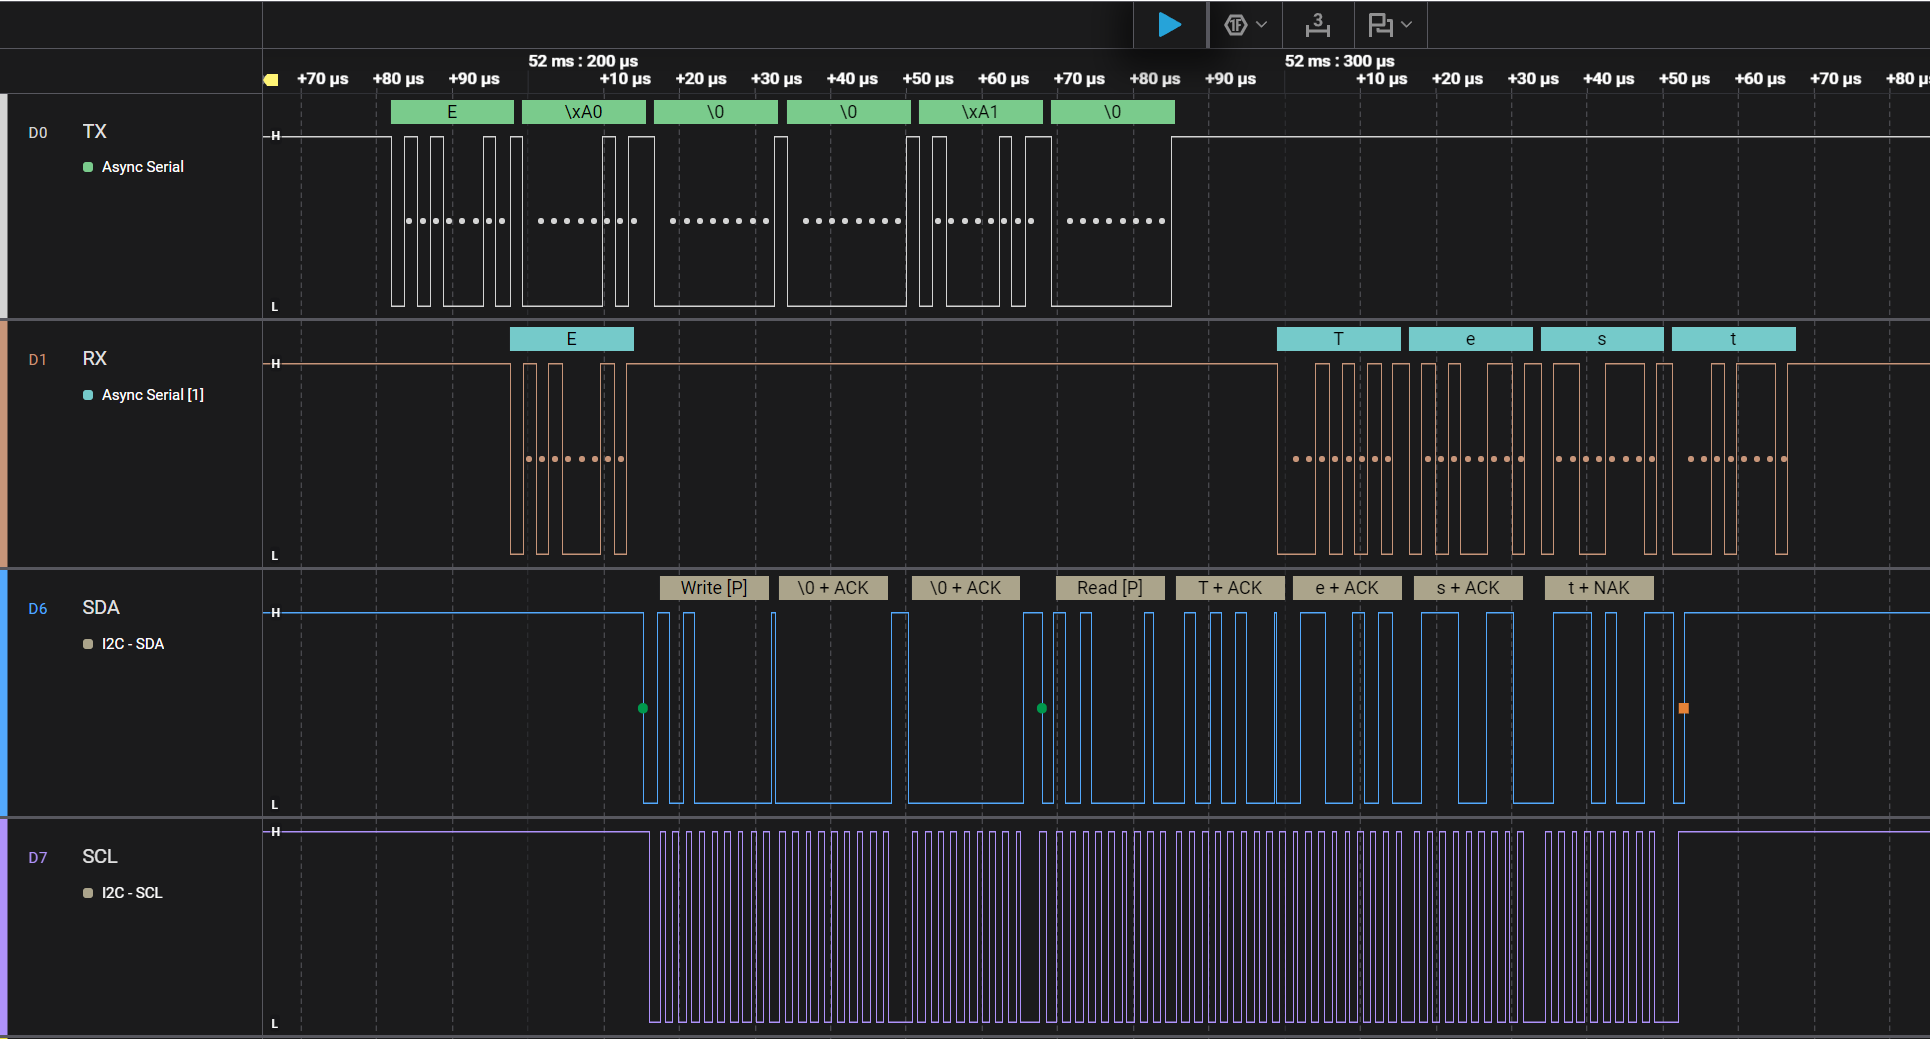
\includegraphics[trim=1mm 1mm 1mm 1mm,scale=0.3]{i2c small read.PNG}
	\caption{vizualizált analizátor rögzítés példa}
	\label{vizualizált analizátor rögzítés példa}
\end{figure}


\subsection{UART}%done
Az általam készített programozó sok kommunikációs protokollt használ, köztük az UART-ot. A számítógéppel való kommunikálás UART-on keresztül történik, a FTDI232 UART-USB átalakító segítségével.

Az UART (Universal Asynchronous Receiver Transmitter) egy kommunikációs protokoll, amely aszinkron, teljes duplex és soros. Az, hogy soros azt jelenti, hogy az adatátvitel bitenként történik, nem párhuzamos vonalokon. Az, hogy aszinkron azt jelenti, hogy nem létezik külön órajel vonal; az időzítést a küldő és a fogadó egymástól függetlenül szabályozza. És az, hogy teljes duplex azt jelenti, hogy két irányú adatátvitel valósul meg egyidejűleg.
Az adatokat "keretek” alakjában továbbítja, ahol egy tipikus adatkeret tartalmaz egy kezdő (start) bitet, adatbiteket, opcionális paritásbitet a hibakezeléshez, majd egy stop bitet. A start és stop bitek segítik a fogadó eszközt abban, hogy pontosan meghatározza az adatcsomagok kezdetét és végét, és ezáltal megbízható adatátvitelt biztosítanak.

A Baud ráta a kommunikációs rendszer azon paramétere, amely megadja, hogy másodpercenként hány szimbólum van a vonalon küldve, azaz hány darab jelváltás történik a vonalon. A beállított Baud ráta alapján van a fogadó vonal mintavételezésé, és a küldő vonalon a jel váltás időzítve.

Az UART egyszerűsége és hatékonysága miatt elterjedt megoldás a mikrovezérlők, számítógépek és egyéb beágyazott rendszerek közötti kommunikációban.

Használt forrás: \cite{tiuart}
%done
\begin{figure}[H]
	\centering
	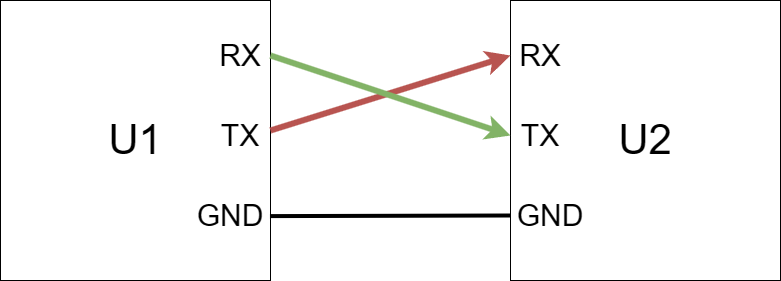
\includegraphics[trim=1mm 1mm 1mm 1mm,scale=0.8]{uartblock.png}
	\caption{UART blokkvázlat}
	\label{UARTblockk}
\end{figure}
A fenti blokkvázlaton egy UART elrendezés van rajzolva. A TX jelölés a "Transmit" (küldés) jelölésé, míg az RX a "Receive" (fogadás) jelölésé. Nem szükséges minden vonalat használni, lehet szimplex, fél-duplex vagy teljes duplex a kommunikáció. Szimplex lenne, ha az csak a U1 Tx és U2 RX lába között lenne kapcsolat, ebben az esetben az adatátvitel egyirányú lenne, tehát csak küldésre lenne lehetőség. Fél- vagy teljes duplex konfiguráció esetén az áramkört a mellékelt ábrának megfelelően kell elrendezni. Ha az U1 és U2 képes egyidejűleg adatot küldeni és fogadni, a kommunikáció teljes duplex-ként működik, ha nem akkor fél duplex. A programozón teljes duplex a kommunikáció.%done

\begin{figure}[H]
	\centering
	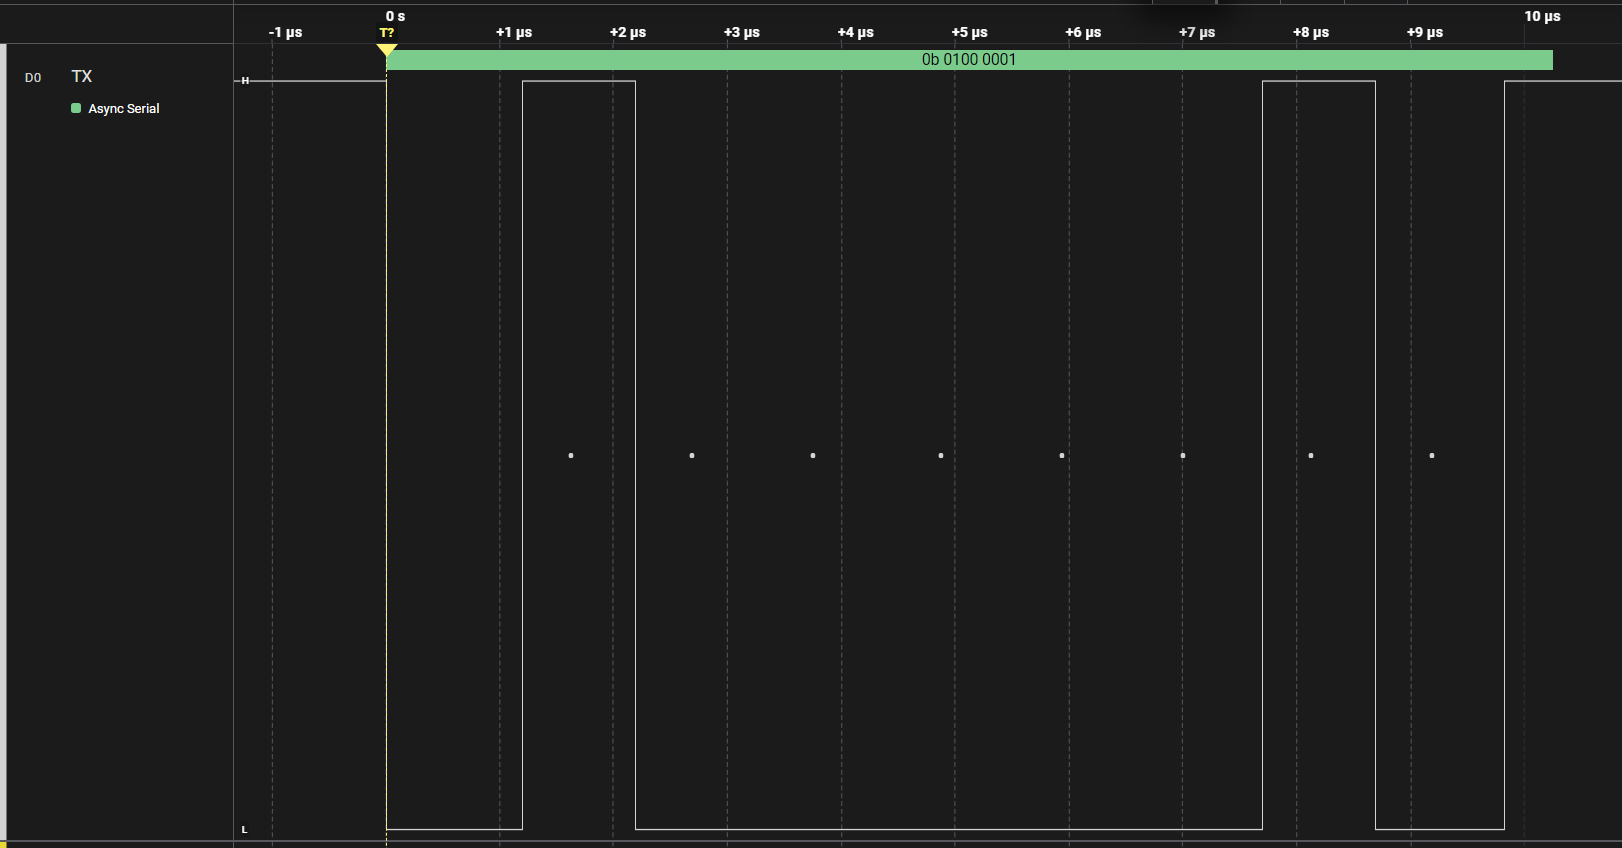
\includegraphics[trim=1mm 1mm 1mm 1mm,scale=0.35]{UARTfromAnalyzer.PNG}
	\caption{UART adatkeret}
	\label{UARTkep}
\end{figure}
A fenti képen egy adatkeret szerepel. Ezt az adatkeretet az FPGA küldte a programozónak. A Baud ráta ebben az esetben 921600 Baud, egy szimbólum ideje: 1/921600 Baud = 1.09 μs. Ez az analizátor program segítségével látható a képen.

Látható a start bit. A start bit után következik 8 adatbit, amik a programozó által küldött parancsot tartalmazzák. És végül a stop bit után a vonal visszatér a tétlen állapotba.%done

\subsection{SPI}
Az SPI (Serial Peripheral Interface) egy széles körben használt és rugalmas kommunikációs protokoll. Teljes duplex, és szinkron módon működik, az UART-tal ellentétben.%done
\begin{figure}[H]
	\centering
	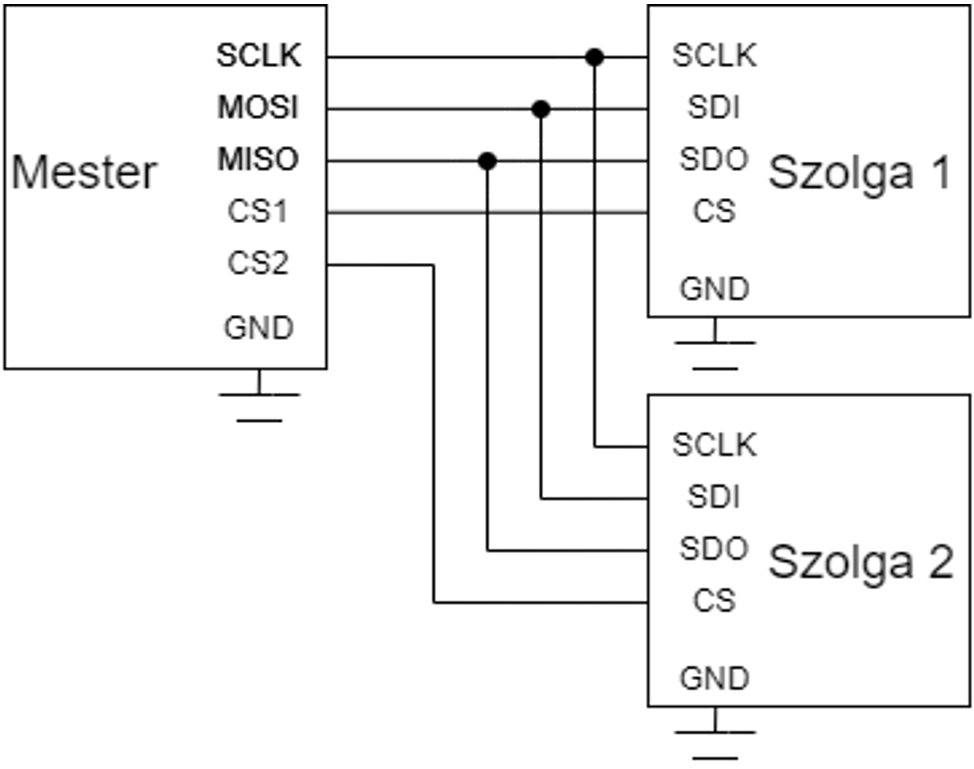
\includegraphics[trim=1mm 1mm 1mm 1mm,scale=0.4]{SPIblockk.PNG}
	\caption{SPI blokkvázlat}
	\label{SPI blokkvázlat}
\end{figure}
Az SPI protokoll előnye, hogy lehetővé teszi, hogy több IC megossza ugyanazokat a kommunikációs vonalakat, de egyszerre csak egy mester és egy szolga lehet aktív. Minden szolgához külön CS vonal szükséges, míg az egyéb vonalak (MISO, MOSI, SCLK) közösek lehetnek. A mester választja ki az adott szolgát az adott szolga chip select vonalán keresztül, és indítja a kommunikációt. A szolga kizárólag kiválasztott állapotban képes adatátvitelre. Ennek megfelelően egy szolgának négy, a mesternek három lábra, plusz egy további lábra per darab szolga, van szüksége.%done


Az SPI szinkron protokoll. Ezért kell az SCLK, vagyis az órajel vonal. Ez azt jelenti, hogy nincs előre beállított adatátviteli sebesség. A mester előállít egy órajelet a SCLK vonalon, a szolgák pedig az órajel éleit figyelve mintavételeznek és küldenek adatot. Így az adatátviteli sebesség az órajel frekvenciájától függ. Ezért az órajelnek nem kell a kommunikáció alatt ugyan azon a frekvencián maradni. Ezt ki is használom a programozómban. Az órajel ki van "nyújtva" és megállítva amikor a programozó várja a következő adatot a felhasználótól az UART vonalon.%done 


A MISO magyarul "mester be szolga ki”, a MOSI pedig "mester ki szolga be”. SPI-t használó IC-k lábai lehetnek jelölve SDI-ként (soros adat be) meg SDO-ként (soros adat ki). %done

Használt forrás: \cite{tispi}
\begin{figure}[H]
	\centering
	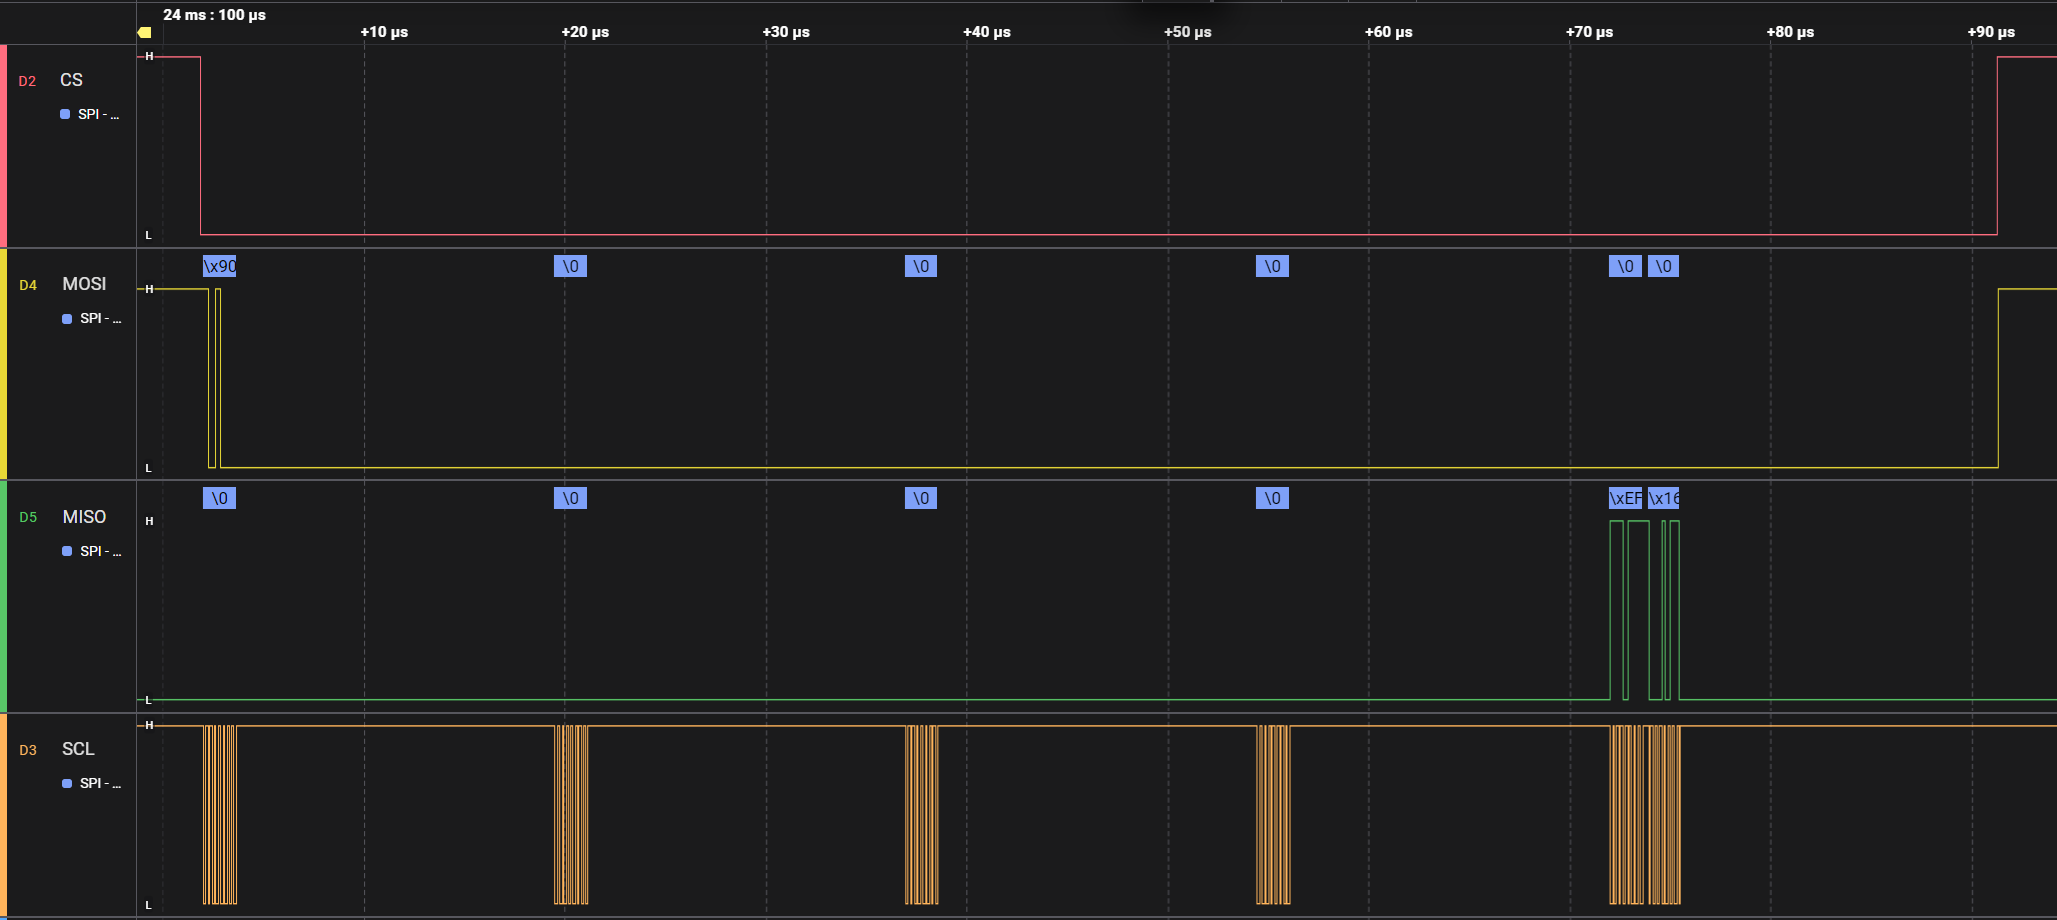
\includegraphics[trim=1mm 1mm 1mm 1mm,scale=0.28]{SPIreadID.png}
	\caption{SPI-al kiolvasott gyártó azonosító és típusszám}
	\label{SPI-al kiolvasott gyártó azonosító és típusszám}
\end{figure}
Itt látható egy példa egy SPI kommunikációra. Ez a kommunikáció a programozó és egy W25Q64JV Flash memória között történt. A termék gyártó azonosítóját (xEF) és típusszámát (x16) olvasom ki \cite{FLASH}.
A CS vonal kiválasztja a Flash modult, majd kezdődik a kommunikáció. Ahhoz, hogy kiolvassuk az azonosítókat a modulnak a x90 instrukciót kell küldeni, majd 3 bájtin x00 címet \cite{FLASH}.
Látszik az órajel nyújtás is, ami azért kell, mert a programozó várja a következő írandó bájtot az UART vonalon a PC-től. Többet írok erről a következő fejezetekbe.
Amint az olvasás kész, és a programozó elküldte az adatot a PC-nek UART-on, a CS vonal visszalép magas szintbe és véget ér a kommunikáció. %done

\subsection{I2C}

Az I2C egy soros, szinkron, kétvezetékes kommunikációs protokoll, Az I2C célja, hogy egyszerű és hatékony adatcserét tegyen lehetővé rövid távolságon belül egy mester, más néven vezérlő, és több szolga, azaz célpont, eszköz között. Az egyszerűsége miatt széles körben alkalmazott.

\begin{figure}[H]
	\centering
	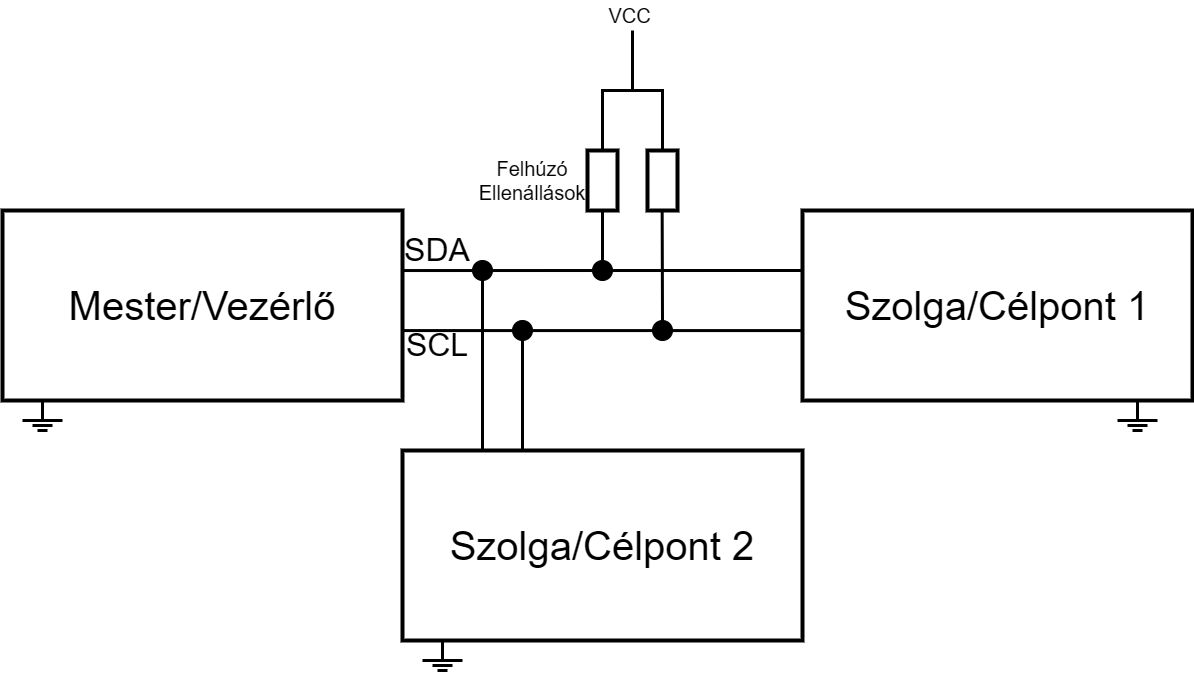
\includegraphics[trim=1mm 1mm 1mm 1mm,scale=0.335]{i2cblokk.png}
	\caption{I2C elrendezés példa blokkvázlat}
	\label{I2C elrendezés példa blokkvázlat}
\end{figure}

A fenti képen egy általam rajzolt példa elrendezés látható. A protokoll két vonalat használ: az SDA, azaz soros adat, és az SCL, magyarul soros órajel, vezetéket. A szabvány szerint a vonalak nyitott kollektoros kialakításúak, ezért minden eszköz csak lehúzni tudja őket. Felhúzó ellenállások biztosítják az alapértelmezett magas szintet. Az I2C szinkron protokoll, vagyis az adatátvitel órajel vezérelt, az SCL vonalat mindig a mester generálja, így a sebességet is ő szabja meg. 

A protokoll a címalapú kommunikáción alapul: minden szolga eszköz rendelkezik egy egyedi címmel, és a mester ennek megfelelően kezdeményezi az adatcserét. Ezért nem kell minden szolgának egy külön CS vonal, mint az SPI-nál.

A programozóban az I2C protokollt úgy implementáltam, hogy az órajel nyújtás is lehetséges legyen. Ez lehetővé teszi, hogy a programozó várjon a felhasználói parancsra UART-on keresztül, mielőtt az I2C kommunikáció folytatódna.

Használt forrás: \cite{ti3c}
\begin{figure}[H]
	\centering
	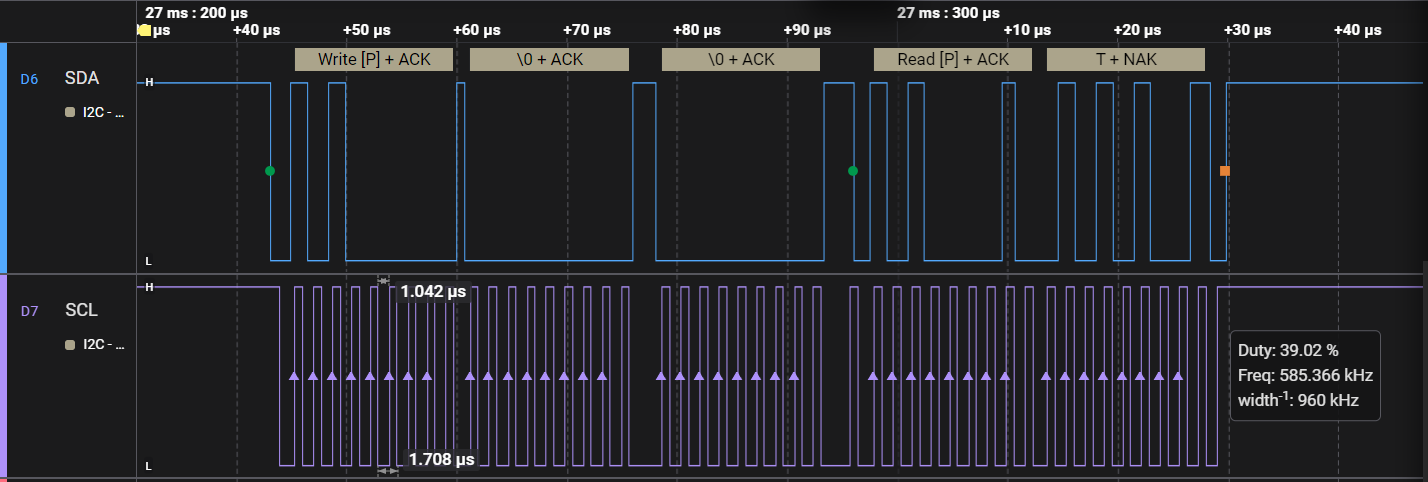
\includegraphics[trim=1mm 1mm 1mm 1mm,scale=0.41]{i2creadmini.PNG}
	\caption{I2C 1 bájtos olvasás a programozóval}
	\label{I2C 1 bájtos olvasás a programozóval}
\end{figure}
A fenti képen egy egybájtos I2C olvasási művelet látható, amely az EEPROM memóriamodul és a programozó közötti adatcserét rögzíti. 

Az adatátvitel egy START jellel kezdődik: a programozó előszőr a SDA vonalat logikai ’0’-ra húzza majd a SCL vonalat is.  Utána folytatódik a kommunikáció írási művelettel: a programozó az EEPROM címét (7 bites cím + írási bit) továbbítja. A memória eszköz ACK jellel válaszol. Ezután a programozó elküldi a memóriacímet (x0000), amely a kívánt olvasási cím regisztere. Ezt is ACK követi. Ez egy ”dummy write” \cite{EEPROM}, ami azért szükséges, hogy az EEPROM betöltse az adott regiszter értékeit, hogy később ki tudja őket küldeni.

A címzés után a programozó ismételt START jelet küld, egy úgynevezett "repeated START" \cite{EEPROM} jelet. Majd újra elküldi az EEPROM címét, ezúttal olvasási műveletet (read bit = 1) kérve. A szolga ACK jelzéssel visszaigazolja a fogadást, majd elküldi a kívánt adatbájtot. A programozó egy NAK jellel zárja az adatátvitelt, jelezve, hogy nem kíván további bájtokat olvasni, majd STOP jellel befejezi a kommunikációt: a SCL Vonalat logikai magasba engedi, majd a SDA vonalat is. 

A SCL vonalon a mért frekvencia ~585 kHz, ami a programozó beállított belső órajeléből számított értéknek felel meg. Az aktív ciklusidő 39.02\%, ez az órajelnyújtás, illetve a logikai műveletek időzítése miatt jelentkezik. A programozóban a I2C sebessége közelebb van az UART sebességéhez, mint az SPI sebessége, ezért nem olyan látványos az órajelnyújtás, mint az SPI rögzítésen látszódott. 

\chapter{Tervezés}
\section{A terv bemutatása}

\begin{figure}[H]
	\centering
	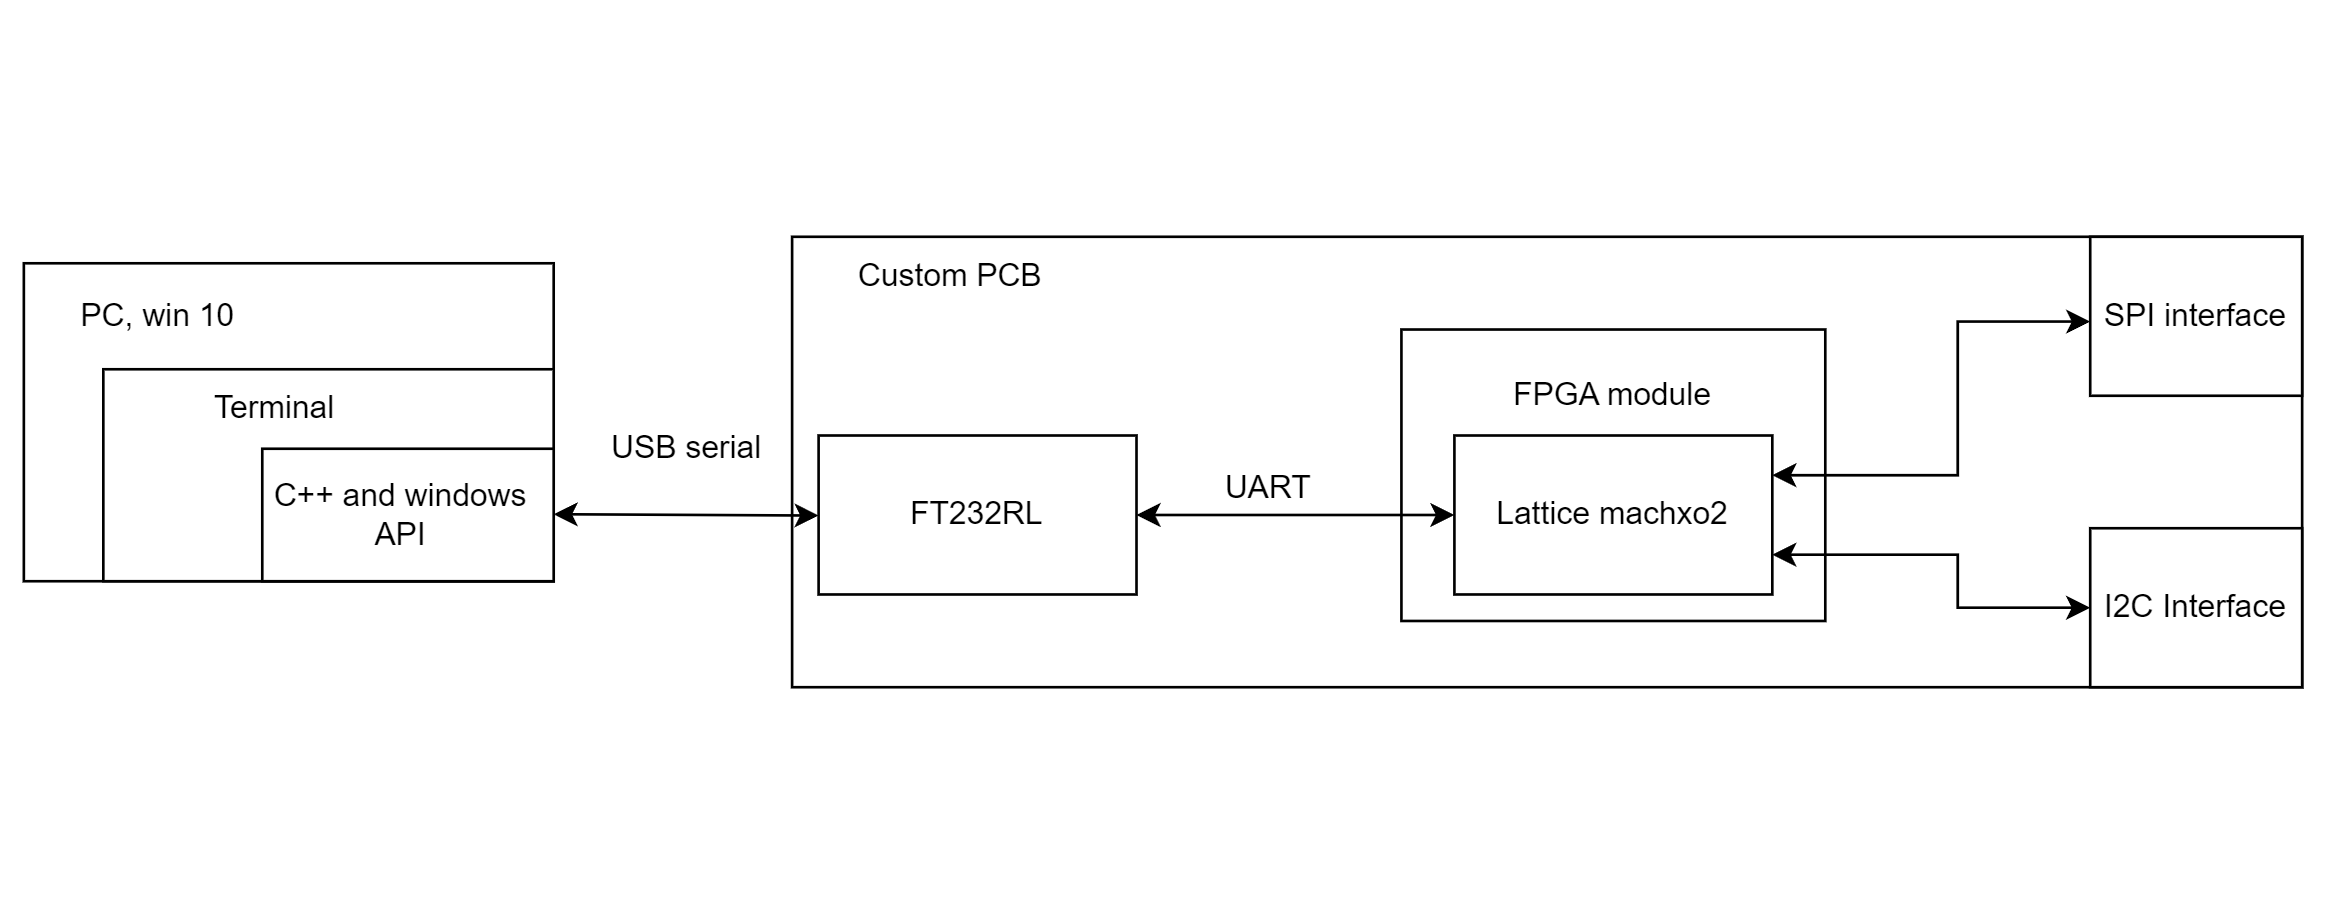
\includegraphics[trim=1mm 1mm 1mm 1mm,scale=0.245]{terv1.png}
	\caption{Projekt terv blokkvázlata}
	\label{Projekt terv}
\end{figure}
Ez a blokk diagramm volt a projekt kiinduló terve. A felhasználó a C++ -ban írt program futtatásával tud kommunikálni a programozóval terminálon keresztül. A küldödd USB kommunikációt a FT232RL váltja át UART csomagokká az FPGA modul számára. Az FPGA modulon megvalósított VHDL-ben megírt logikai áramkör, pedig a kapott parancsok alapján küld SPI és I2C parancsokat a programozandó EEPROM chipnek. Az EEPROM chip esetleges válaszait, pedig visszakonvertálja UART csomagokká az FT232RL-nek, amely visszaküldi a PC-nek.
\chapter{Megvalósítás}

\section{Kapcsolási rajz tervezése}

\begin{figure}[H]
	\centering
	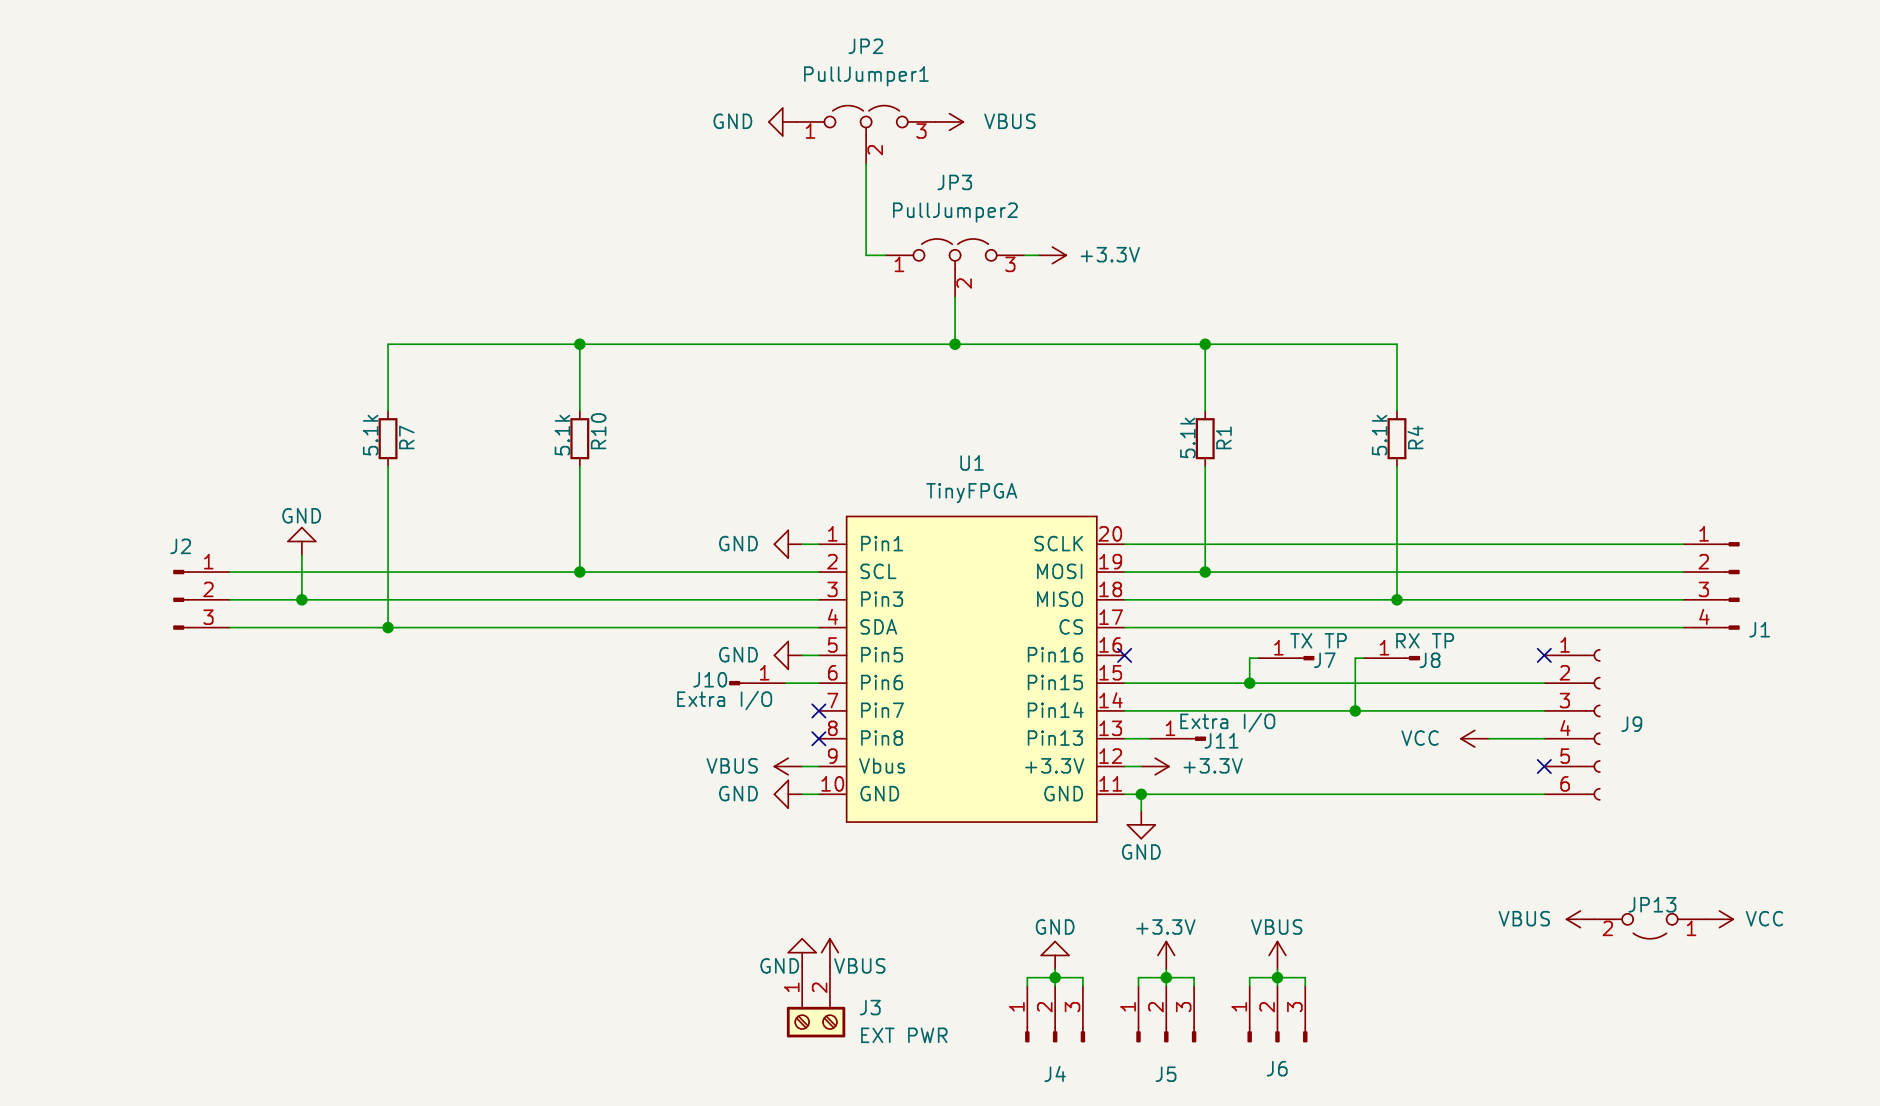
\includegraphics[trim=1mm 1mm 1mm 1mm,scale=0.30]{kapcsolasi rajz.PNG}
	\caption{A programozó kapcsolási rajza}
	\label{teljes kapcsolási rajz}
\end{figure}
A kapcsolási rajz viszonylag egyszerű, nincs sok alkatrész. A felhúzó ellenállásokat kivéve csak csatlakozók, és jumper-ek vannak a nyákon. Mégis sok időt fordítani a tervezésre.

A célom az volt, hogy ez egy általánosan használható EEPROM programozó legyen, ehhez rugalmasnak kellet megterveznem a nyákot.  A jumper-ek segítségével az ellenállások 3,3V vagy 5V felhúzó ellenállások, vagy akár lehúzó ellenállások ként is tudnak funkcionálni. Így sok féle memória modult tud támogatni az áramkör. Ha a JP2 jumper 1-es és 2-es pin-je van közösítve, akkor GND van kiválasztva. Ha a JP2 jumper 2-es és 3-es pin-je van közösítve, akkor 5V van kiválasztva. Ha a JP3 jumper 2-es és 3-es pin-je van közösítve, akkor 3,3V van kiválasztva.
\begin{figure}[H]
	\centering
	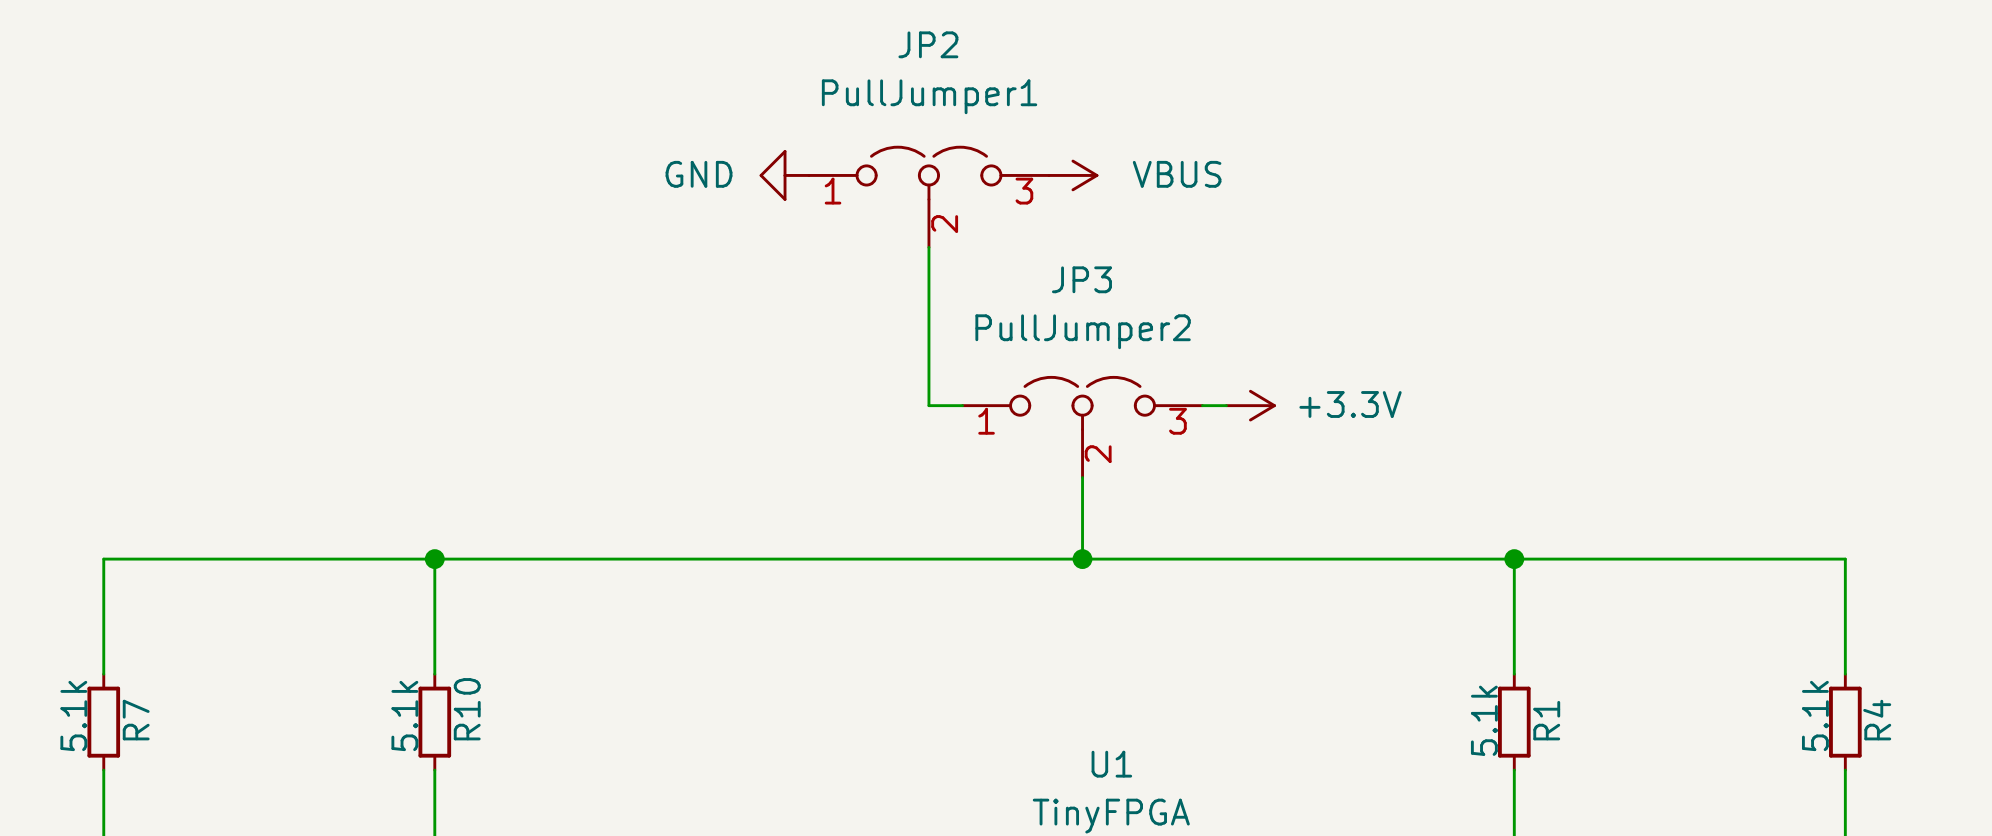
\includegraphics[trim=1mm 1mm 1mm 1mm,scale=0.29]{jumperek.PNG}
	\caption{Ellenállás jumper-ek}
	\label{Ellenállás jumper-ek}
\end{figure}
\begin{figure}[H]
	\centering
	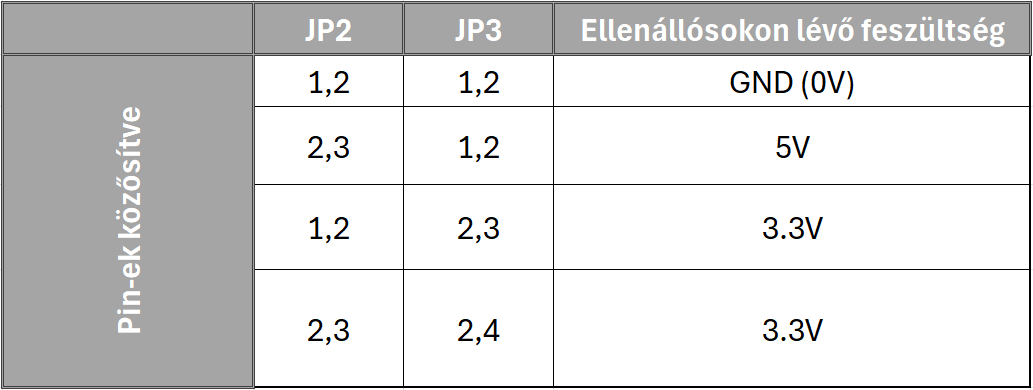
\includegraphics[trim=1mm 1mm 1mm 1mm,scale=0.45]{jumpertable.PNG}
	\caption{Ellenállások feszültségének összefüggése}
	\label{Ellenállások feszültségének összefüggése}
\end{figure}
Az áramkörnek 4 lehetséges tápja van
\begin{itemize}
	\item A TinyFPGA 5V VBUS pin-je. A pin közvetlen össze van kötve a modul mikró USB 5V tápjával. Tehát amikor a TinyFPGA modul csatlakoztatva van a mikró USB-n keresztül, a VBUS pin kimenetként szolgálhat. A TinyFPGA modul a betápját is a VBUS látja el. Szóval, ha a TinyFPGA nincs csatlakoztatva az USB-hez, akkor a VBUS pin bemenetként is működhet.
	\item A TinyFPGA 3V3 pin-je. Ezt a kimenetet a TinyFPGA modul LDO IC-je generálja a VBUS 5V feszültégéből.
	\item Az FTDI232 VCC kimenete. Ami állítható 3V3 és 5V között a FTDI232 modulon egy jumper-el.
	\item Az EXT PWR csatlakoztató. Amit a biztonság kedvéért raktam hozzá az áramkörhöz, ha szükség lenne a jövőben egy külső tápra.
\end{itemize}
A jumper-ek úgy vannak megtervezve, hogy bármelyik 5V-os bemenet szolgálhasson tápként a nyáknak, meg a hozzá csatolt memória moduloknak. De a legtöbbet használt konfiguráció, az a FTDI232 VCC kimenetét használja az 5V módban. Ilyenkor persze a JP13 jumper két pin-je közösítve kell hogy legyen, hogy a TINY FPGA megkapja a 5V táp feszültséget.
\begin{figure}[H]
	\centering
	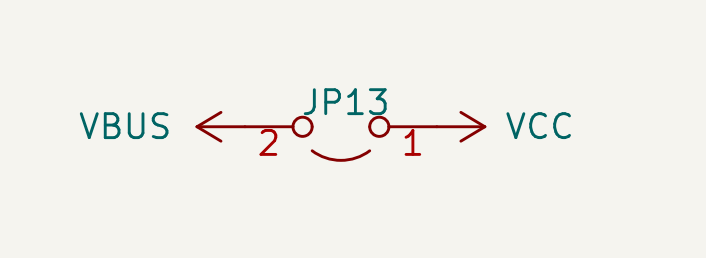
\includegraphics[trim=1mm 1mm 1mm 1mm,scale=0.45]{JP13.PNG}
	\caption{VCC és VBUS közösítő jumper}
	\label{VCC és VBUS közösítő jumper}
\end{figure}
A nyákon ki van vezetve három, három pin-en a GND, 3V3, és a VBUS. Ezek a csatlakozók tápként szolgálnak a csatlakoztatott memória moduloknak, illetve merési pontoknak is alkalmasak.
\begin{figure}[H]
	\centering
	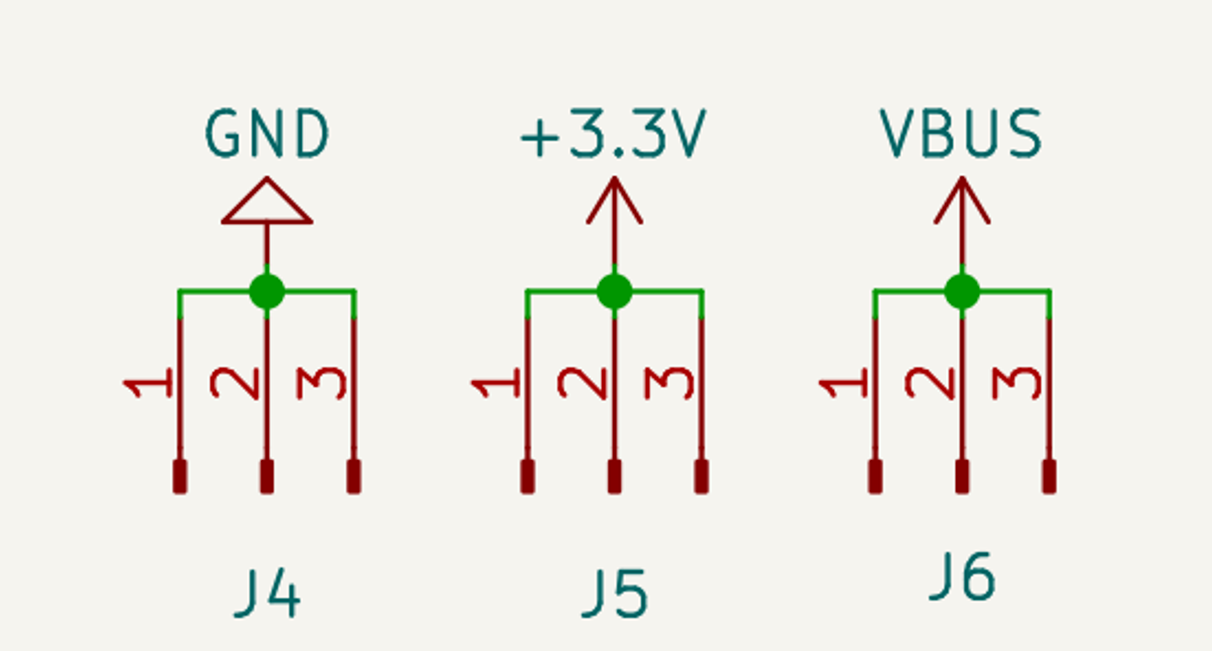
\includegraphics[trim=1mm 1mm 1mm 1mm,scale=0.45]{gnd5v3v3.PNG}
	\caption{Fontos feszültségek és a GND kivezetése}
	\label{Fontos feszültségek és a GND kivezetése}
\end{figure}
\subsection{Nyák tervezése}
\begin{figure}[H]
	\centering
	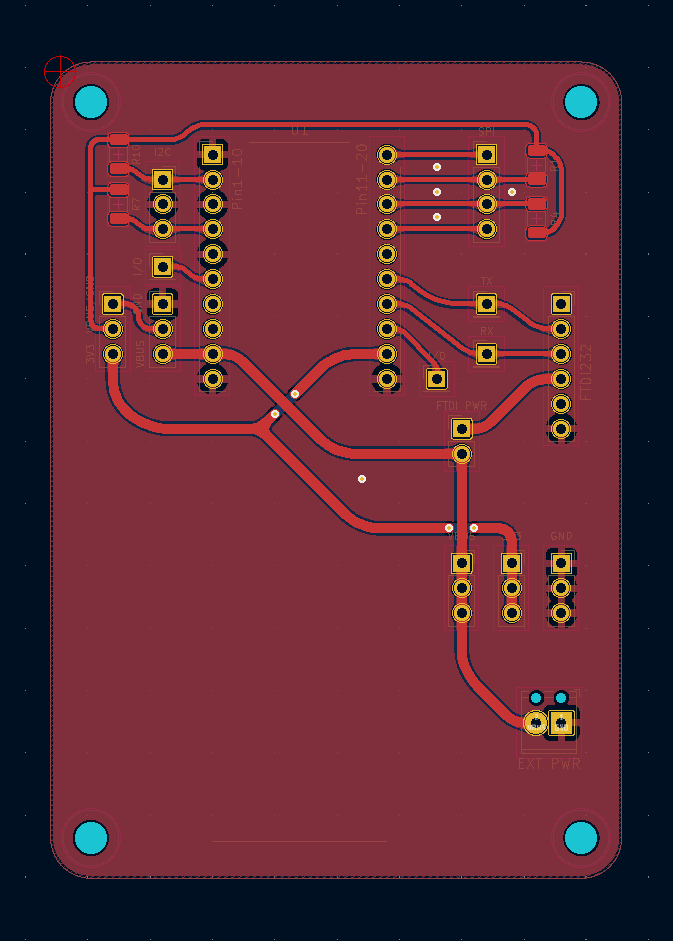
\includegraphics[trim=1mm 1mm 1mm 1mm,scale=0.4]{nyak.PNG}
	\caption{A programozó Nyák-ja}
	\label{A programozó Nyák-ja}
\end{figure}
A fenti ábra a végleges nyák terv, aminek gyártását megrendeltem. Egy két rétegű egyszerű nyák. Egy ilyen egyszerűbb nyák tervezése közben is fontos betartani az alapszabályokat.

Tervezés előtt kell beállítani a gyártási limiteket. Ha tudjuk, hogy melyik céget akarjuk megrendelni a nyákot, akkor a weboldalukon megtalálhatjuk ezeket az értékeket. A limiteket a "Board Setup" funkcióval lehet megadni. Ha jól vannak megadva az értékek, akkor a KiCad nem enged olyan nyákot tervezni, amit nem tud a nyák gyártó cég legyártani. Az én esetemben:
\begin{figure}[H]
	\centering
	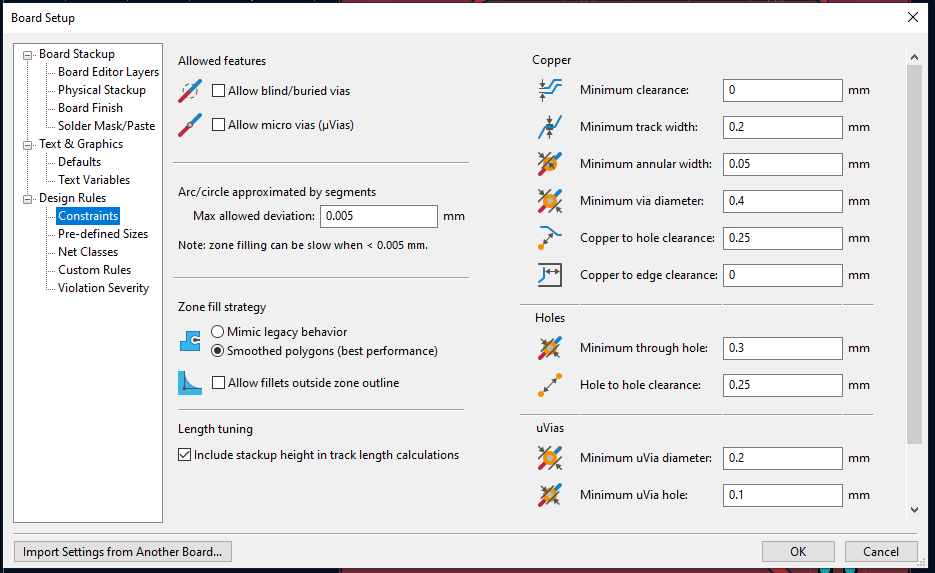
\includegraphics[trim=1mm 1mm 1mm 1mm,scale=0.5]{bosrd limits.PNG}
	\caption{KiCad limit beállítások}
	\label{KiCad limit beállítások}
\end{figure}
\subsubsection{A nyák alsó rétege}
A hátsó réteg itt egyszerű. Az egész egy GND réteg, minél kevesebb megszakítással, hogy minimalizálva legyenek az áramok visszaútjai, és ezáltal az arámhurkok területei is.
\begin{figure}[H]
	\centering
	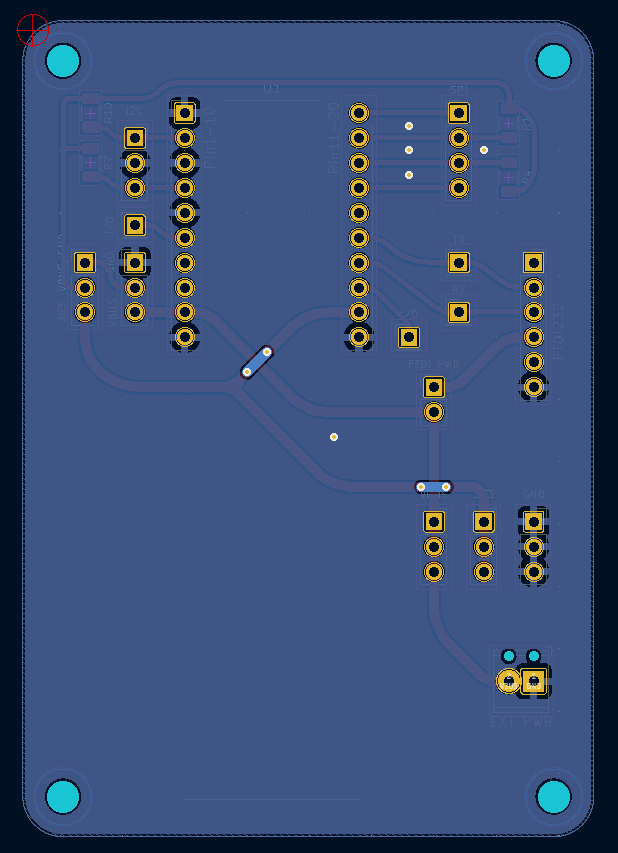
\includegraphics[trim=1mm 1mm 1mm 1mm,scale=0.4]{also reteg.PNG}
	\caption{A nyák alsó rétege}
	\label{A nyák alsó rétege}
\end{figure}
\subsubsection{Az SPI csatlakozó}
\begin{figure}[H]
	\centering
	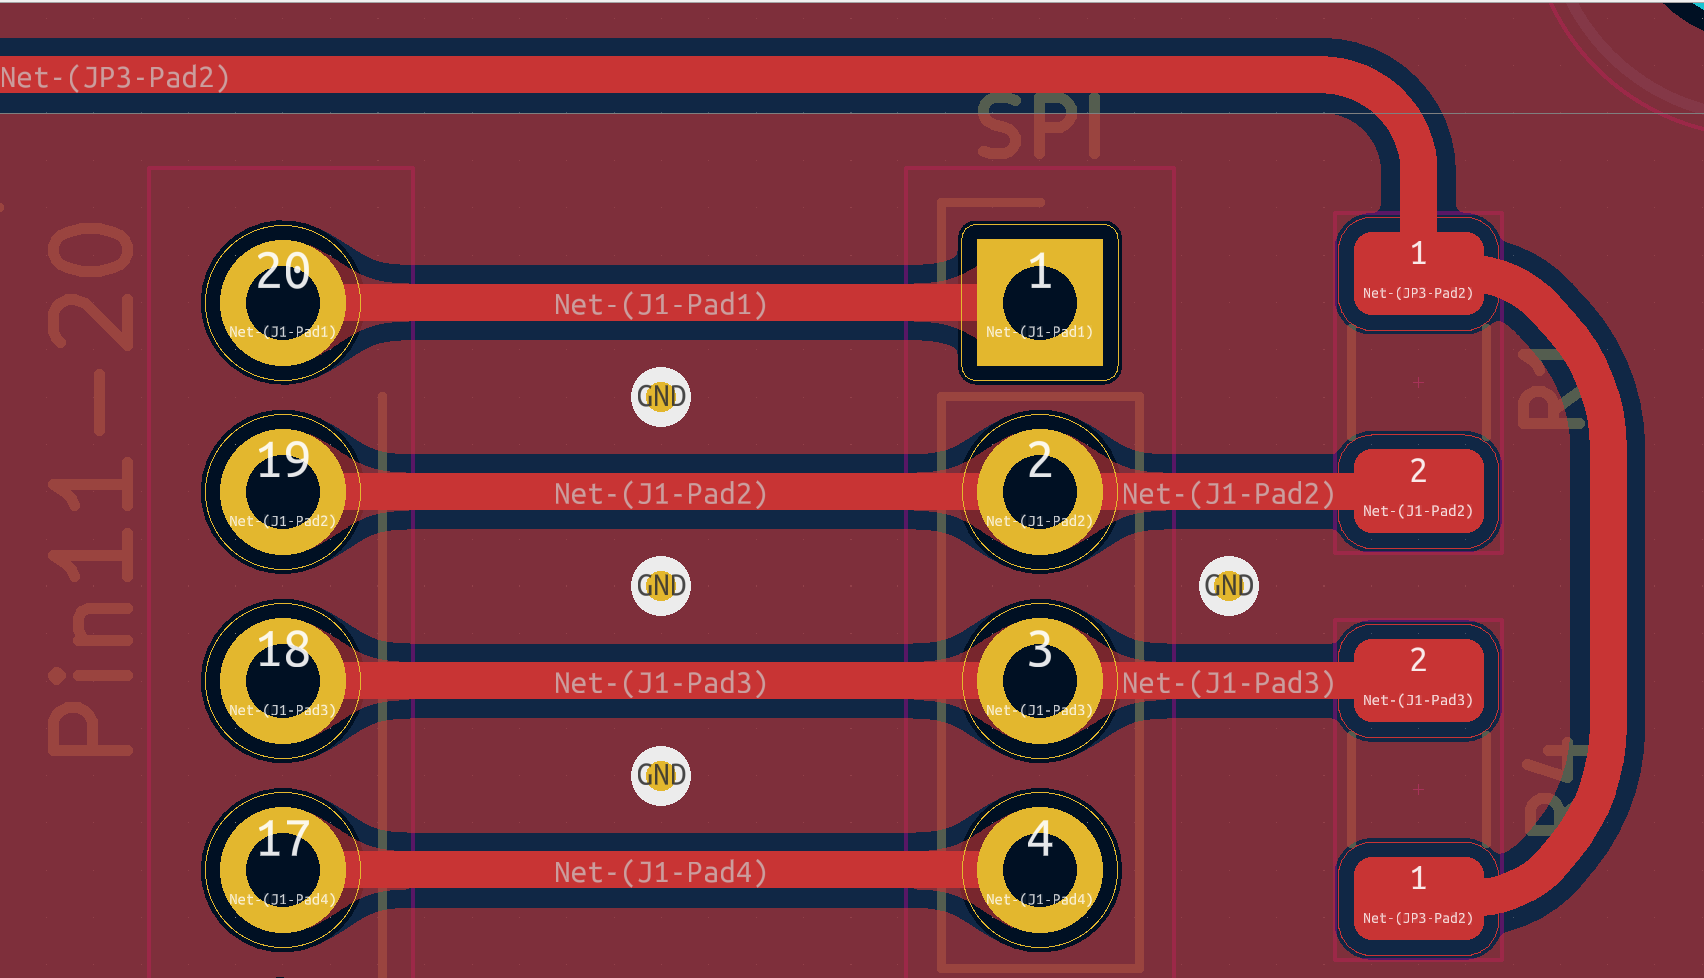
\includegraphics[trim=1mm 1mm 1mm 1mm,scale=0.3]{spi kimenet.PNG}
	\caption{SPI kimenet}
	\label{SPI kimenet}
\end{figure}
Kissé túl van tervezve az SPI csatlakozó, hiszen nem óriási frekvenciákon használom. De a túltervezés ebben az esetben nem árt. A chip select, MISO, MOSI, és CLK vonalak mind ugyan olyan hosszúak. Ezt "length matching”-nek hívjuk. Akkor fontos, ha akkora az adatátviteli alap frekvencia, hogy két vonal hossz különbségéből származó kettő közötti fázistolás, gondot okoz a mintavételezésnél. A vonalak egymástól GND-vel le vannak árnyékolva, ez segíti, hogy a vonalak elektromágneses zajai kevésbé befolyásolják egymást.
\subsubsection{Az I2C csatlakozó}
\begin{figure}[H]
	\centering
	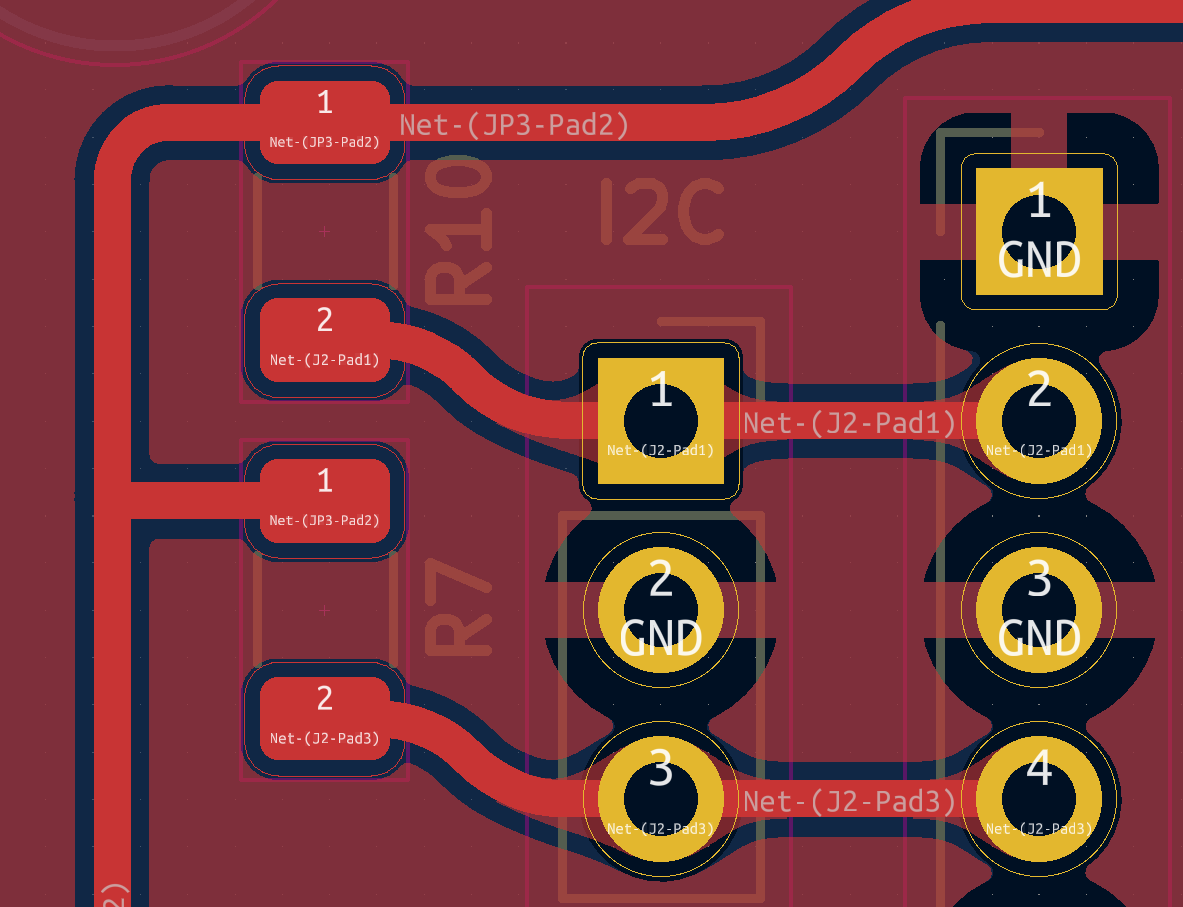
\includegraphics[trim=1mm 1mm 1mm 1mm,scale=0.38]{i2ckimenet.PNG}
	\caption{I2C kimenet}
	\label{I2C kimenet}
\end{figure}
Itt is inkább túlterveztem a kimenetet, mint alul. A SCL és SDA vonal "length match”-elve van. Illetve az árnyékolás még a csatlakozókra is kiterjed. Így egészen a FPGA lábaihoz leht vinni az árnyékolást, ha a SCL és SDA-hez tartozó lábak közötti pin-t logikai ’0’-ra állítom.
\subsubsection{Bővítmények}
Két bővítményt használtam. Az egyik a "rounded tracks bővítmény". Ami igazából csak esztétikai változásokat csinál a nyákon.
A bővítményt nagyon egyszerű használni. A következő kép a UI-ja.
\begin{figure}[H]
	\centering
	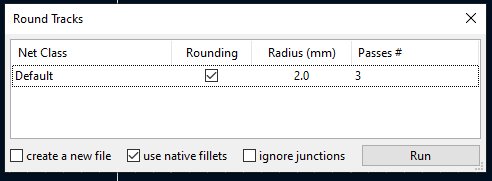
\includegraphics[trim=1mm 1mm 1mm 1mm,scale=0.75]{rounded ui.PNG}
	\caption{A rounded tracks bővítmény UI-ja}
	\label{A rounded tracks bővítmény UI-ja}
\end{figure}
A UI egyszerű. Netlistaként ki lehet választani, hogy kerekítse a bővítmény a netlistához tartozó trace-eket vagy nem. Ki lehet választani célzott rádiuszt, illetve, hogy hányszor fusson a program. A "run" gombbal kell elindítani.

Ezek pedig arról képek, hogy hogyan néz ki egy trace a bővítmény használata előtt és utána.

\begin{figure}[H]
	\centering
	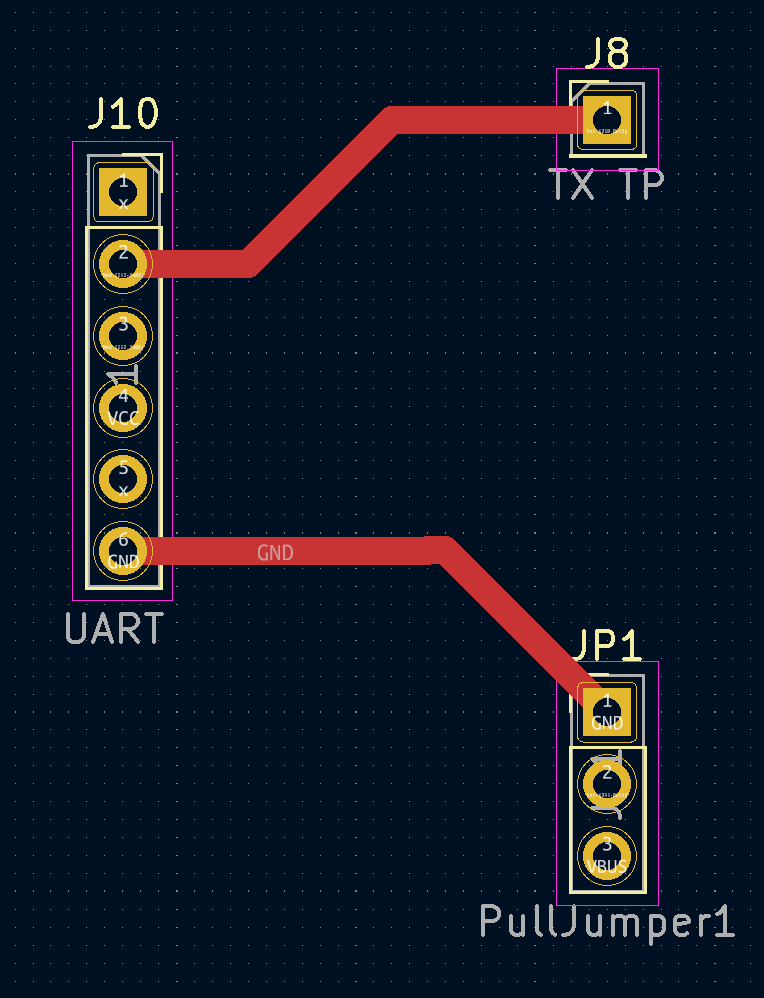
\includegraphics[trim=1mm 1mm 1mm 1mm,scale=0.35]{beforrounded.PNG}
	\caption{Egy trace a bővítmény használata előtt}
	\label{Egy trace a bővítmény használata előtt}
\end{figure}
\begin{figure}[H]
	\centering
	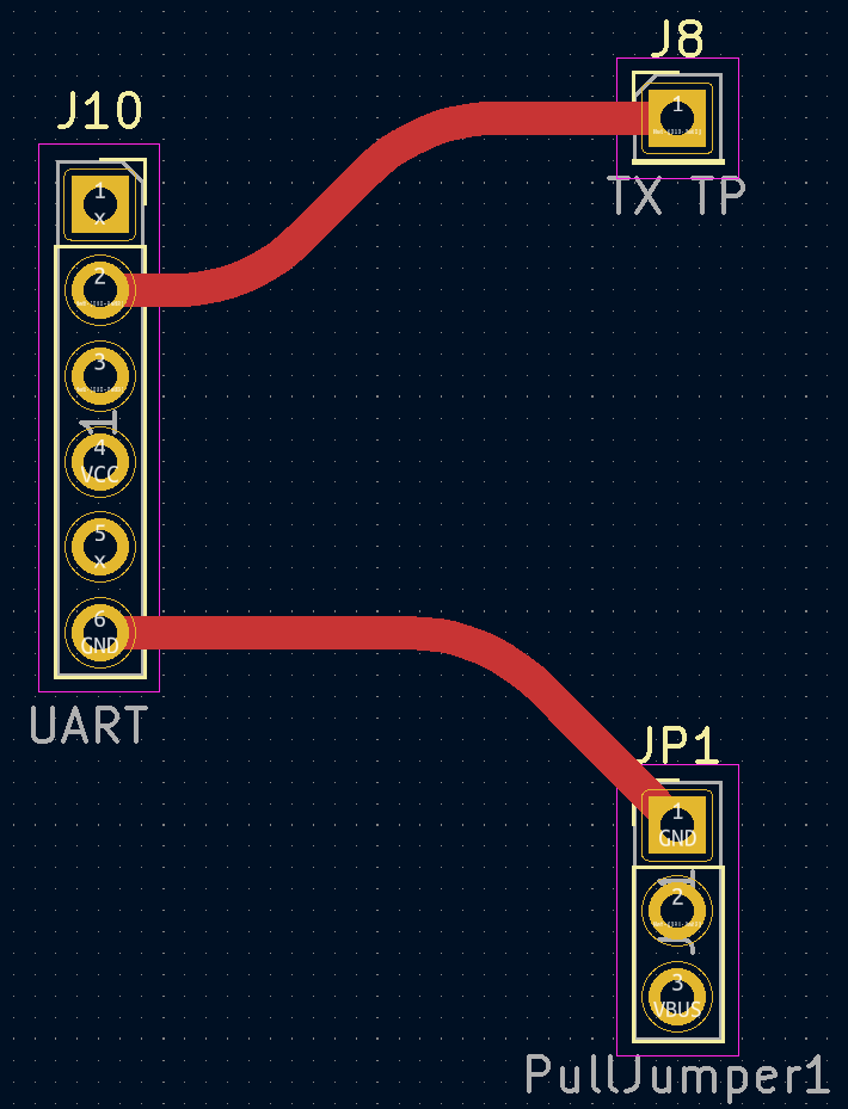
\includegraphics[trim=1mm 1mm 1mm 1mm,scale=0.35]{afterrounded.PNG}
	\caption{Egy trace a bővítmény használata után}
	\label{Egy trace a bővítmény használata után}
\end{figure}
Fontos, hogy a bővítmény használata előtt nézzük át a tarce-einket. A bővítmény nem működik jól, ha túl sok elemre bontott, csúnyán tervezett trace-et akarunk kerekíteni.
\begin{figure}[H]
	\centering
	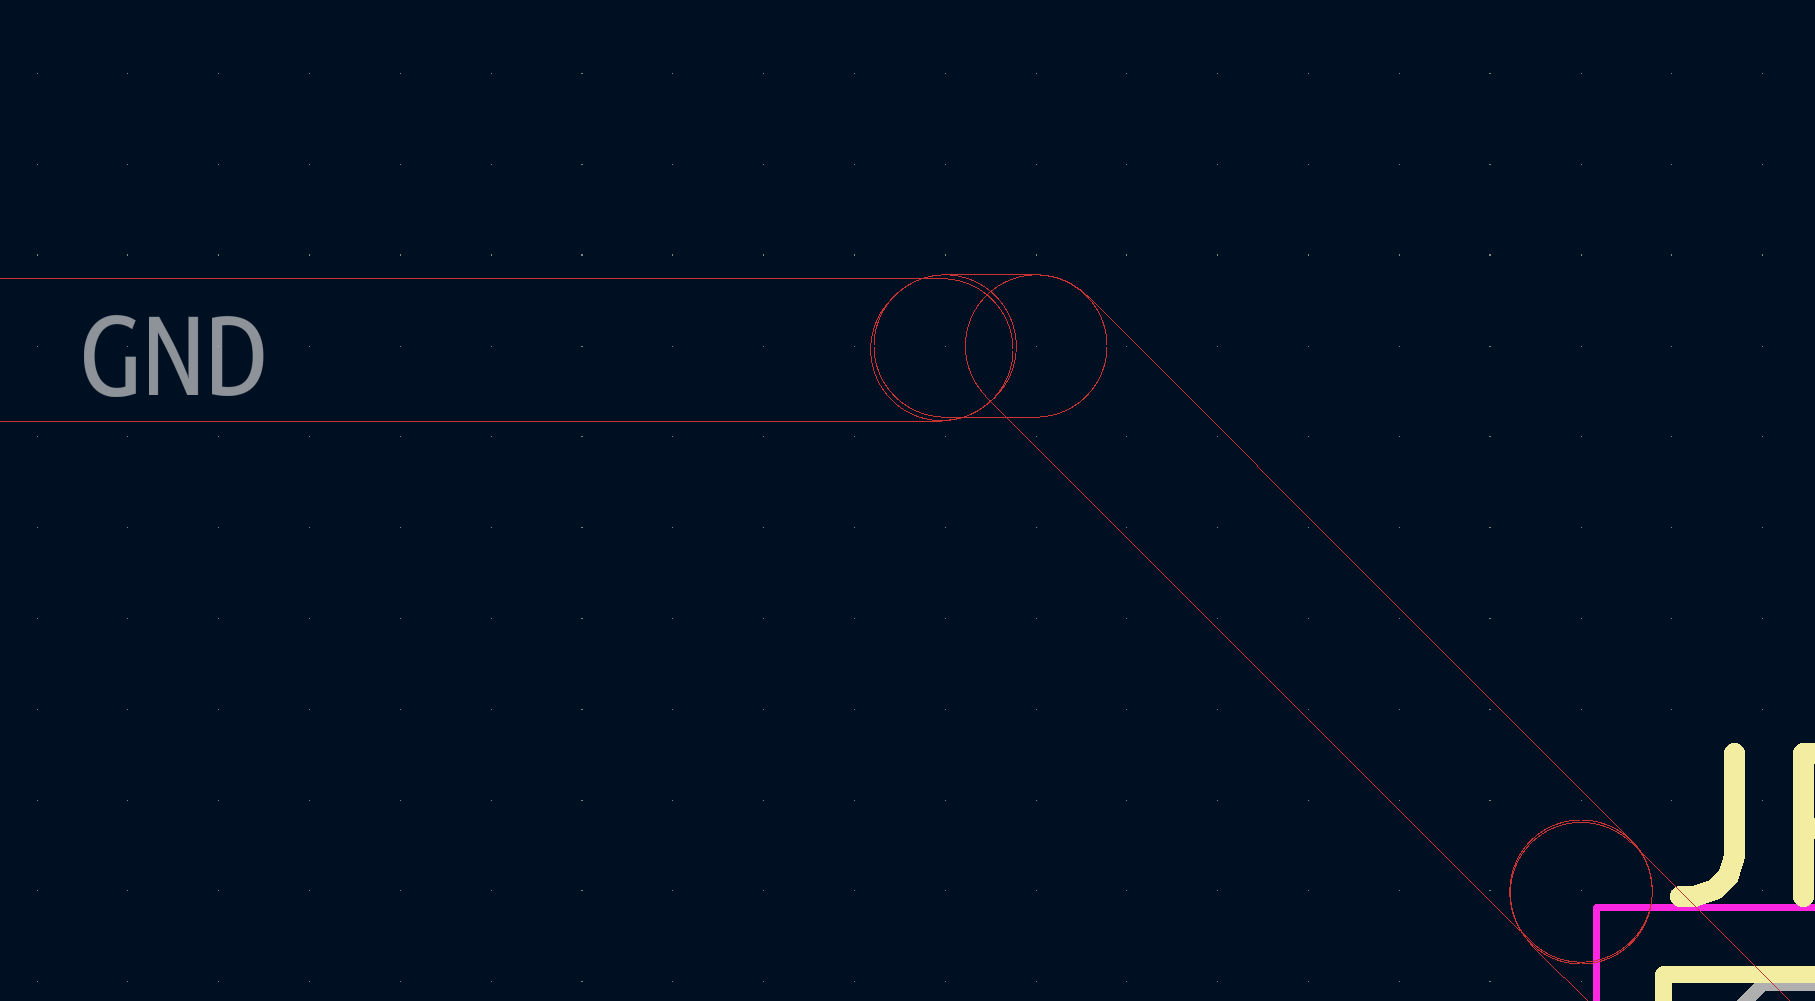
\includegraphics[trim=1mm 1mm 1mm 1mm,scale=0.25]{rosszpelda.PNG}
	\caption{Példa egy csúnyán tervezett trace-re}
	\label{Példa egy csúnyán tervezett trace-re}
\end{figure}
A másik bővítmény pedig, a "Teardrop vias" bővítmény. Ez a bővítmény, ami részben esztétikailag is szépíti a nyák tervet, de fontos, hogy az éles sarkokat is minimalizálja. Hiszen az éles sarkok savcsapdákat okozhatnak, ahol a maratáshoz használt sav egy része megmarad, és az éles sarkoknál tovább korrodálja a rezet mint kellene. A következő kép a UI-ja.
\begin{figure}[H]
	\centering
	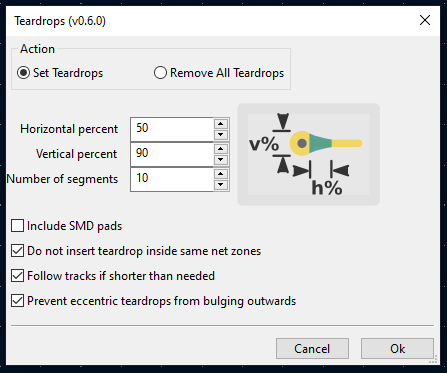
\includegraphics[trim=1mm 1mm 1mm 1mm,scale=0.75]{rounded vias ui.PNG}
	\caption{Teardrop vias UI} 
	\label{Teardrop vias UI}
\end{figure}
Ezek pedig arrol képek, hogy hogyan néz ki egy via a bővítmény használata előtt és utána.
\begin{figure}[H]
	\centering
	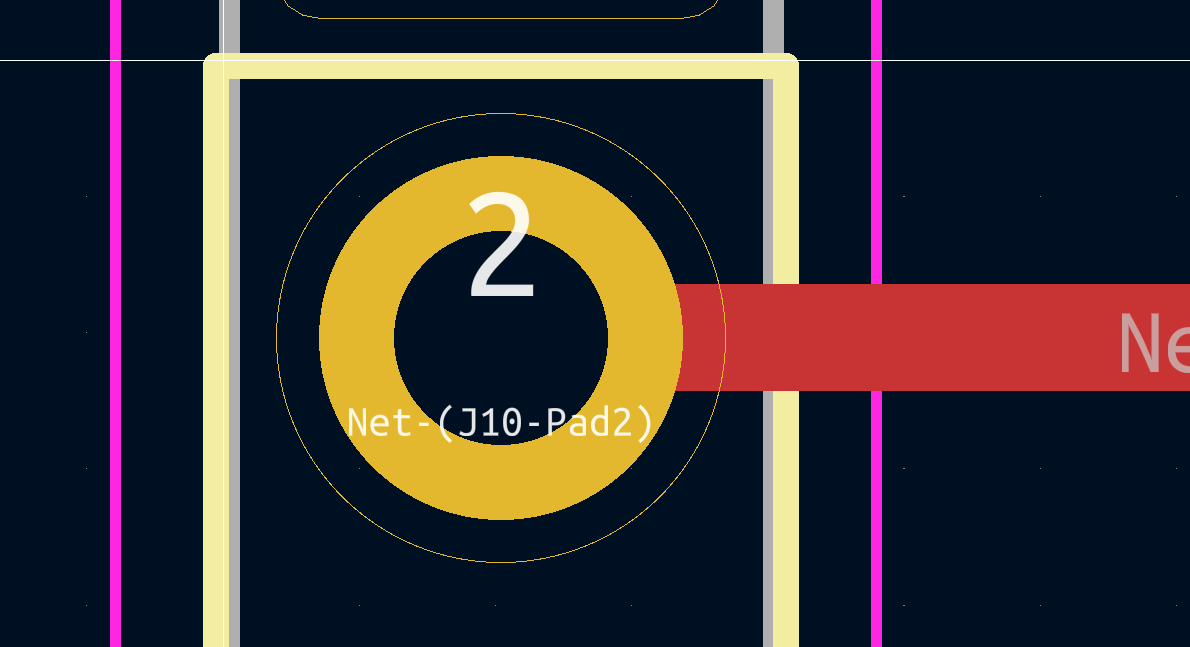
\includegraphics[trim=1mm 1mm 1mm 1mm,scale=0.4]{viabefore.PNG}
	\caption{Teardrop bővítmény használata előtt}
	\label{Teardrop bővítmény használata előtt} 
\end{figure}
\begin{figure}[H]
	\centering
	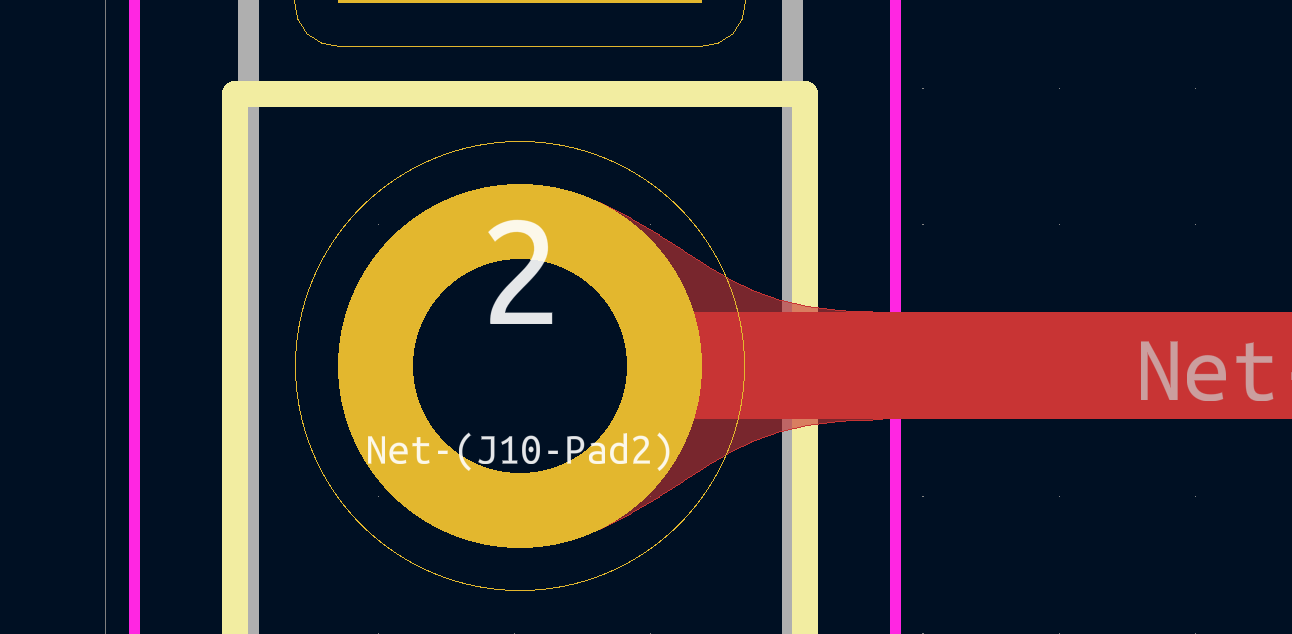
\includegraphics[trim=1mm 1mm 1mm 1mm,scale=0.4]{viaafter.PNG}
	\caption{Teardrop bővítmény használata után}
	\label{Teardrop bővítmény használata után} 
\end{figure}
\section{Az elkészült nyák}
\begin{figure}[H]
	\centering
	\includegraphics[trim=1mm 1mm 1mm 1mm,scale=0.1]{PCB.png}
	\caption{A kész nyák}
	\label{A kész nyák} 
\end{figure}
\begin{figure}[H]
	\centering
	\includegraphics[trim=1mm 1mm 1mm 1mm,scale=0.125]{PCBassembled.png}
	\caption{A kész nyák összeszerelve és forrasztva}
	\label{A kész nyák összeszerelve és forrasztva} 
\end{figure}

\section{A programozó alentitásai}
A következőkben bemutatom az alentitásokat, amiket használtam a programozóban. Ezeket én terveztem és írtam meg, kivéve az Int\_Osc entitást, amit az FPGA-m gyártója által adott módon írtam meg.
\subsection{Az Int\_Osc entitás}
Az Int\_Osc egy belső oszcillátor modult valósít meg, amely egy órajelet generál a rendszer számára. Ez a modul a MachXO2 FPGA belső oszcillátorát használja, amely egy konfigurálható frekvenciájú órajelet biztosít. 


Az Int\_Osc entitás két port-ot tartalmaz:
\begin{itemize}
	\item StdBy (in std\_logic): Ez a bemeneti jel az oszcillátor készenléti (standby) állapotát vezérli. Ha a jel aktív, az oszcillátor leáll, és nem generál órajelet. Ha inaktív, az oszcillátor működik és órajelet generál.
	\item Clk (out std\_logic): Ez a kimeneti jel az oszcillátor által generált órajelet biztosítja a rendszer többi részének.
\end{itemize}

Az architektúra az FPGA belső oszcillátorát (OSCH komponens) használja. Az OSCH komponens a következőket tartalmazza:

\begin{itemize}
	\item NOM\_FREQ (generikus paraméter): Az oszcillátor névleges frekvenciáját határozza meg. Az alapértelmezett érték itt 9,17, ami 9,17 MHz-es órajelet jelent.
	\item STDBY (bemenet): Az oszcillátor készenléti állapotát vezérli.
	\item OSC (kimenet): Az oszcillátor által generált órajel.
	\item SEDSTDBY (kimenet): Egy diagnosztikai jel, amely az oszcillátor készenléti állapotát jelzi (ebben az implementációban nem használom).
\end{itemize}

Az architektúra a következőképpen működik:

\begin{enumerate}
	\item Az OSCH komponens egy példányát (OSCInst0) hozza létre.
	\item A NOM\_FREQ generikus paraméter értéke 9.17, amely meghatározza az oszcillátor frekvenciáját. Ez választhatóan módosítható a tervező által.
	\item A STDBY bemenet az Int\_Osc entitás StdBy port-jához van kötve.
	\item Az OSC kimenet az Int\_Osc entitás Clk port-jához van kötve.
\end{enumerate}

Az Int\_Osc modul a rendszer órajelének biztosítására szolgál. Az órajelet a rendszer összes része használja a szinkron működéshez.

\subsubsection{Az órajel sebességének ki választása}
A FPGA belső órajel sebességét adott értékekből lehet választani. Az FPGA termékcsalád adatlapja szerint ezen sebességek közül lehet választani:
\begin{figure}[H]
	\centering
	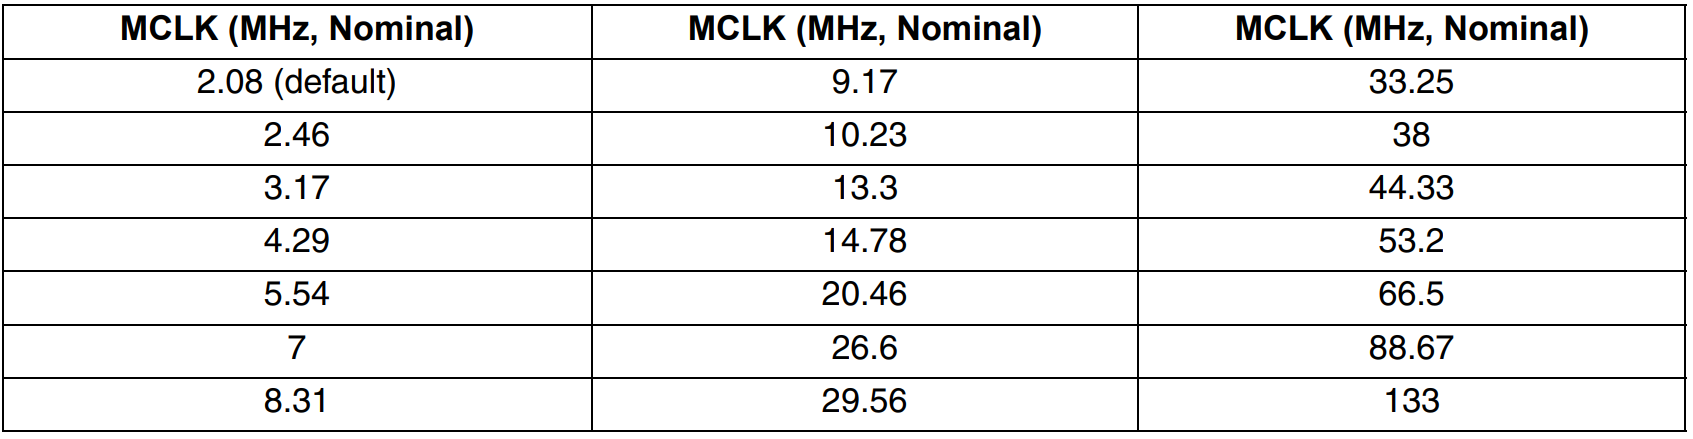
\includegraphics[trim=1mm 1mm 1mm 1mm,scale=0.344]{clkrates.PNG}
	\caption{Elérhető CLK-frekvenciák az FPGA adatlapja alapján \cite{fpgaadatlap}}
	\label{Elérhető CLK-frekvenciák az FPGA adatlapja alapján } 
\end{figure}
Az órajelet úgy kell választani, hogy elég gyors legyen, hogy a design megoldja a feladatot, amire tervezve lett. Gyorsabbra nem érdemes, mert az felesleges slack problémákhoz vezethet. 

A programozóban az órajelnek legalább 4-szer gyorsabbnak kell lennie, mint a célzott I2C órajel sebessége, mart a I2C entitás órajelenként 4 műveletet végez, és 2-szer gyorsabbnak, mint a célzott SPI órajel, mert az SPI entitás órajelenként 2 műveletet végez.


Az én célzott I2C órajel sebességem nagyobb, mint a célzott UART Baud ráta, de lassabb, 1MHz-nél. Ez azért van, mert a legtöbb modern EEPROM képes maximum 1MHz órajelsebességre, és ki szeretném használni ezt a sebességet. Ez azért kell, hogy gyorsabb legyen az I2C, mint az UART, mert az I2C tud várni az UART adatra órajel nyújtással, de a UART nem tud várni a I2C-re. Ez azért van, mert az UART sebességét  kommunikáció közben nem lehet változtatni, mert az UART aszinkron. Az SPI célsebesség pedig 5MHz körül van, hasonló okok miatt.

A programozóm UART-ot is használ, ami korábban volt tárgyalva, egy aszinkron kommunikációs protokoll. Ez azt jelenti, hogy a belső órajelet úgy kell választani, hogy jól leosztható legyen, a megcélzott Baud rátához. 

Tegyük fel, hogy a célzott Baud ráta 23040. Ha a belső órajel 2.46MHz akkor az órajelosztó számlálónak 11-ig kell számolnia, mivel \(230400$Baud$ / 2,46$MHz $ = 10,68\). Egy órajel számláló csak egész számokkal tud számolni. Így minden egyes periódus alatt fél órajelet késne a belső UART számláló, a tényleges 230400 Baud-hoz képest. Úgy kellet választanom az órajelet, hogy minimális kerekítéssel le lehessen osztania, és ez a késés a lehtő legkisseb legyen. A célzott UART sebesség 576000 Baud.

Ezek miatt választottam a 9,17MHz-t belső órajelnek. Így a UART osztó hiba 0,08 órajel per Baud periódus. A I2C maximum sebessége 2,29MHz. Az SPI Max sebessége 4,59MHz.

\subsection{A write8bit entitás}
A write8bit 8 bites adat írására szolgál az SPI vonalokon. Az entitás bemeneti és kimeneti port-jai a következők:

Port-ok:
\begin{itemize}
	\item iCS: Bemeneti vezérlőjel, amely az írási folyamat indítását jelzi ('0' értékkel aktiválódik).
	\item cs: Kimeneti vezérlőjel, amely az írási folyamat állapotát jelzi ('1' az alapértelmezett érték).
	\item Clk: Órajel bemenet, amely az állapotgép működését vezérli.
	\item Done: Kimeneti jel, amely az írási folyamat befejezését jelzi ('1' az alapértelmezett érték).
	\item bit8SCL: Órajel kimenet a soros kommunikációhoz ('1' az alapértelmezett érték).
	\item nReset: Reset bemenet, amely az állapotgépet alaphelyzetbe állítja ('0' értékkel aktiválódik).
	\item bit8SDA: Adat kimenet a soros kommunikációhoz ('1' az alapértelmezett érték).
	\item SDA\_data: 8 bites adat bemenet, amelyet a modul sorosan továbbít.
\end{itemize}
A write8bit entitás egy állapotgépet tartalmaz, amely három állapotból áll:
\begin{enumerate}
	\item Idle: Alapértelmezett állapot, ahol az órajel (bit8SCL) és az adatvonal (bit8SDA) magas szinten van, és a Done jel aktív ('1'). Ha az iCS bemenet alacsony szintre kerül ('0'), az állapotgép a write8 állapotba lép.
	\item write8: Az adat írásának állapota. Az adatot a SDA\_data bemenetről bitenként továbbítja a bit8SDA kimenetre. Az írási folyamatot a BitIndex számláló vezérli, amely 0-tól 7-ig számol. Ha az összes bitet elküldte, az állapotgép a stop állapotba lép.
	\item stop: Az írási folyamat lezárása. A cs jel visszaáll magas szintre ('1'), és az állapotgép visszatér az Idle állapotba.
\end{enumerate}
Az állapotgép működését az órajel (Clk) vezérli, és az nReset bemenet bármikor alaphelyzetbe állíthatja. A Main entitásban ez az entitás felelős az egyszerű csupán 8bites egyirányú (MOSI) SPI kommunikációkért. 
\subsection{UART\_TX entitás}
Az UART\_TX az UART protokoll szerinti adatküldést valósítja meg. Ez a modul soros adatátvitelre szolgál, ahol a bemeneti adatokat bitenként továbbítja egy kimeneti vonalon

Port-ok:
\begin{itemize}
	\item TXData: 8 bites bemeneti adat, amelyet a modul sorosan továbbít.
	\item Clk: Órajel bemenet, amely az állapotgép működését vezérli.
	\item SendTX: Bemeneti vezérlőjel, amely az adatküldés indítását jelzi ('1' értékkel aktiválódik).
	\item TXDone: Kimeneti jel, amely az adatküldés befejezését jelzi ('1' az alapértelmezett érték).
	\item nReset: Reset bemenet, amely az állapotgépet alaphelyzetbe állítja ('0' értékkel aktiválódik).
	\item TXOut: Kimeneti adatvonal, amelyen a soros adatátvitel történik.
	\item TXActive: Kimeneti jel, amely az adatküldés aktív állapotát jelzi ('1', ha a modul éppen adatot küld).
\end{itemize}
Generikus paraméter:
\begin{itemize}
	\item ClkRatio: Az órajel osztására szolgáló paraméter, amely meghatározza az UART adatátvitel sebességét (Baud rate).
\end{itemize}
A UART\_TX entitás egy állapotgépet tartalmaz, amely az UART adatküldési folyamatát valósítja meg. Az állapotgép az alábbi állapotokból áll:
\begin{enumerate}
	\item Idle: Alapértelmezett állapot, ahol a modul várakozik a SendTX jel aktiválására. Az órajel számláló (ClkCount) nullázódik, és a kimeneti vonal (TXOut) magas szinten van ('1').
	\item StartBit: Az adatküldés kezdő bitje ('0') kerül a kimeneti vonalra. Az órajel számláló növekszik, és ha eléri a ClkRatio értéket, az állapotgép a DataBits állapotba lép.
	\item DataBits: Az adatbitek soros továbbítása történik. A TXData bemenet bitjeit a BitIndex számláló segítségével küldi ki a modul. Ha az összes bit elküldésre került, az állapotgép a StopBit állapotba lép.
	\item StopBit: Az adatküldés záró bitje ('1') kerül a kimeneti vonalra. Az órajel számláló növekszik, és ha eléri a ClkRatio értéket, az állapotgép a FrameEnd állapotba lép.
	\item FrameEnd: Az adatküldés befejeződik, a TXActive jel inaktívvá válik ('0'), és a TXDone jel aktívvá válik ('1'). Az állapotgép visszatér az Idle állapotba.
\end{enumerate}
Az állapotgép működését az órajel (Clk) vezérli, és az nReset bemenet bármikor alaphelyzetbe állíthatja.

\subsection{A UART\_RX entitás}
A UART\_RX entitás az UART protokoll szerinti adatfogadást valósítja meg. Ez a modul soros adatokat fogad egy bemeneti vonalon, és azokat párhuzamos formátumba alakítja.
\begin{itemize}
	\item Clk: Órajel bemenet, amely az állapotgép működését vezérli.
	\item RXIn: Soros adat bemenet, amelyen keresztül az UART adatokat fogadja.
	\item Ack: Bemeneti vezérlőjel, amely az adatfogadás befejezésének visszaigazolására szolgál.
	\item RXData: 8 bites kimeneti adat, amely a fogadott adatot tartalmazza.
	\item RXDataReady: Kimeneti jel, amely az adatfogadás befejezését jelzi ('1' értékkel aktiválódik).
	\item nReset: Reset bemenet, amely az állapotgépet alaphelyzetbe állítja ('0' értékkel aktiválódik).
	\item RXActive: Kimeneti jel, amely az adatfogadás aktív állapotát jelzi.
\end{itemize}
Generikus paraméterek:
\begin{itemize}
	\item ClkRatio: Az órajel osztására szolgáló paraméter, amely meghatározza az UART adatátvitel sebességét (Baud rate).
	\item CRHalf: Az órajel osztásának felezett értéke, amely a bitközép detektálására szolgál.
\end{itemize}
A UART\_RX entitás egy állapotgépet tartalmaz, amely az UART adatfogadási folyamatát valósítja meg. Az állapotgép az alábbi állapotokból áll:
\begin{enumerate}
	\item Idle: Alapértelmezett állapot, ahol a modul várakozik az adatfogadás kezdetére. Ha a RXIn jel alacsony szintre kerül ('0'), az állapotgép a StartBit állapotba lép.
	\item StartBit: Az adatfogadás kezdő bitjének ('0') detektálása történik. Az órajel számláló (ClkCount) növekszik, és ha eléri a ClkRatio értéket, az állapotgép a DataBits állapotba lép.
	\item DataBits: Az adatbitek fogadása történik. A RXIn bemenet bitjeit a SData regiszterbe menti a modul, a BitIndex számláló segítségével. Ha az összes bitet fogadta, az állapotgép a StopBit állapotba lép.
	\item StopBit: Az adatfogadás záró bitjének ('1') detektálása történik. A RXDataReady jel aktívvá válik ('1'), jelezve, hogy az adat fogadása befejeződött. Ha az Ack jel aktív ('1'), az állapotgép visszatér az Idle állapotba.
\end{enumerate}
Az állapotgép működését az órajel (Clk) vezérli, és az nReset bemenet bármikor alaphelyzetbe állíthatja.
\subsection{A writePage entitás}
A writePage entitás a komplexebb SPI kommunikációkat kezeli. A neve writePage maradt, mert eredetileg a tervem az volt, hogy két entitást készítek. Egy entitást, ami az SPI írásért felelős, egy másikat ami pedig ami az olvasásért felelős. De végül egyszerűbb volt, egy entitásban megvalósítani mind két funkciót.
Ez az entitás azért is komplexebb, mert eltérően a write8bit-től képes a kommunikációs protokoll kerete hosszán állítani.

Port-ok:
\begin{itemize}
	\item iCS: Bemeneti vezérlőjel, amely az adatátviteli folyamat indítását jelzi ('0' értékkel aktiválódik).
	\item RW: Bemeneti jel, amely az írási ('0') vagy olvasási ('1') műveletet határozza meg.
	\item Rdy: Kimeneti jel, amely az adatátviteli folyamat készenlétét jelzi ('1' az alapértelmezett érték).
	\item cs: Kimeneti vezérlőjel, amely az adatátvitel állapotát jelzi ('1' az alapértelmezett érték).
	\item from\_SDO: Bemeneti adatvonal, amelyen keresztül az olvasott adat érkezik.
	\item Done: Kimeneti jel, amely az adatátviteli folyamat befejezését jelzi ('1' az alapértelmezett érték).
	\item toSCL: Órajel kimenet a soros kommunikációhoz ('1' az alapértelmezett érték).
	\item nReset: Reset bemenet, amely az állapotgépet alaphelyzetbe állítja ('0' értékkel aktiválódik).
	\item toSDA: Adat kimenet a soros kommunikációhoz ('1' az alapértelmezett érték).
	\item MISO\_DR: Kimeneti jel, amely az olvasási művelet befejezését jelzi.
	\item next8bits: 8 bites bemeneti adat, amelyet ez a entitás írni fog.
	\item read8bits: 8 bites kimeneti adat, amely az olvasott adatot tartalmazza.
	\item RW\_length: Az SPI művelet teljes hosszát meghatározó bemeneti paraméter (bájtokban).
	\item RH\_length: Az olvasási művelet címző keret hosszát meghatározó bemeneti paraméter (bájtokban).
\end{itemize}
Az állapotgép működését az órajel (Clk) vezérli, és az nReset bemenet bármikor alaphelyzetbe állíthatja.
Az állapotgép négy fő állapotot tartalmaz:

\begin{enumerate}
	\item Idle (Alapállapot) \begin{itemize}
		\item Funkció: Az állapotgép várakozik, amíg az iCS jel alacsony szintre kerül ('0'), ami az SPI kommunikáció kezdetét jelzi.
		\item Tevékenységek: \begin{itemize}
			\item Az összes kimeneti jel alaphelyzetbe állítása.
			\item Az RW jel értéke a RWlatch jelbe kerül.
			\item Ha iCS = '0', akkor: \begin{itemize}
				\item Az állapot write8-ra vált
				\item cs = '0' (chip select aktív).
				\item Done = '0' (művelet folyamatban).
				\item A next8bits bemeneti adatot a current8bits jel tárolja.
			\end{itemize}
		\end{itemize}
	\end{itemize}
	\item write8 (Írási állapot) \begin{itemize}
		\item Funkció: Az aktuális 8 bites adat (current8bits) bitenként kerül kiküldésre az SPI buszra.
		\item Tevékenységek: \begin{itemize}
			\item Az toSDA jel az aktuális bit értékét veszi fel (current8bits(7-BitIndex)).
			\item Az toSCL jel váltakozik ('0' → '1'), hogy az órajelet biztosítsa.
			\item A BitIndex növekszik minden bit kiküldése után.
			\item Ha az összes bit kiküldésre került (BitIndex = 7), akkor: \begin{itemize}
				\item Az állapot stop-ra vált.
				\item A BitIndex alaphelyzetbe kerül.
			\end{itemize}
		\end{itemize}
	\end{itemize}
	\item read8 (Olvasási állapot) \begin{itemize}
		\item Funkció: Az SPI buszról érkező adatot bitenként olvassa be.
		\item Tevékenységek: \begin{itemize}
			\item Az toSCL jel váltakozik ('0' → '1'), hogy az órajelet biztosítsa.
			\item Az from\_SDO bemeneti jel értéke a read8bits jel megfelelő bitjébe kerül (read8bits(7-BitIndex)).
			\item A BitIndex növekszik minden bit beolvasása után.
			\item Ha az összes bit beolvasásra került (BitIndex = 7), akkor: \begin{itemize} 
			\item Az állapot stop-ra vált.
			\item A MISO\_DR jel '1'-re áll, jelezve, hogy az adat érvényes.
			\end{itemize}
		\end{itemize}
	\end{itemize}
	\item stop (Befejezési állapot) \begin{itemize}
		\item Itt történik az állapotok közötti váltási logika az iCS, RW, BitIndex, és ByteIndex jelek alapján. Mindig várja az iCS jel alacsony szintjét, mielőtt állapotot vált. Ha a RWlatch = ’1’, akkor felelős annak ellenőrzéséért, hogy az SPI üzenet elérte-e a megadott fejléc hosszúságát. Ha igen, akkor write8 helyett read8-be ugrik. Illetve, ha az üzenet elérte a teljes hosszát, visszatér az Idle állapotba.
	\end{itemize}
\end{enumerate}
\subsection{A I2C entitás}
Az I2C entitás az I2C protokoll szerinti adatátvitelt valósítja meg. Ez az entitás képes adatokat írni és olvasni egy I2C buszon, és támogatja a protokollhoz szükséges vezérlőjelek generálását. Ez az entitás is komplex, képes írni és olvasni, és a kommunikációs protokoll kerete hosszán állítani.

Port-ok:
\begin{itemize}
	\item DataIn: 8 bites bemeneti adat, amelyet a modul az I2C buszra ír.
	\item DataOut: 8 bites kimeneti adat, amely az I2C buszról olvasott adatot tartalmazza.
	\item RW\_length: Az írási művelet hosszát meghatározó bemeneti paraméter (bájtokban).
	\item RH\_length: Az olvasási művelet címző keret hosszát meghatározó bemeneti paraméter (bájtokban).
	\item Clk: Órajel bemenet, amely az állapotgép működését vezérli.
	\item Go: Bemeneti vezérlőjel, amely az I2C művelet indítását jelzi.
	\item Send\_i2c: Bemeneti jel, amely az I2C adatátvitel indítását szabályozza.
	\item nReset: Aszinkron reset bemenet, amely az állapotgépet alaphelyzetbe állítja ('0' értékkel aktiválódik).
	\item RW: Bemeneti jel, amely az írási ('0') vagy olvasási ('1') műveletet határozza meg.
	\item rSDA: Kétirányú adatvonal az I2C buszhoz.
	\item rSCL: Órajel kimenet az I2C buszhoz.
	\item dataready: Kimeneti jel, amely az adatátvitel befejezését jelzi.
	\item atstop: Kimeneti jel, amely az I2C stop feltétel elérését jelzi.
	\item Done: Kimeneti jel, amely az I2C művelet befejezését jelzi.
\end{itemize}
A célzott órajel sebesség, mint előbb is említettem, 576kHz és 1MHz között van. A belső órajel 9.17MHz, így 15-tel leosztva az I2C órajel 661kHz.

Állapotok Leírása:
\begin{itemize}
	\item off \begin{itemize}
		\item Cél: Ez az alapértelmezett, nyugalmi állapot, ahol az I2C modul várakozik az indító jelre.
		\item Műveletek: Az összes belső számláló (Bitcount, Bytecount, count) és retesz (RWlatch, dataready) alaphelyzetbe állítása.
		\item Átmenet: Send\_i2c = '1' esetén az állapot start-ra vált.
	\end{itemize}
	\item start \begin{itemize}
		\item Cél: Az I2C start feltétel generálása.
		\item Műveletek: \begin{itemize}
			\item A SDAen és SCLen jelek váltogatása a start feltétel létrehozásához.
			\item A count jel növelése az időzítés nyomon követésére.
		\end{itemize}
		\item Átmenet: 15 órajelciklus után az állapot PFHW-ra vált.
	\end{itemize}

	 \item PFHW (Packet Frame Header and Write):
    \begin{itemize}
        \item Cél: Az adatcsomag fejlécének és az adat bájtok biten ként való továbbítása.
        \item Műveletek:
        \begin{itemize}
            \item A SDAen jel meghajtása a DataIn aktuális bitjével.
            \item A SCLen váltogatása órajelek generálásához.
            \item A bit- és bájtszámlálók (Bitcount, Bytecount) nyomon követése.
        \end{itemize}
        \item Átmenet:
        \begin{itemize}
            \item 8 bit (1 bájt) továbbítása után az állapot wack-ra vált.
            \item Több bájt esetén a Bytecount növekszik.
        \end{itemize}
    \end{itemize}
    \item wack (Write Acknowledge):
    \begin{itemize}
        \item Cél: Az írási művelet után a szolga eszköz visszaigazolásának (ACK) várakozása.
        \item Műveletek:
        \begin{itemize}
            \item A SDAen jel '1' értékre állítása, az SDA vonal felszabadításához.
            \item A SCLen váltogatása, órajelek generálásához.
            \item A golatch jel ellenőrzése, a következő művelet meghatározásához.
        \end{itemize}
        \item Átmenet:
        \begin{itemize}
            \item Ha golatch = '1', az állapot PFHW-ra vált további adatátvitelhez.
            \item Ha az írási művelet befejeződött (Bytecount = RW\_length), az állapot stop-ra vált.
            \item Ha olvasási műveletre váltás történik (Bytecount >= RH\_length), az állapot readB-re vált.
        \end{itemize}
    \end{itemize}
    \item readB (Read Byte):
    \begin{itemize}
        \item Cél: Egy bájt adat olvasása a szolga eszközről.
        \item Műveletek:
        \begin{itemize}
            \item A SDAen jel '1' értékre állítása az SDA vonal felszabadításához.
            \item Az rSDA értékének rögzítése a DataOut jelbe a 8. órajelciklus alatt.
            \item A SCLen váltogatása órajelek generálásához.
            \item A bit- és bájtszámlálók (Bitcount, Bytecount) nyomon követése.
        \end{itemize}
        \item Átmenet:
        \begin{itemize}
            \item 8 bit (1 bájt) olvasása után az állapot rack-ra vált.
        \end{itemize}
    \end{itemize}
    \item rack (Read Acknowledge):
    \begin{itemize}
        \item Cél: Visszaigazolás (ACK) küldése a szolga eszköznek az olvasási művelet után.
        \item Műveletek:
        \begin{itemize}
            \item A SDAen jel '0' értékre állítása ACK küldéséhez, vagy '1' értékre NACK küldéséhez (ha az olvasási művelet befejeződött).
            \item A SCLen váltogatása órajelek generálásához.
            \item A golatch jel ellenőrzése a következő művelet meghatározásához.
        \end{itemize}
        \item Átmenet:
        \begin{itemize}
            \item Ha golatch = '1', az állapot readB-re vált további adatfogadáshoz.
            \item Ha az olvasási művelet befejeződött (Bytecount = RW\_length), az állapot stop-ra vált.
        \end{itemize}
    \end{itemize}
    \item restart:
    \begin{itemize}
        \item Cél: Ismételt start feltétel generálása több részből álló tranzakciókhoz.
        \item Műveletek:
        \begin{itemize}
            \item A SDAen és SCLen váltogatása az ismételt start feltétel létrehozásához.
            \item A count jel alaphelyzetbe állítása.
        \end{itemize}
        \item Átmenet: 15 órajelciklus után az állapot PFHW-ra vált.
    \end{itemize}
    \item stop:
    \begin{itemize}
        \item Cél: Az I2C stop feltétel generálása a kommunikáció befejezéséhez.
        \item Műveletek:
        \begin{itemize}
            \item A SDAen és SCLen váltogatása a stop feltétel létrehozásához.
            \item Az összes belső számláló (count, Bytecount) alaphelyzetbe állítása.
            \item A dataready jel '0' értékre állítása.
        \end{itemize}
        \item Átmenet: 15 órajelciklus után az állapot off-ra vált.
    \end{itemize}

\end{itemize}
\section{A main (fő) entitás}
A main entitás biztosítja a programozó funkcionalitását, az összes alentitást használva. A felhasználó által küldött utasításokat értelmezi, és az USB-n keresztül küldött adatfolyamot továbbítja a I2C és SPI alentitásoknak. Azért is felelős, hogy a I2C és SPI adatfolyamok szinkronizálva maradjanak az UART adatfolyamatok. 
\subsection{A main entitás állapotgép}
\begin{itemize}
    \item 000 (Base State):
    \begin{itemize}
        \item Cél: Az alapállapot, ahol a rendszer várakozik a bemeneti jelre.
        \item Műveletek:
        \begin{itemize}
            \item Az összes vezérlőjel alaphelyzetbe állítása.
            \item Ha az UART fogadási művelet befejeződött, az állapot a StateHolder értékére vált.
        \end{itemize}
        \item Átmenet: Az UART fogadási művelet (RXDR) és az SPI írási művelet (DoneW) befejeződése után.
    \end{itemize}
    \item 001 (SPI Configure):
    \begin{itemize}
        \item Cél: Egy bájtos SPI kommunikációk végrehajtása.
        \item Műveletek:
        \begin{itemize}
            \item Az SPI vonalak vezérlése a write8bit modul segítségével.
            \item Az UART fogadási adatainak (DataFromRx) továbbítása az SPI modul felé.
        \end{itemize}
        \item Átmenet: Az SPI művelet befejezése után visszatérés az alapállapotba.
    \end{itemize}
    \item 010 (SPI Read):
    \begin{itemize}
        \item Cél: Az SPI olvasási művelet végrehajtása.
        \item Műveletek:
        \begin{itemize}
            \item Az SPI olvasási művelet indítása a writePage modul segítségével.
            \item Az olvasott adat (SDO\_datap) továbbítása az UART felé.
        \end{itemize}
        \item Átmenet: Az SPI olvasási művelet befejezése után visszatérés az alapállapotba.
    \end{itemize}
    \item 011 (SPI Write):
    \begin{itemize}
        \item Cél: Az SPI írási művelet végrehajtása.
        \item Műveletek:
        \begin{itemize}
            \item Az SPI írási művelet indítása a writePage modul segítségével.
            \item Az UART fogadási adatainak (DataFromRx) továbbítása az SPI modul felé.
        \end{itemize}
        \item Átmenet: Az SPI írási művelet befejezése után visszatérés az alapállapotba.
    \end{itemize}
    \item 100 (Get Settings):
    \begin{itemize}
        \item Cél: A rendszer konfigurációs beállításainak frissítése.
        \item Műveletek:
        \begin{itemize}
            \item Az UART fogadási adatainak (DataFromRx) tárolása a settings vektorban.
        \end{itemize}
        \item Átmenet: A settings vektor feltöltése után visszatérés az alapállapotba.
    \end{itemize}
    \item 101 (I2C Read):
    \begin{itemize}
        \item Cél: Az I2C olvasási művelet végrehajtása.
        \item Műveletek:
        \begin{itemize}
            \item Az I2C olvasási művelet indítása az I2C modul segítségével.
            \item Az olvasott adat (i2c\_DataOut) továbbítása az UART felé.
        \end{itemize}
        \item Átmenet: Az I2C olvasási művelet befejezése után visszatérés az alapállapotba.
    \end{itemize}
    \item 110 (I2C Write):
    \begin{itemize}
        \item Cél: Az I2C írási művelet végrehajtása.
        \item Műveletek:
        \begin{itemize}
            \item Az I2C írási művelet indítása az I2C modul segítségével.
            \item Az UART fogadási adatainak (DataFromRx) továbbítása az I2C modul felé.
        \end{itemize}
        \item Átmenet: Az I2C írási művelet befejezése után visszatérés az alapállapotba.
    \end{itemize} 
\end{itemize}
\section{C++-ban megírt utasítás küldő program}
\subsection{A "Terminal app" program}
A program célja, hogy hexadecimális formátumban megadott adatokat küldjön a számítógéphez csatlakoztatott programozónak egy COM soros port-on keresztül, majd fogadja és megjelenítse a programozótól visszakapott adatokat.
\subsubsection{A program működése}
\begin{enumerate}
	\item Soros port megnyitása és beállítása.
\begin{itemize}
	\item A program a "CreateFile" függvénnyel megnyitja a COM port-ot olvasásra és írásra.
	\item A "SetupComm" függvénnyel 1 MB-os bemeneti és kimeneti puffert állít be a soros port-hoz.
	\item A DCB struktúrában beállítja a kommunikációs paramétereket. Például: Baud ráta: 576000, 8 adatbit, 1 stopbit, és paritás bit nélküli adatkeret.
	\item A COMMTIMEOUTS struktúrában beállítja az időzítéseket az olvasáshoz és íráshoz.
\end{itemize}
	\item Felhasználói adatbekérés és feldolgozás.
\begin{itemize}
	\item A program egy végtelen ciklusban várja a felhasználó bemenetét.
	\item A felhasználó hexadecimális karakterláncot írhat be (például: AABBCC), vagy az exit szót a kilépéshez.
	\item Az üres sorokat figyelmen kívül hagyja.
	\item A beírt hexadecimális karakterláncot bájt tömbbé alakítja (két karakter = 1 bájt).
\end{itemize}
	\item Adatküldés a programozónak.
\begin{itemize}
	\item Az adatokat 4096 bájtos (4 KB) blokkokban küldi el a soros port-on keresztül.
	\item Minden elküldött blokk után kiírja, hány bájtot sikerült elküldeni.
\end{itemize}
	\item Válasz fogadása a programozótól.
\begin{itemize}
	\item 50ms várakozás után lekérdezi, mennyi adat érkezett vissza a soros port bemeneti pufferébe.
	\item A beérkezett adatokat szintén 4096 bájtos blokkokban olvassa be.
	\item Az olvasott adatokat hexadecimális formátumban jeleníti meg a képernyőn.
\end{itemize}
\end{enumerate}
\subsection{A "File app" program}
Ez a program hasonló a Terminal app-hoz, de fájlokkal dolgozik. A felhasználó megadhat egy fájlnevet, amely utasításokat tartalmaz. A fájlban lévő utasításokat a program feldolgozza, és a válaszokat kiírja, és lementi egy log.txt fájlba.
\subsection{A programozó beállítása a belső memória segítségével}
A programozónak van egy 7 bájtos belső memóriája, ahol a SPI és I2C adatkeret beállításokat tárolja. Az alapértelmezett értéke x00001904000403. 

Az elő 3 bajt, azaz alapból a x000019, A SPI adatkeret teljes hosszát (bájtokban) határozza meg, U3 adattipúsban. Így alapértelmezett esetben a SPI kommunikáció teljes hossza 25 bájt. 

A következő 2 bájt pedig a SPI olvasás esetén az olvasási fejléc hossza U1 adattípusban. Alapértelmezett esetben 4 bájt a hossz. 

A következő 4 bájt pedig a I2C adatkeret teljes hosszát (bájtokban) határozza meg, U2 adattipúsban. Alapértelmezett esetben 4 bájt a hossz.

Az utolsó 2 bájt pedig a I2C olvasás esetén az olvasási fejléc hossza U1 adattípusban. Alapértelmezett esetben 3 bájt a hossz.

Tegyük fel, hogy egy SPI olvasást, és egy I2C olvasást akarunk végrehajtani. Mégpedig egy teljes page olvasást a W25Q64JV SPI Flash-ből, és egy 4 bájtos olvasást szeretnénk az AT24C256 EEPROM-ból. 

A page hossza összesen 256B, egy darab utasításbájtnak kell lenni, és három címbájtnak \cite{FLASH}. Tehát a teljes adatkeret hossz 260B bájt lesz, és az olvasási fejléc hossza 4 bájt \cite{EEPROM}. Választott címen való olvasáshoz 4 fejlécbájt kell az EEPROM-nak. Így a beállítás belső memóriát x00010404000804 re kell állítani.

Ezzel az utasítás tudjuk ezt beállítani: 4400010404000804.

Az első bájt a programozót a megfelelő "get setting” állapotba billenti. Az utasítás többi része az, amit be akarunk írni a belső memóriába. 

Az utasítás után a programozó automatikusan visszakerül az "Idle” alapállapotba.

\subsection{Utasítások és utasítássor példa és magyarázat.}
Mint korábban említettem, a programozónak összesen 7 fő állapota van. Az alap állapot a base state. Ebből az állapotból, 6 másik állapotba lehet lépni. 
Minden utasítás első bájtja, azaz első két hexadecimális karaktere, azt határozza meg, hogy melyik állapotba lépjen a programozó.
Az állapotok és hozzájuk tartozó hexadecimálisan kifejezett bájt:
\begin{table}[H]
\centering 
\begin{tabular}{lllll}
\textbf{Állapot}                      & \textbf{Hexadecimális kód}            & \textbf{Ascii kód}        &  &  \\
\cellcolor[HTML]{D9D9D9}SPI configure & \cellcolor[HTML]{D9D9D9}41 & \cellcolor[HTML]{D9D9D9}A &  &  \\
SPI read                              & 42                         & B                         &  &  \\
\cellcolor[HTML]{D9D9D9}SPI write     & \cellcolor[HTML]{D9D9D9}43 & \cellcolor[HTML]{D9D9D9}C &  &  \\
Get settings                          & 44                         & D                         &  &  \\
\cellcolor[HTML]{D9D9D9}I2C read      & \cellcolor[HTML]{D9D9D9}45 & \cellcolor[HTML]{D9D9D9}E &  &  \\
I2C write                             & 46                         & F                         &  & 
\end{tabular}
\caption{Állapotokhoz tartozó hexadecimális kódok}.
\label{Állapotokhoz tartozó hexadecimális kódok} 
\end{table}

\chapter{Tesztelés}

\section{Tesztelési elrendezés és analízis}
A projekt során egy logikai analizátort használtam. A logikai analizátor egy olyan eszköz, amely lehetővé teszi a digitális jelek időbeli viselkedésének megfigyelését, és elemzését. Az analizátor képes rögzíteni, és megjeleníteni a digitális jelek állapotát, lehetővé téve a tervezők számára, hogy megértsék a rendszer működését és hibáit. Rendkívül hasznos volt a hibakeresésre.

Egy Sealeae logic 24MS/s-es logikai analizátort használtam. És 2 memória modult is, egy I2C EEPROM-ot, és egy SPI Flash-t, hogy ellenőrizni tudjam programozó működését.

A I2C EEPROM cikkszáma: AT24C256. Egy 256Kb-es EEPROM \cite{EEPROM}

A SPI Flash cikkszáma W25Q64FV. Egy 64Mb-es Flash \cite{FLASH}

A tesztelés és analízis és a mérési elrendezés breadboard-on történt, mert a nyákon nem lehet egyszerre csatlakoztatni a memória modulokat, és az analizátort is.

Az elrendezés:
\begin{figure}[H]
	\centering
	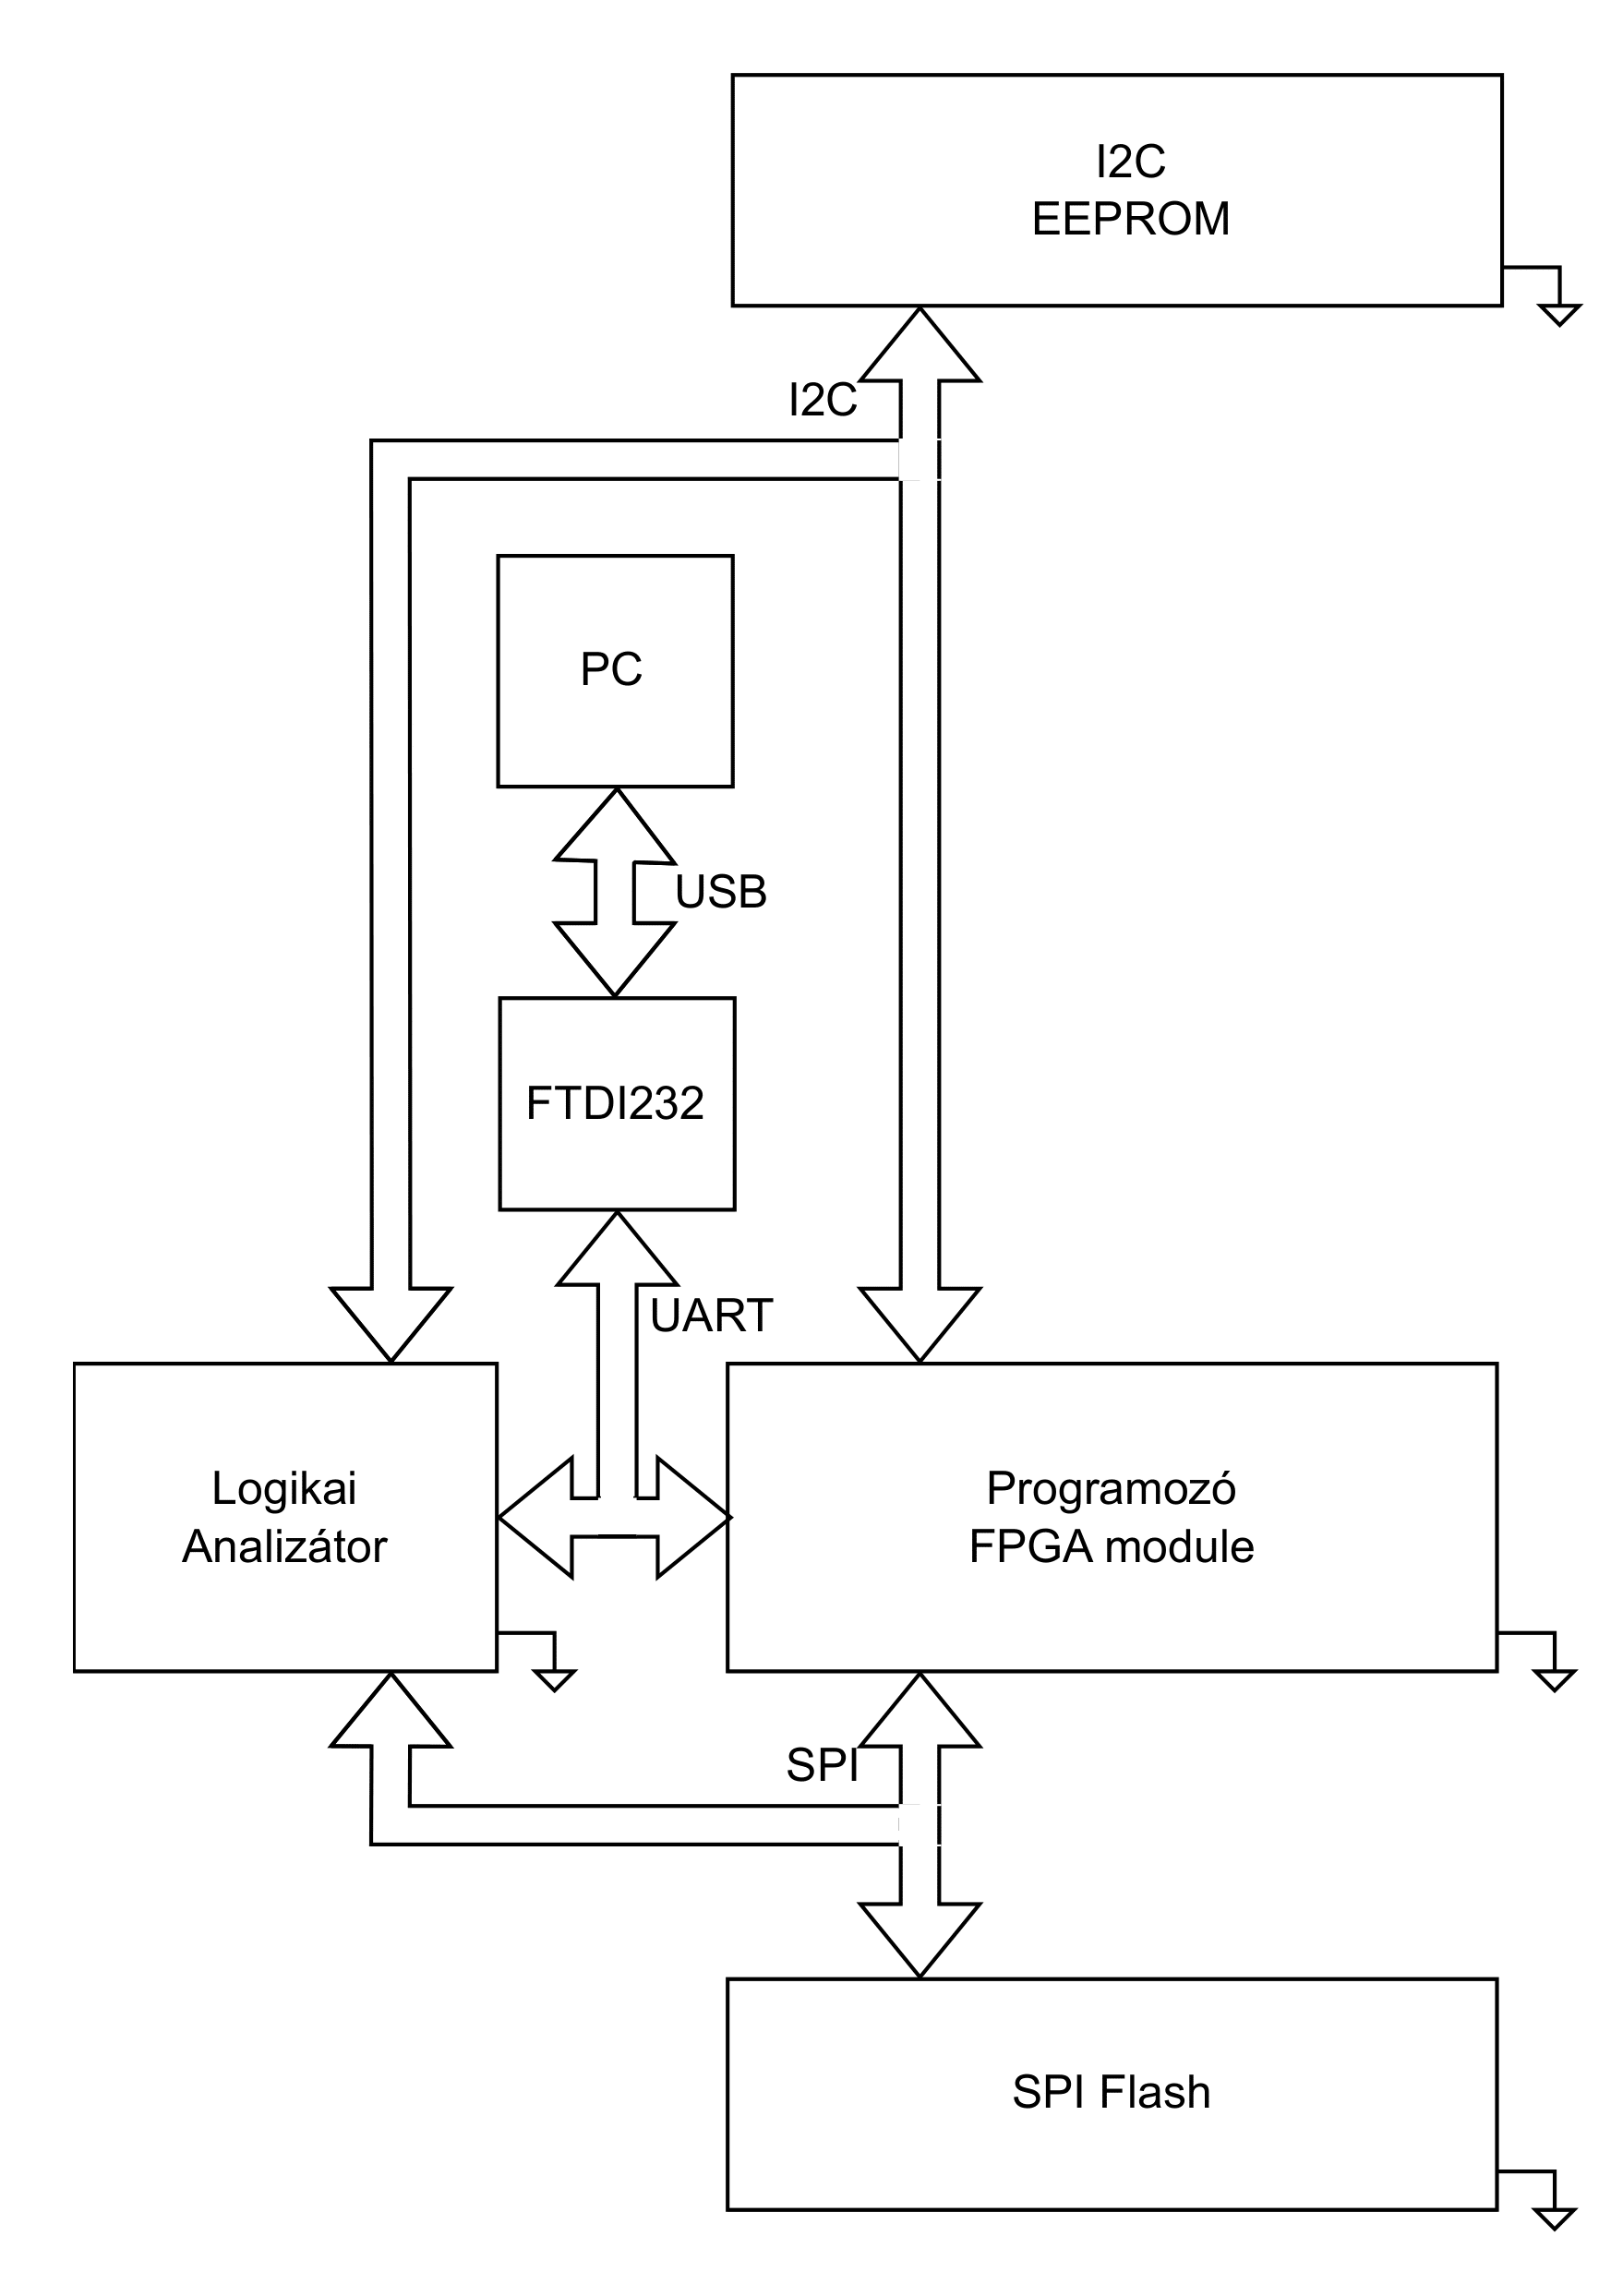
\includegraphics[trim=1mm 1mm 1mm 1mm,scale=0.14]{setupblock.PNG}
	\caption{Analízis elrendezés blokkvázlata}
	\label{Analízis elrendezés blokkvázlata}
\end{figure}
\begin{figure}[H]  
	\centering
	\includegraphics[trim=1mm 1mm 1mm 1mm,scale=0.11]{setupreal.PNG}
	\caption{Analízis elrendezés breadboard-on}
	\label{Analízis elrendezés breadboard-on}
\end{figure}

\section{Tesztelés}
\subsection{SPI configure állapot tesztelése}
Az SPI configure mindig egybájtos SPI írás, a programozó beállításaitól függetlenül. Ezt az állapotot azért hoztam létre, hogy egybájtos utasításokat könnyen tudjak írni, mint például a "chip erase", vagy "write enable". \cite{FLASH}

Teszteléshez is "write enable" utasítást küldök a SPI Flash memóriának.
A Használt utasítássor az utasítás fájlban: 

4106

exit

\subsubsection{A teszt eredménye:}


Log fájl tartalma:

Bytes written: 2

Bytes in queue: 1

Received: 41

\subsubsection{Rögzítés:}

\begin{figure}[H]  
	\centering
	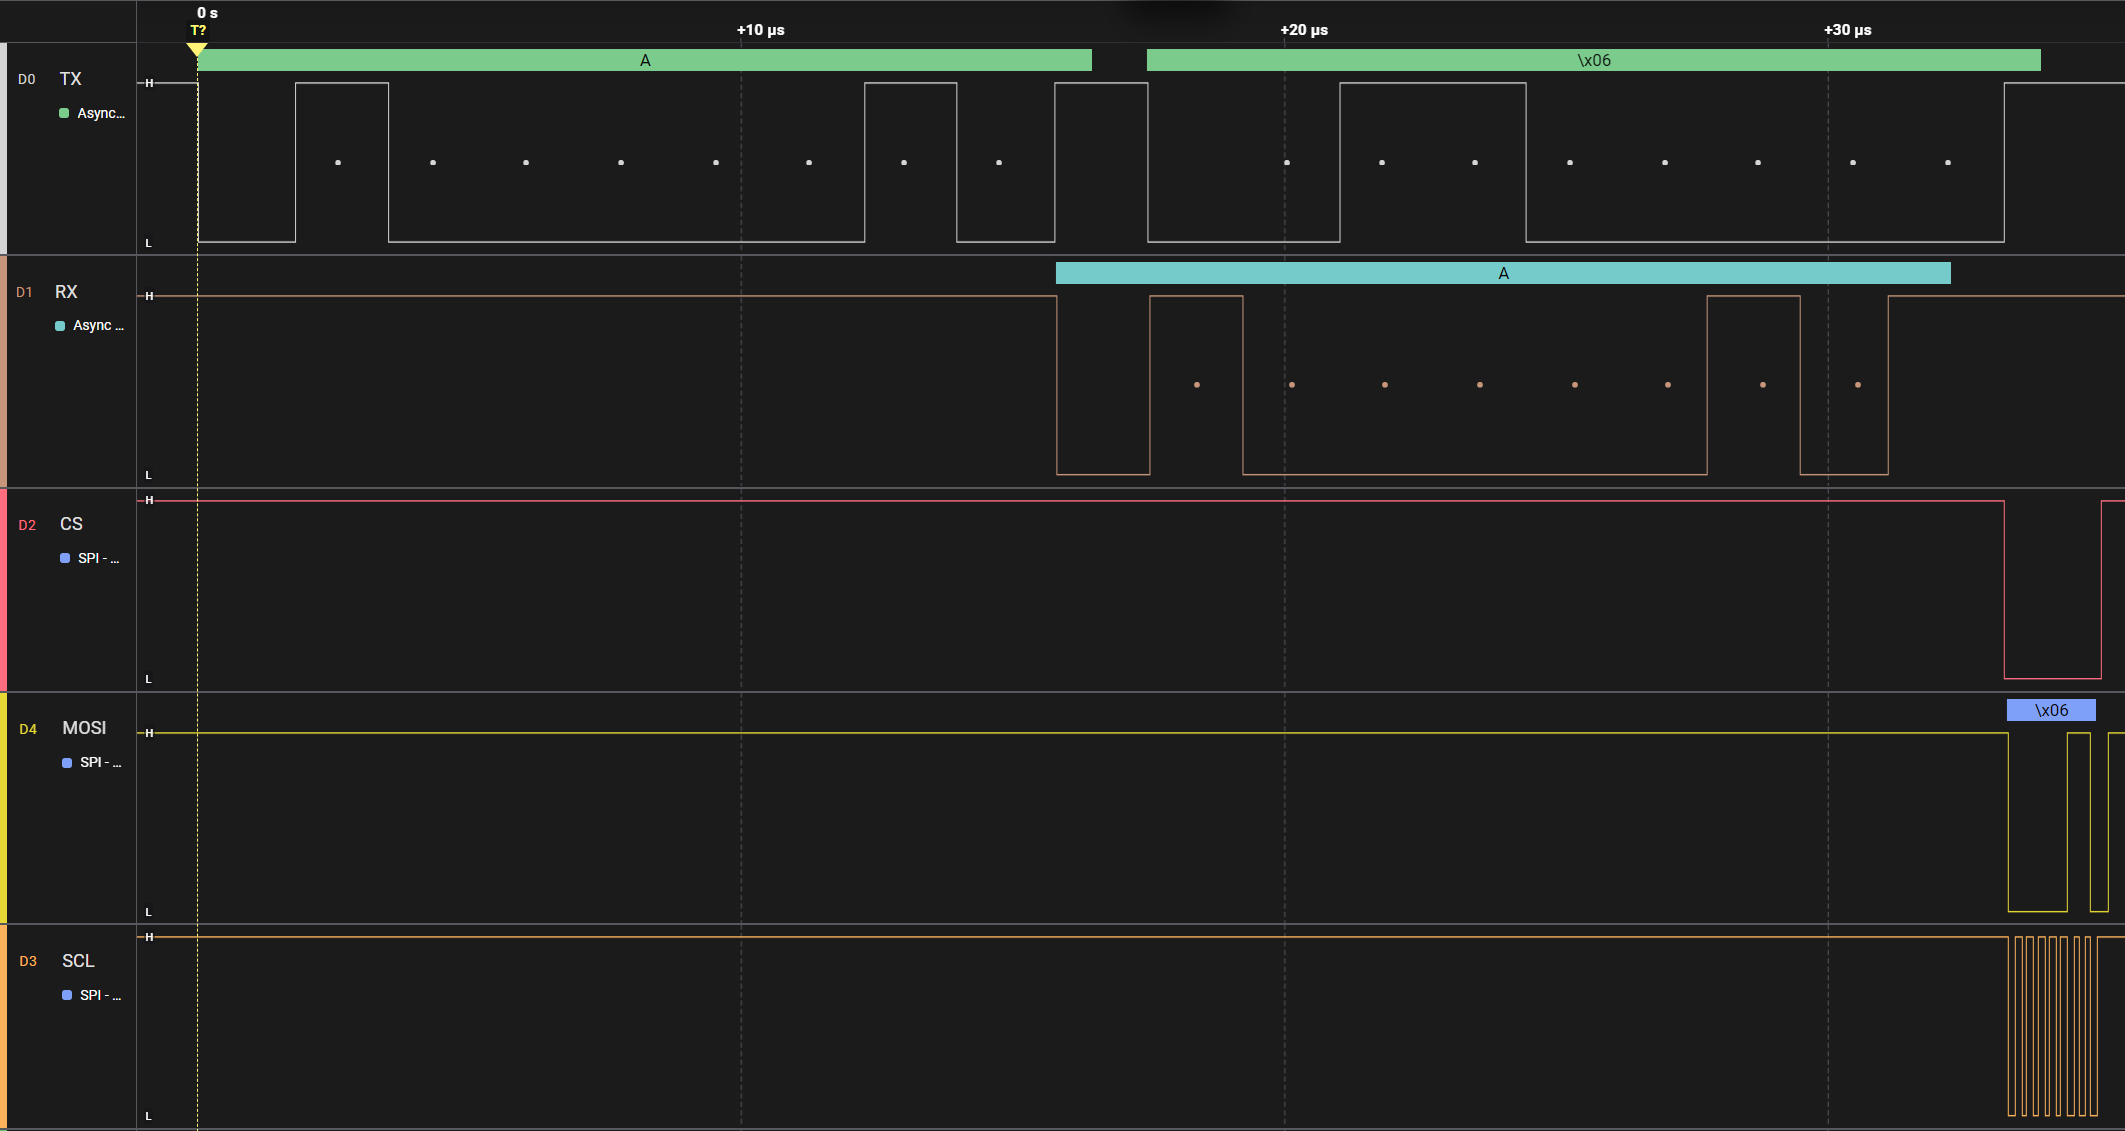
\includegraphics[trim=1mm 1mm 1mm 1mm,scale=0.25]{spiconfiguretest.PNG}
	\caption{SPI configure állapot tesztelése}
	\label{SPI configure állapot tesztelése}
\end{figure}

A képen látható, hogy a programozó fogadja a x42 értékű bájtot, és visszaküldi. A következő bájtot már viszont SPI-on írja. Ugyanazt írja SPI-on, mint amit kapott UART-on. 

Az SPI configure állapot megfelelően működik.

\subsection{SPI write állapot tesztelése}
Teszteléshez az SPI Flash memóriában egy teljes page-et azaz oldalt írtam. Ez 256 bájtnyi adat, a legtöbb, amit egy kommunikációval lehet írni az SPI Flash-be \cite{FLASH}.


A Használt utasítássor az utasítás fájlban:

4400010404000504

4106

\wrapletters{43020000004163636F7264696E6720746F20616C6C206B6E6F776E206C617773206F66206176696174696F6E2C207468657265206973206E6F207761792061206265652073686F756C642062652061626C6520746F20666C792E204974732077696E67732061726520746F6F20736D616C6C20746F206765742069747320666174206C6974746C6520626F6479206F6666207468652067726F756E642E20546865206265652C206F6620636F757273652C20666C69657320616E797761792062656361757365206265657320646F6E2774206361726520776861742068756D616E73207468696E6B20697320696D706F737369626C652E2059656C6C6F772C20626C61636B0}

exit


Az első két utasítás azért kell, hogy beállítsuk a SPI kommunikáció hosszát és az Flash-nek elküldjük a "write enable" utasítást. Maga az adat, a harmadik utasításban van. És a "Bee Movie" film forgatókönyvének első 256 bájtja.

\subsubsection{A teszt eredménye:}

Log fájl tartalma:

Bytes written: 8

Bytes in queue: 1

Received: 44 

Bytes written: 2

Bytes in queue: 1

Received: 41 

Bytes written: 262

Bytes in queue: 1

Received: 43


\subsubsection{Rögzítés:}


\begin{figure}[H]  
	\centering
	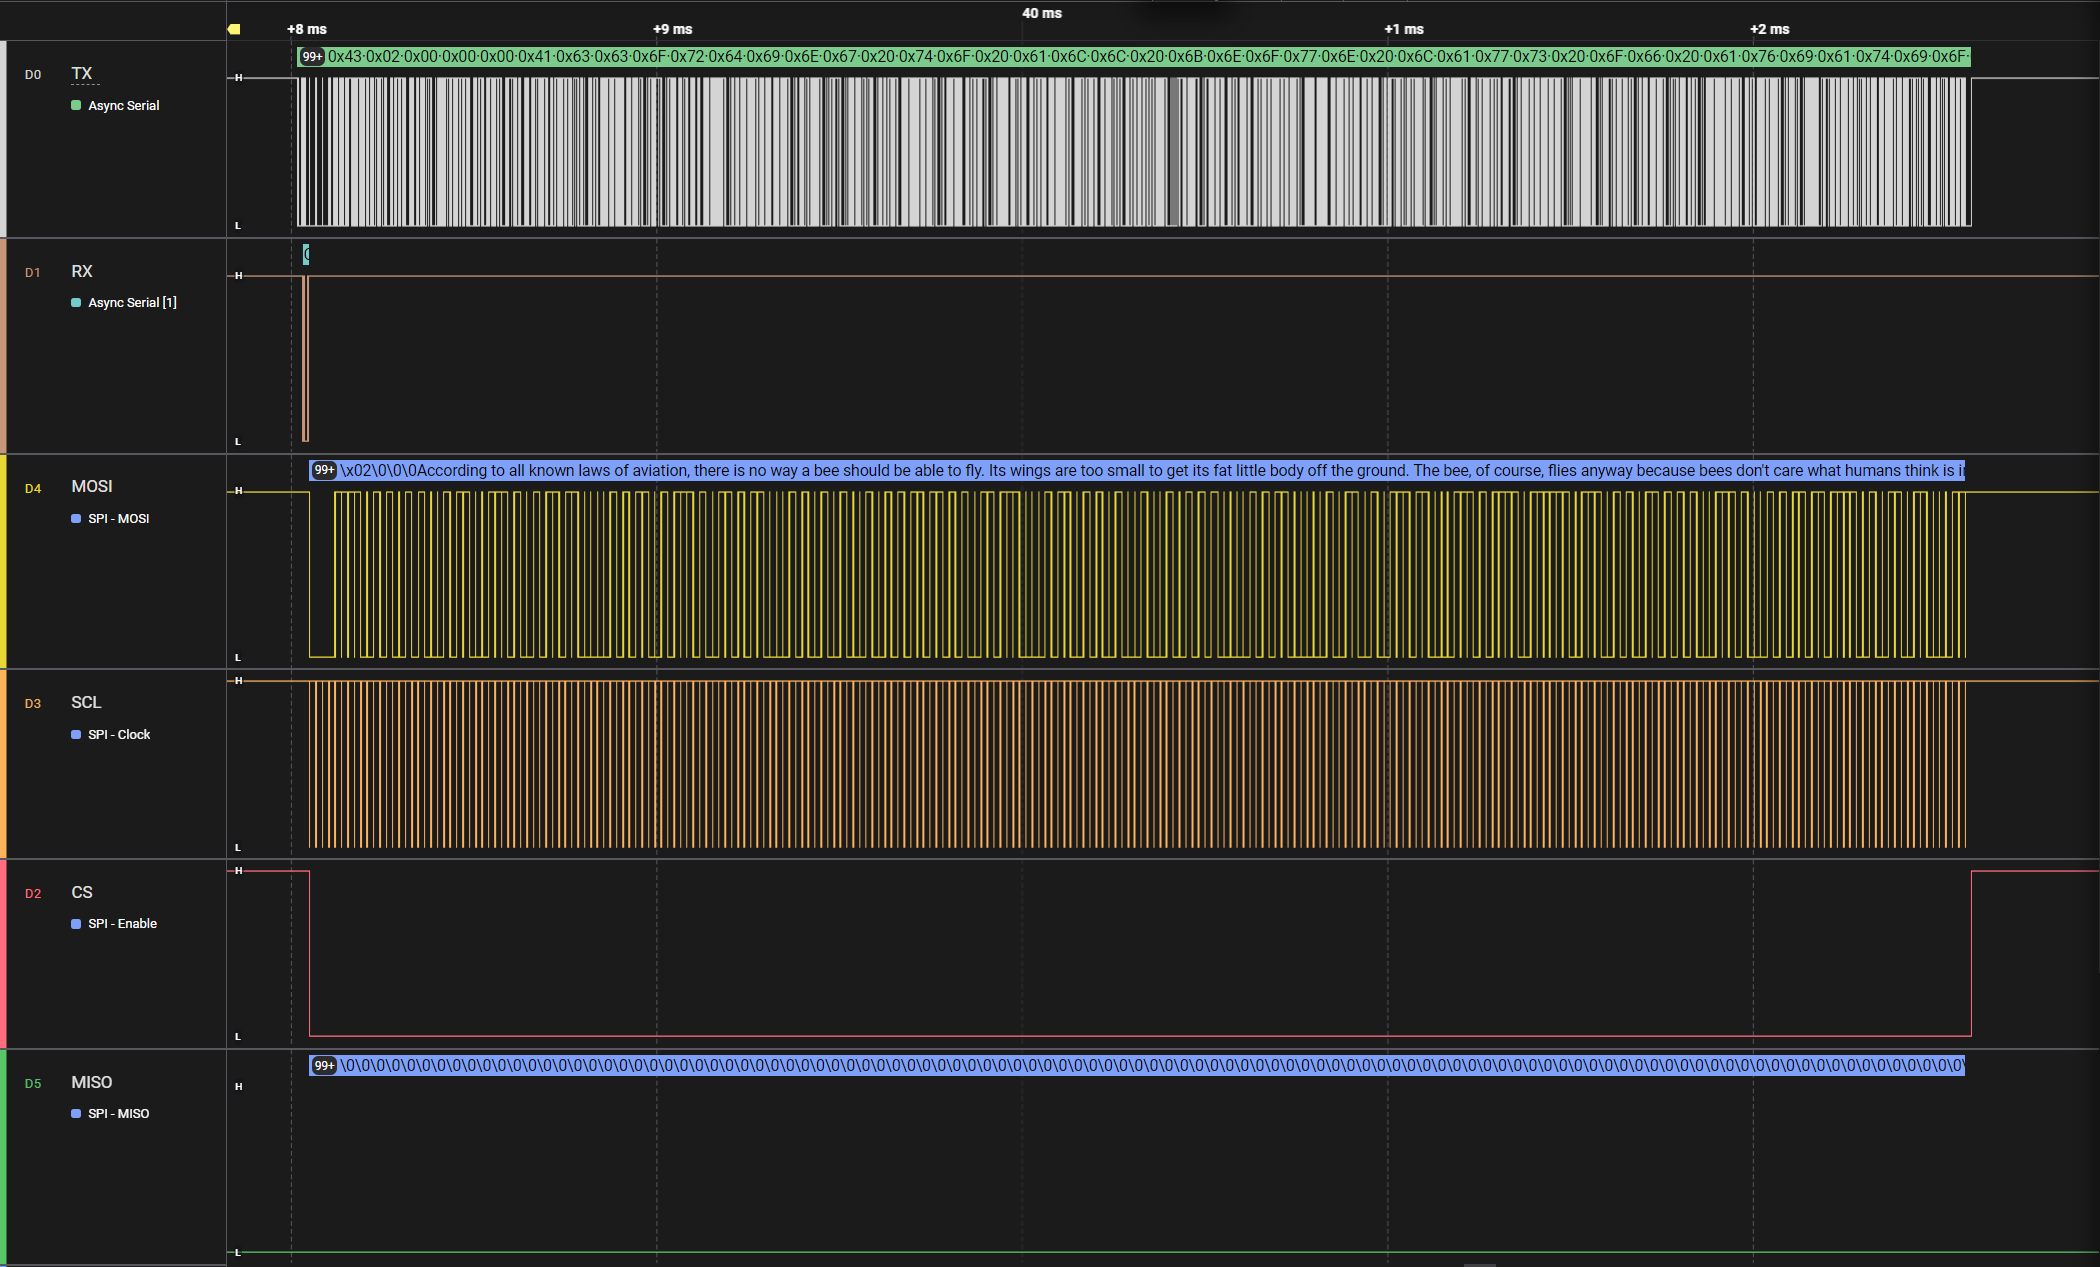
\includegraphics[trim=1mm 1mm 1mm 1mm,scale=0.28]{spi write packege full.PNG}
	\caption{SPI write állapot tesztelése}
	\label{SPI write állapot tesztelése}
\end{figure}

A képen látszik, hogy az programozó valóban az összes érkező bájtot helyesen elküldi a Flash-nek SPI-on keresztül. 

Az SPI write állapot megfelelően működik.

\subsection{SPI read állapot tesztelése}

Teszteléshez az SPI Flash memóriában egy teljes page-et, azaz oldalt olvastam ki. Ugyan azt, amit beleírtam az SPI write tesztelés közben.

A Használt utasítássor az utasítás fájlban:

4400010404000504

42030000000

Itt is az első utasítás azért kell, hogy beállítsuk a SPI kommunikáció hosszát. 

\subsubsection{A teszt eredménye:}

Log fájl tartalma:

Bytes written: 8

Bytes in queue: 1

Received: 44 

Bytes written: 6

Bytes in queue: 257

Received: 41 63 63 6F 72 (...többi adat bájt...) 36 B0

\subsubsection{Rögzítés:}


\begin{figure}[H]  
	\centering
	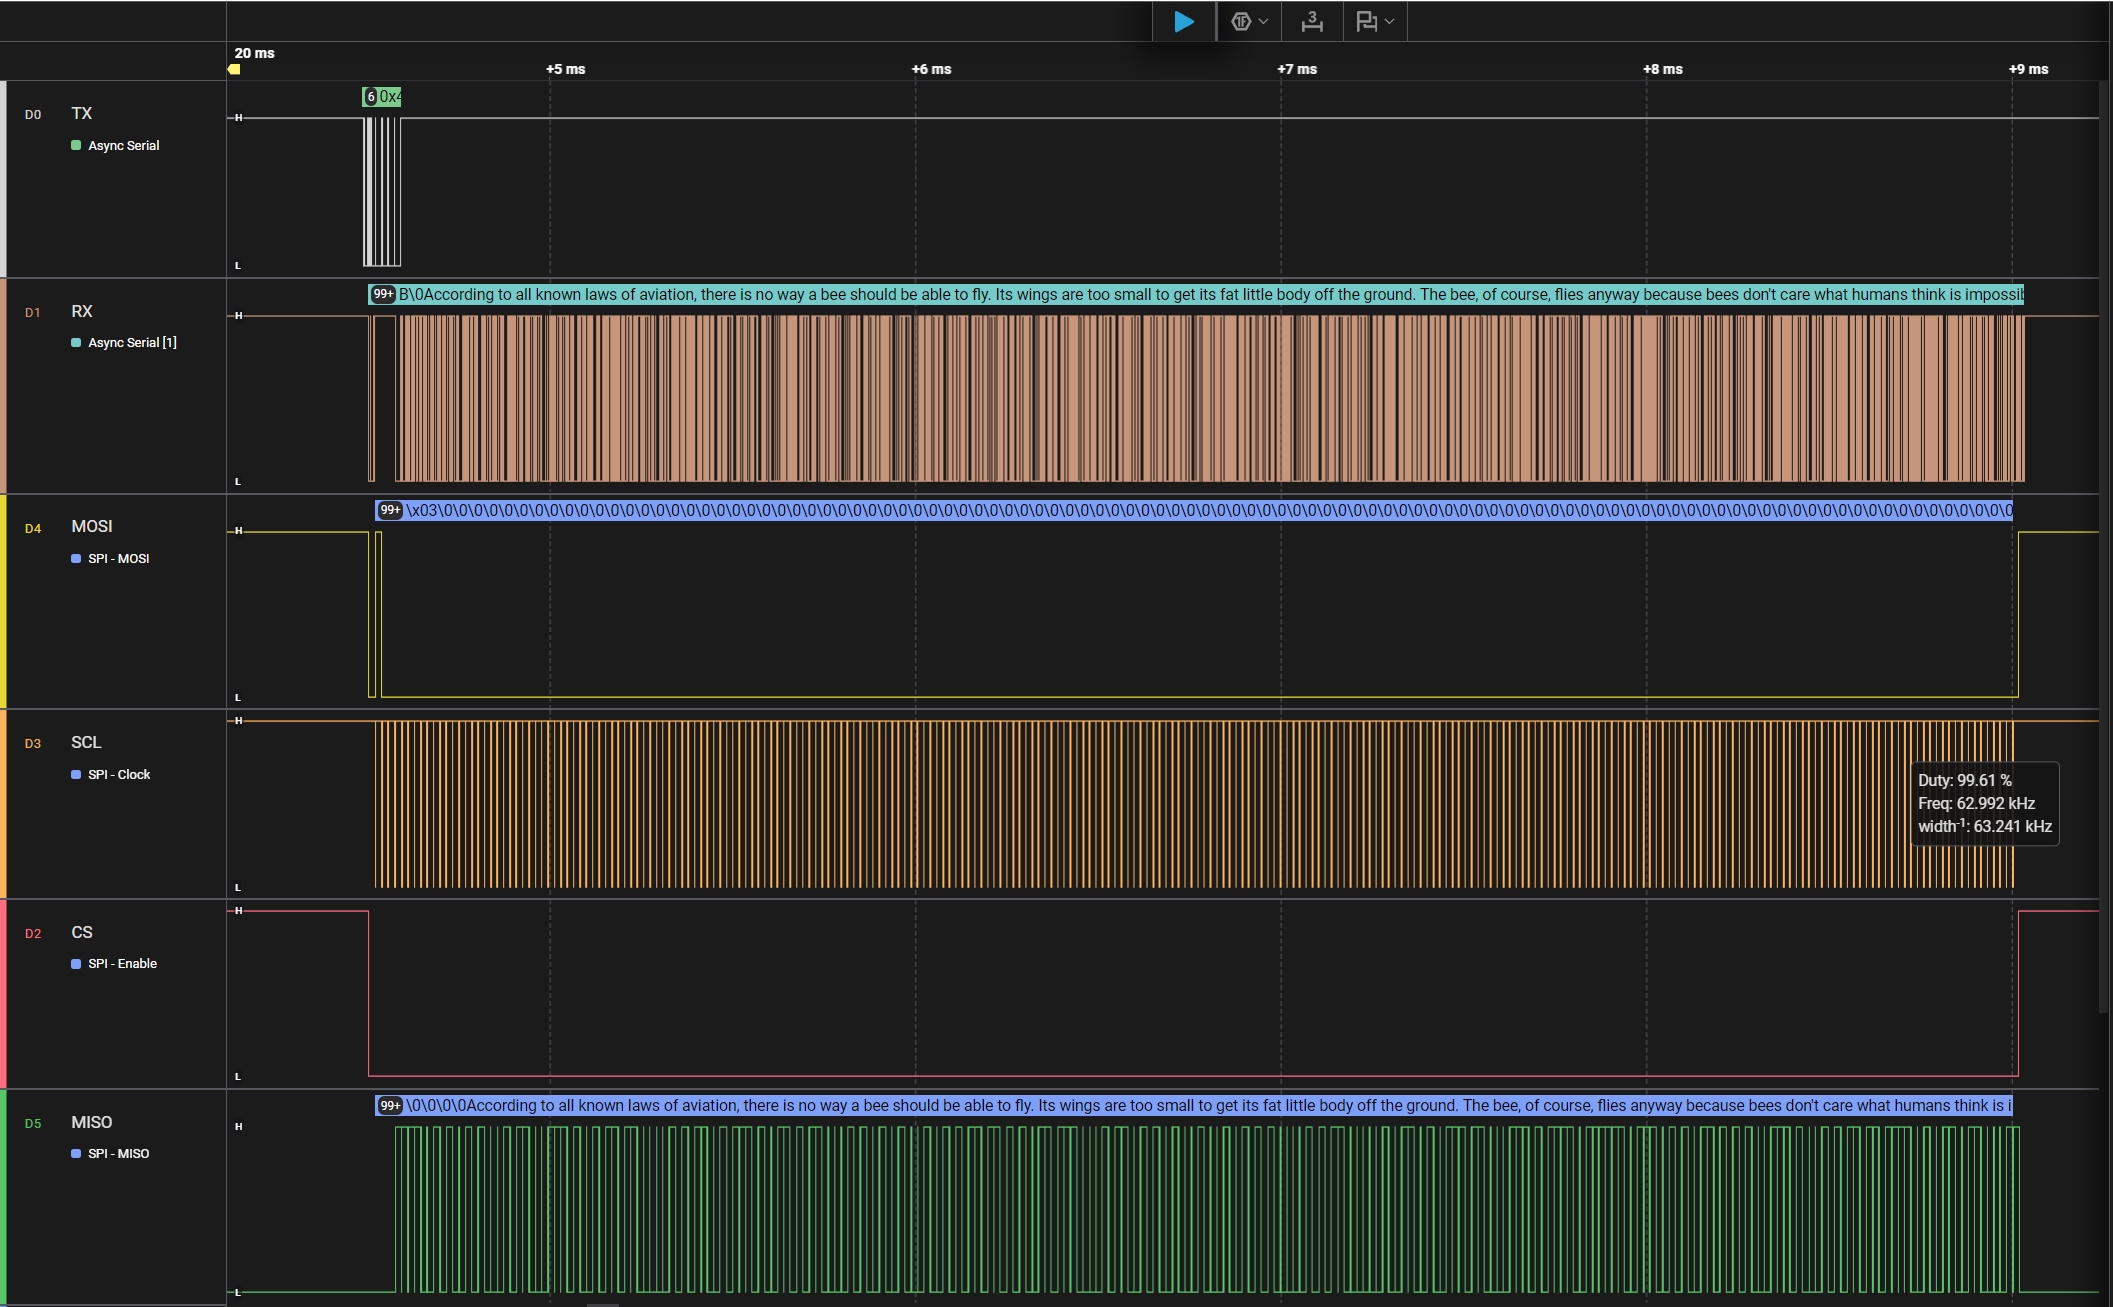
\includegraphics[trim=1mm 1mm 1mm 1mm,scale=0.27]{full spi page package.PNG}
	\caption{SPI read állapot tesztelése}
	\label{SPI read állapot tesztelése}
\end{figure}

A képen látszik, hogy az programozó valóban az összes beírt bájtot helyesen visszaolvassa és elküldi UART-on a PC-nek.

Az SPI read állapot megfelelően működik.

\subsection{I2C write és I2C read állapot tesztelése}
A két állapotot együtt teszteltem, egy utasítás sorral. Az EEPROM-ba egy memória címre beleírtam az Test angol szó ASCII értékét, majd ugyanazt a címet olvastam ki.

A Használt utasítássor az utasítás fájlban:

4400010404000804

46A00000546573740

wait(11ms)

45A00000A10

exit

\begin{itemize}
	\item Az első utasítás azért kell, hogy beállítsuk a I2C kommunikáció hosszát.
	\item A második utasításban a 46 hexadecimális bájt az I2C write állapotot jelöli, az 0000 címre írunk.
	\item A harmadik utasítás egy váró utasítás, ez az EEPROM karakterisztikája miatt szükséges \cite{EEPROM}.
	\item A negyedik utasításban a 45 hexadecimális bájt az I2C read állapotot jelöli, az 0000 címről olvasunk.
\end{itemize}

\subsubsection{A teszt eredménye:}

Log fájl tartalma:

Bytes written: 8

Bytes in queue: 1

Received: 44 

Bytes written: 9

Bytes in queue: 1

Received: 46 

Waiting for 11 ms

Bytes written: 6

Bytes in queue: 5

Received: 45 54 65 73 74 

\subsubsection{Rögzítések:}

\begin{figure}[H]  
	\centering
	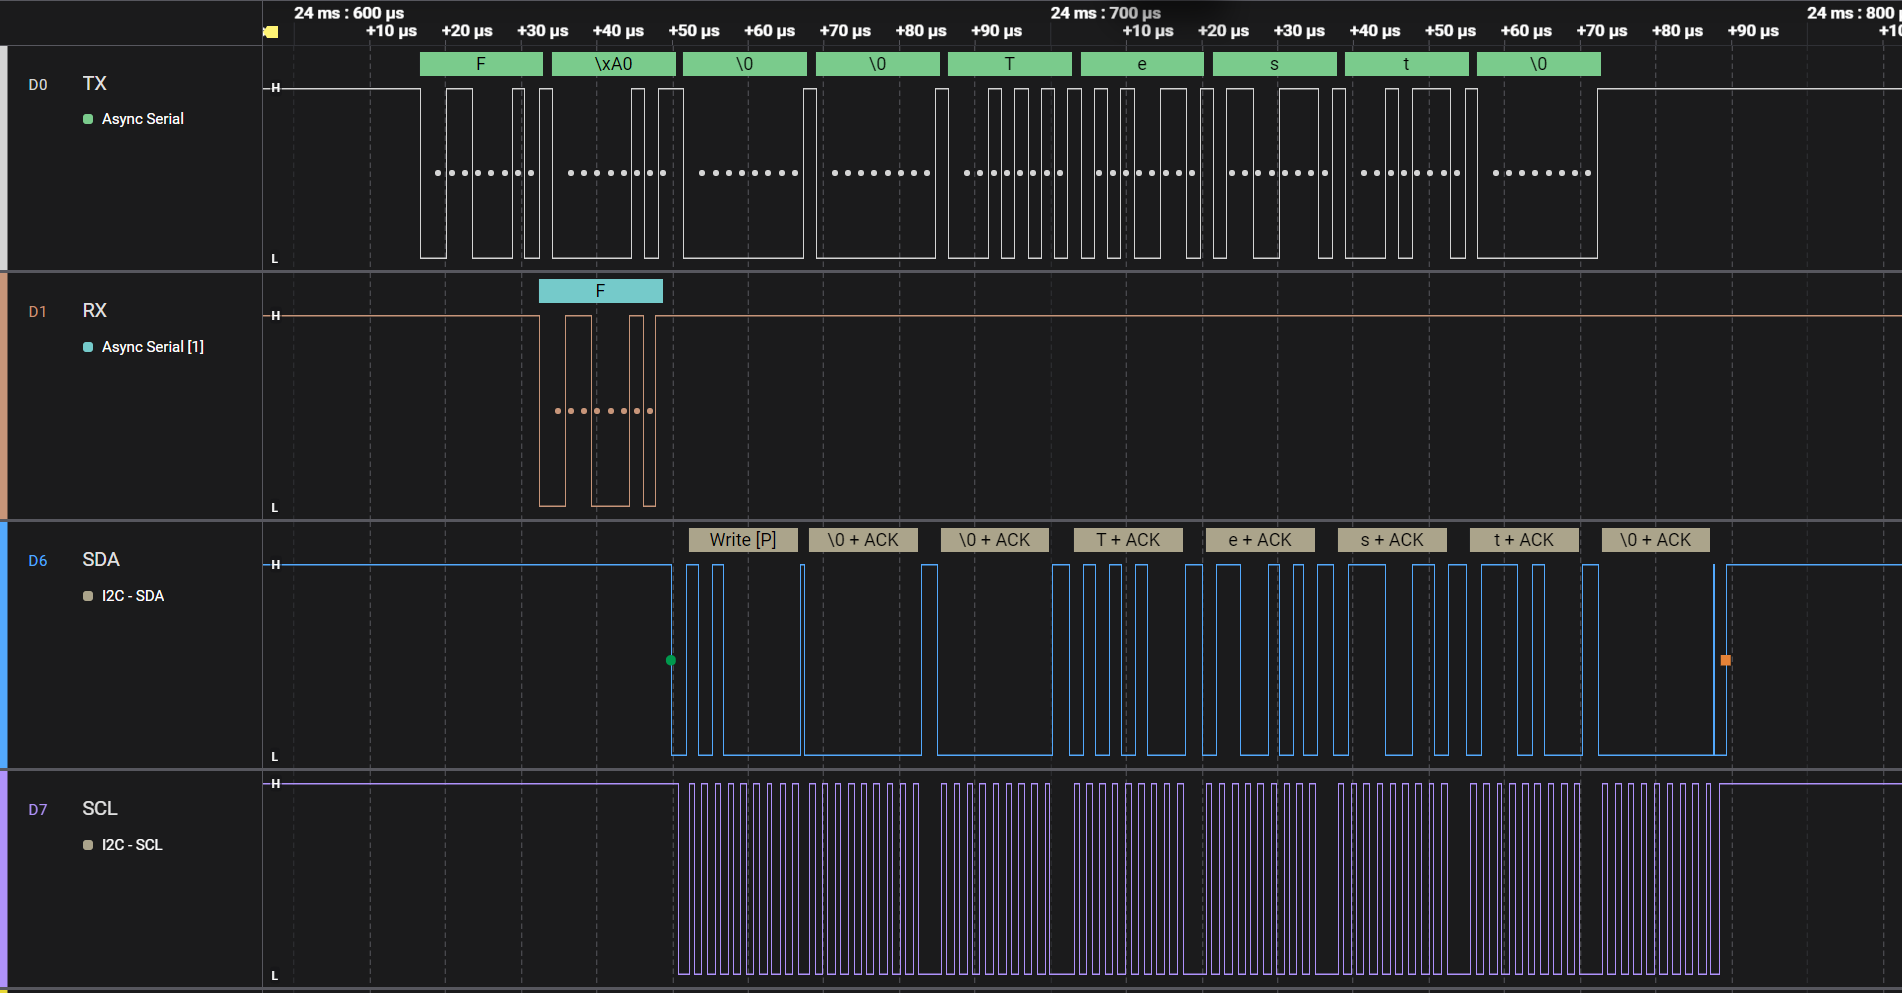
\includegraphics[trim=1mm 1mm 1mm 1mm,scale=0.28]{i2c small write.PNG}
	\caption{I2C write állapot tesztelése}
	\label{I2C write állapot tesztelése}
\end{figure}
Itt látható a helyesen elküldött I2C írás.
\begin{figure}[H]  
	\centering
	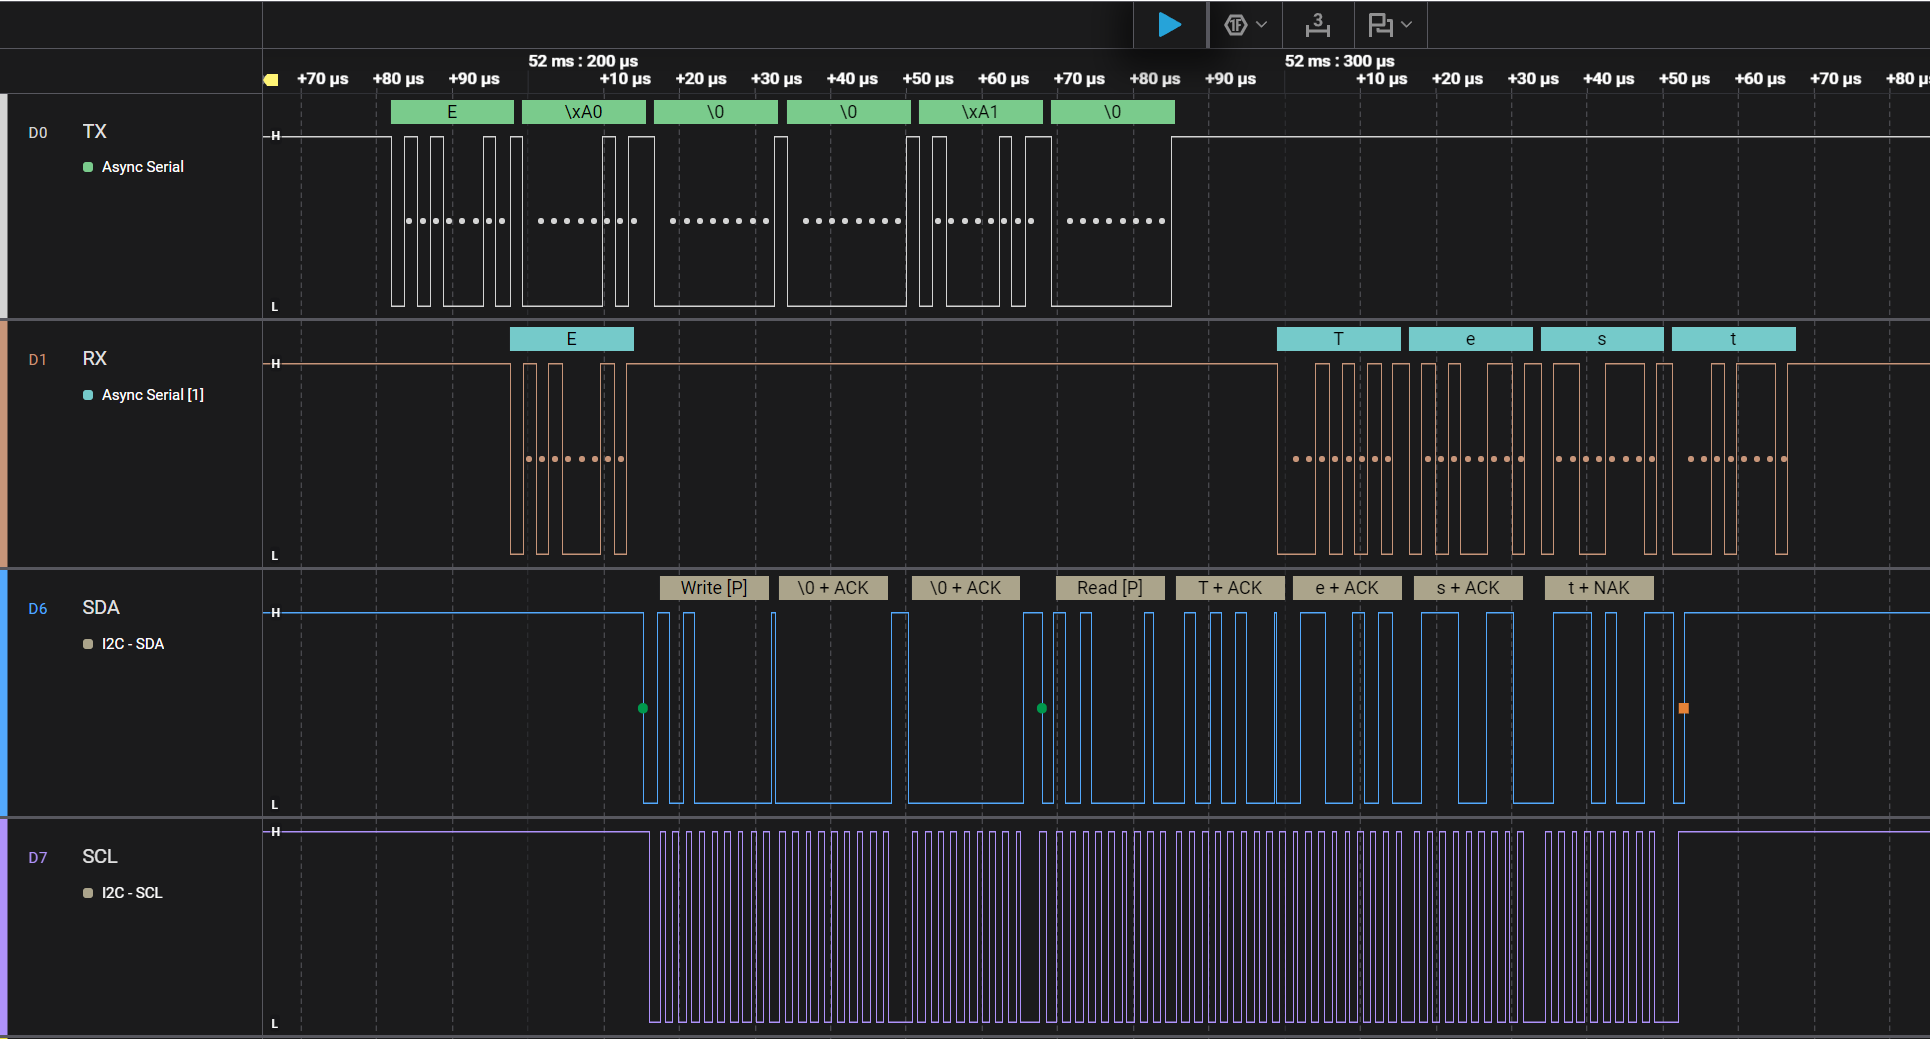
\includegraphics[trim=1mm 1mm 1mm 1mm,scale=0.28]{i2c small read.PNG}
	\caption{I2C read állapot tesztelése}
	\label{I2C read állapot tesztelése}
\end{figure}
Itt pedig a helyes I2C olvasás. A programozó visszaolvasta és visszaküldte az előzőleg  beírt adatokat.

Az I2C read és az I2C write állapot megfelelően működik.

\subsection{Get settings állapot tesztelése}
A diplomamunkámban sok rögzítést mutattam be, ahol látszik, hogy különböző hosszúságú adatkereteket küldött a programozó. A programozót mindig a Get settings állapottal kellett beállítanom. 

Például a \ref{SPI-al kiolvasott gyártó azonosító és típusszám}-as ábra a \pageref{SPI-al kiolvasott gyártó azonosító és típusszám}. oldalon és a \ref{SPI read állapot tesztelése}-as ábra a \pageref{SPI read állapot tesztelése}. oldalon. Itt pedig két külön hosszúságú SPI adatkeret.

A \ref{I2C 1 bájtos olvasás a programozóval}-as. ábra a \pageref{I2C 1 bájtos olvasás a programozóval}. oldalon és a \ref{I2C write állapot tesztelése}-as ábra a \pageref{I2C write állapot tesztelése}. oldalon. Itt pedig két külön hosszúságú I2C adatkeret.

A Get settings állapot megfelelően működik.

\section{Jövőbeli tervek}
Bár az elkészült programozó már most is képes EEPROM és Flash memória egységek programozására SPI és I2C protokollokon keresztül, számos irányba lehetne tovább bővíteni a rendszer funkcionalitását.

Elsőként szeretnék egy grafikus felületet készíteni a jelenlegi C++-ban írt parancssoros vezérlő alkalmazás helyett. Ez felhasználó barátibbá tenné a programozót, és lehetőséget biztosítana a memóriák tartalmának vizuális megjelenítésére, szerkesztésére, valamint jobb fájl alapú kezelése.

Ezen kívül célom újabb protokollok hozzáadása. Ez tovább növelné a programozó eszköz kompatibilitását különféle memóriatípusokkal és más perifériákkal. 

Az protokollok sebesség beállítása most a design része, nem lehet az FPGA konfigurálása után változtatni. Ezt is beállíthatóvá fogom tenni.

Hardveres oldalon, egy a most használt TinyFPGA modul helyett, egy komplexebb FPGA használatával, a rendszer teljesítménye és bővíthetősége is jelentősen növelhető.

Végül, de nem utolsó sorban, szeretnék a projektből egy nyílt forráskódú, dokumentált, mások által is használható eszközt létrehozni. Ez elősegítené, hogy más fejlesztők vagy diákok is tanulhassanak a rendszerből, és akár saját igényeikhez igazítva továbbfejlesszék azt. Az egész forráskód már fent van GitHub-on.

\chapter{Összegzés}

\section{Magyar összefoglaló}
Diplomamunkám célja az volt, hogy egy olyan hardver-szoftver rendszert hozzak létre, amely képes SPI és I2C protokollon keresztül különböző memóriák programozására. A rendszer felépítése egy PC-s vezérlő alkalmazásból, egy UART kommunikáción alapuló interfészből, valamint egy FPGA-ban implementált digitális áramkörből áll. A kommunikációs és vezérlő szoftvert C++ nyelven írtam meg, amely képes parancsokat küldeni, adatokat fogadni és azokat naplózni is.
A VHDL-ben megírt modulokat úgy terveztem, hogy azok rugalmasan konfigurálhatók legyenek, lehetőséggel a kommunikációs keretek hosszának állítására. A tervezett FPGA-s logika tartalmaz SPI és I2C mester egységeket, UART vevő- és adómodulokat, valamint egy fő állapotgépet, amely a beérkező parancsokat feldolgozza. 

A hardveres megvalósítás részeként egy kétrétegű nyákot terveztem a KiCad szoftverrel. A tervezés során igyekeztem törekedni a rugalmasságra, például jumper-ek segítségével különböző feszültségű memóriachipek támogatása is megoldhatóvá vált. 

A rendszer teszteléséhez valós memória modulokat használtam, és logikai analizátor segítségével ellenőriztem a kommunikáció helyességét. 

Összességében a projekt során sikerült elérnem a kitűzött célokat: egy működőképes, használható EEPROM programozót hoztam létre, amely gyakorlati példát szolgáltat az FPGA-k alkalmazására, beágyazott rendszerek fejlesztésében. A munka során jelentős tapasztalatra tettem szert mind a digitális áramkörtervezés, mind az alacsony szintű kommunikációs protokollok kezelése terén.


\section{English summary}
As part of my final year project at the University of Miskolc, I set out to design and implement a configurable EEPROM programmer based on an FPGA platform. My goal was to create a standalone embedded system that would not only deepen my knowledge of FPGA technology and the VHDL hardware description language but also offered practical utility in programming various EEPROM and memory chips via industry-standard communication protocols such as SPI and I2C.

The project integrates both hardware and software development. On the hardware side, I designed a printed circuit board using KiCad, taking into account integrity, power distribution, and flexibility for different memory modules using configurable jumpers. For the FPGA, I wrote the design in VHDL, creating modular components that handle communication, protocol framing, data handling, and control logic. These include UART communication modules for interfacing with a PC, SPI and I2C master modules for memory programming, and internal logic for command parsing and response generation.

On the software side, I developed a command-line interface in C++ for Windows that communicates with the FPGA via a COM port using UART. This interface allows users to send commands, receive responses, and log data from the programmer.
A key challenge in the development was ensuring the precise timing and synchronization of the asynchronous UART and synchronous SPI/I2C protocols. I addressed this through careful selection of clock frequencies and the implementation of robust state machines. Additionally, I conducted extensive testing using logic analyzers and real memory modules to verify the system’s functionality and reliability.

Overall, the project has provided me with valuable experience in embedded system design, digital electronics, and cross-disciplinary engineering skills, bridging software and hardware. I believe the resulting system serves as a useful tool for memory programming tasks and demonstrates the versatile power of FPGA-based solutions.

\chapter{Melléklet}
\begin{itemize}
	\item \href{https://github.com/LordofAllBlue/VHDL-I2C-SPI-Programmer2}{A diplomaunka teljes forráskódja}
\end{itemize}

\renewcommand{\refname}{Irodalomjegyzék}
\begin{thebibliography}{9}
	\bibitem{HDLtestbencs} \href{https://nandland.com/what-is-a-testbench/}{Nandland: what is a testbench}

	\bibitem{vhdl} \href{https://nandland.com/what-is-a-testbench/}{Dr. Steve Arar: What Is VHDL? Getting Started with Hardware Description Language for Digital Circuit Design}

	\bibitem{fpga} \href{https://moodle.tktk.ee/pluginfile.php/270005/mod_resource/content/1/Harris%20D.%20M.%2C%20Harris%20S.%20L.%20-%20Digital%20Design%20and%20Computer%20Architecture%2C%202nd%20Edition%20-%202012.pdf}{S. Trimberger, Field-Programmable Gate Array Technology, Springer, 1994.}


	\bibitem{tiuart} \href{https://www.ti.com/lit/an/sbaa565/sbaa565.pdf?ts=1747843344270&ref_url=https%253A%252F%252Fwww.google.com%252F}{Texas Instruments: KeyStone Architecture Universal Asynchronous Receiver/Transmitter (UART)}

	\bibitem{ti3c} \href{https://www.ti.com/lit/an/sbaa565/sbaa565.pdf?ts=1747843344270&ref_url=https%253A%252F%252Fwww.google.com%252F}{Texas Instruments: A Basic Guide to I2C}

	\bibitem{tispi} \href{https://www.ti.com/lit/ug/sprugp2a/sprugp2a.pdf?ts=1747856353194&ref_url=https%253A%252F%252Fwww.google.com%252F}{Texas Instruments: KeyStone Architecture Serial Peripheral Interface (SPI)}

    \bibitem{fpgaadatlap} \href{https://datasheet.octopart.com/LCMXO2-4000HC-4MG132I-Lattice-Semiconductor-datasheet-12584740.pdf}{A MachXO2 FPGA család adatlapja }
	 \bibitem{EEPROM} \href{https://ww1.microchip.com/downloads/en/DeviceDoc/doc0670.pdf}{A AT24C256 EEPROM adatlapja }
	\bibitem{FLASH} \href{https://ww1.microchip.com/downloads/en/DeviceDoc/doc0670.pdf}{A W25Q64FV FLASH adatlapja }
\end{thebibliography}





\end{document}